\section{Determining stable spinodal compositions}
The Hessian of the demixing free energy is used to identify stable spinodal compositions. By analyzing the values of $\Delta F$, the range of chromium compositions where spinodal demixing is stable could be determined. This information is crucial for understanding the behavior of materials undergoing demixing processes and provides insights into their stability. Verifying phase transition indicators enable investigating properties to detect these phase transitions. 

Thermodynamics of demixing for body-centered cubic iron-chrome alloy calculated as a function of chromium composition. \cite{korzhavyi2009electronic,trochet2021influence,levesque2011simple, binder2001spinodal}(a) Enthalpy of demixing. (b) Entropy of demixing. (c) Free energy of demixing. 



\section{Obtaining elastic tensor from quantum mechanical calculations}
Quantum mechanical calculations provide a means to obtain the elastic tensor, a key parameter for characterizing material behavior. By employing thermoelastic equations derived from statistical mechanics, the elastic tensor could be determined from self-consistent field calculations for atomic positions from the electron density to gain insights into the elastodynamic properties of materials with lattice dynamic theory and other theoretical frameworks.

Elastic tensor from density functional theory calculations for body-centered cubic iron-chrome alloys as a function of chromium content. Stiffening is evident from increasing elastic constants with increasing chromium. \cite{korzhavyi2009electronic,razumovskiy2011first}

\subsection{Calculating elastic moduli and assessing embrittlement criteria}
Elastic moduli from quantum mechanical elastic tensor for body-centered cubic iron-chrome alloys as a function of chromium content. Stiffening is evident from increasing elastic moduli with increasing chromium. \cite{korzhavyi2009electronic,razumovskiy2011first}




\section{Predicting plastic embrittlement through quantum elastodynamics}
Quantum elastodynamics offers a means to predict plastic embrittlement in materials.  We could explore the relationship between stiffening and embrittlement using the elastic moduli obtained from quantum elastodynamics. 


\begin{figure}[!ht]
	\centering
	\begin{subfigure}{0.9\textwidth}
         \centering
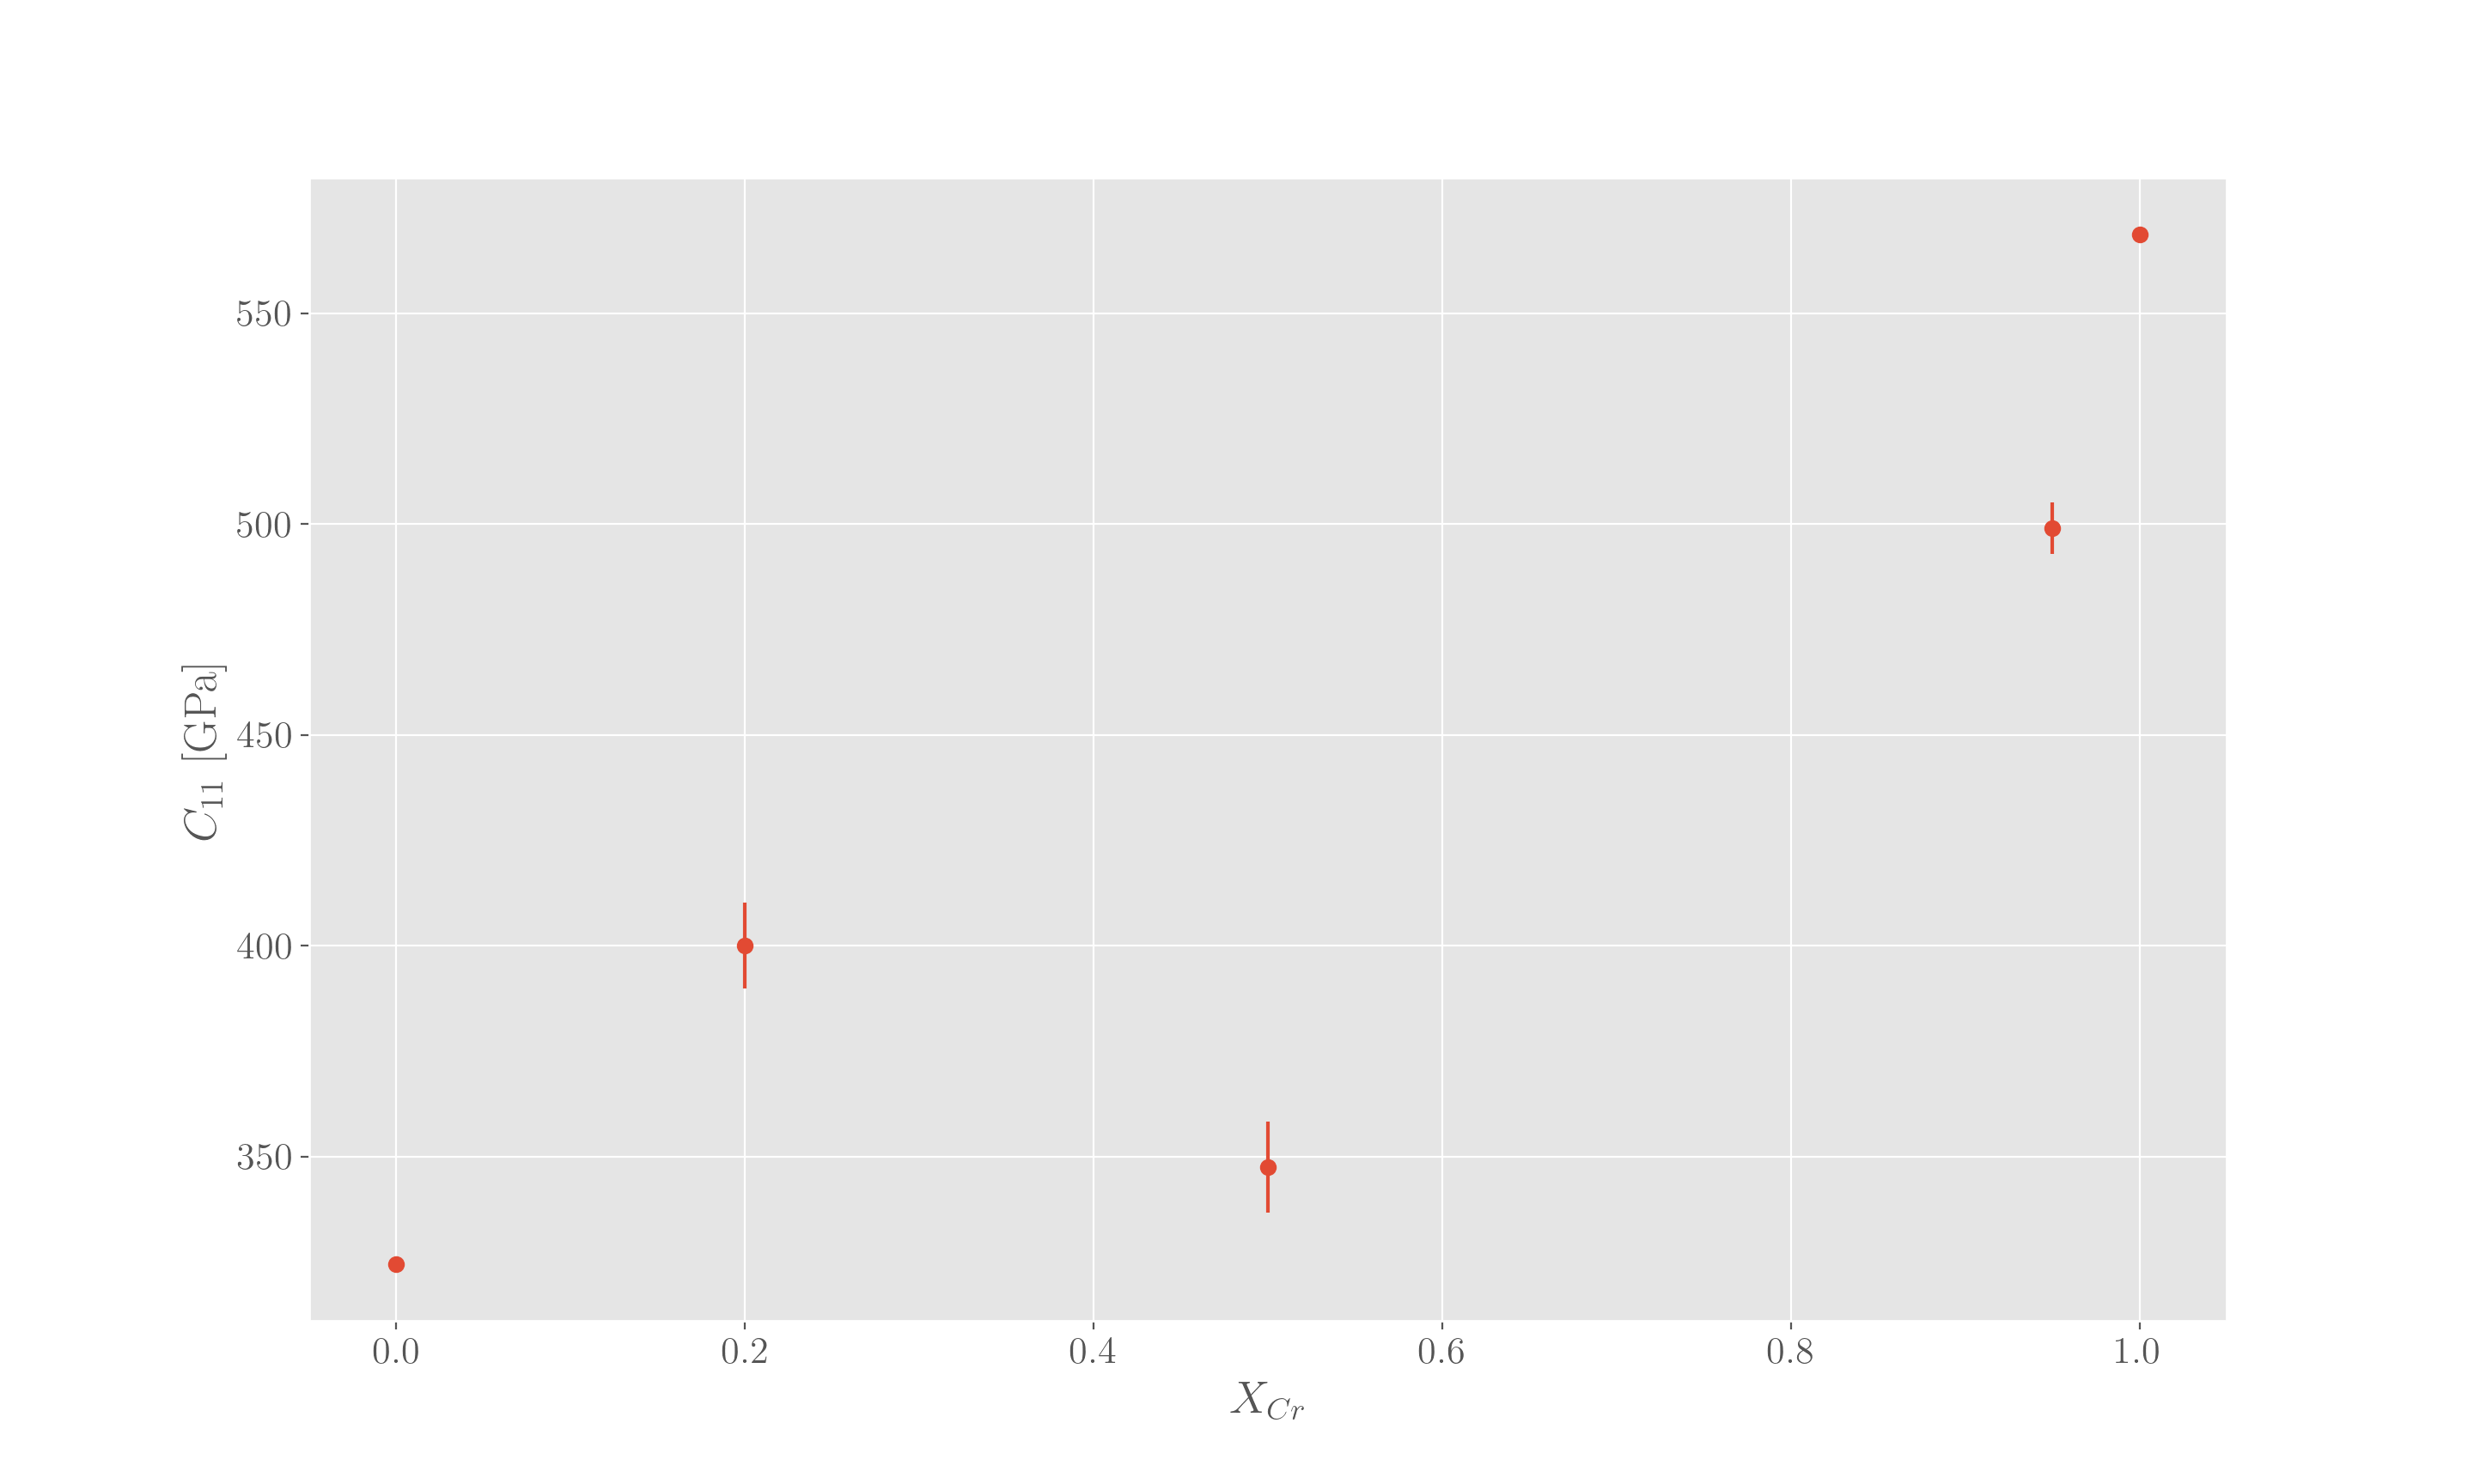
\includegraphics[width=\linewidth, left]{Parts/Figures/C11.png}
         \caption{Normal constant, $C_{11}$}
         \label{fig1a}
     \end{subfigure}
     \hfill
     \begin{subfigure}{0.45\textwidth}
         \centering
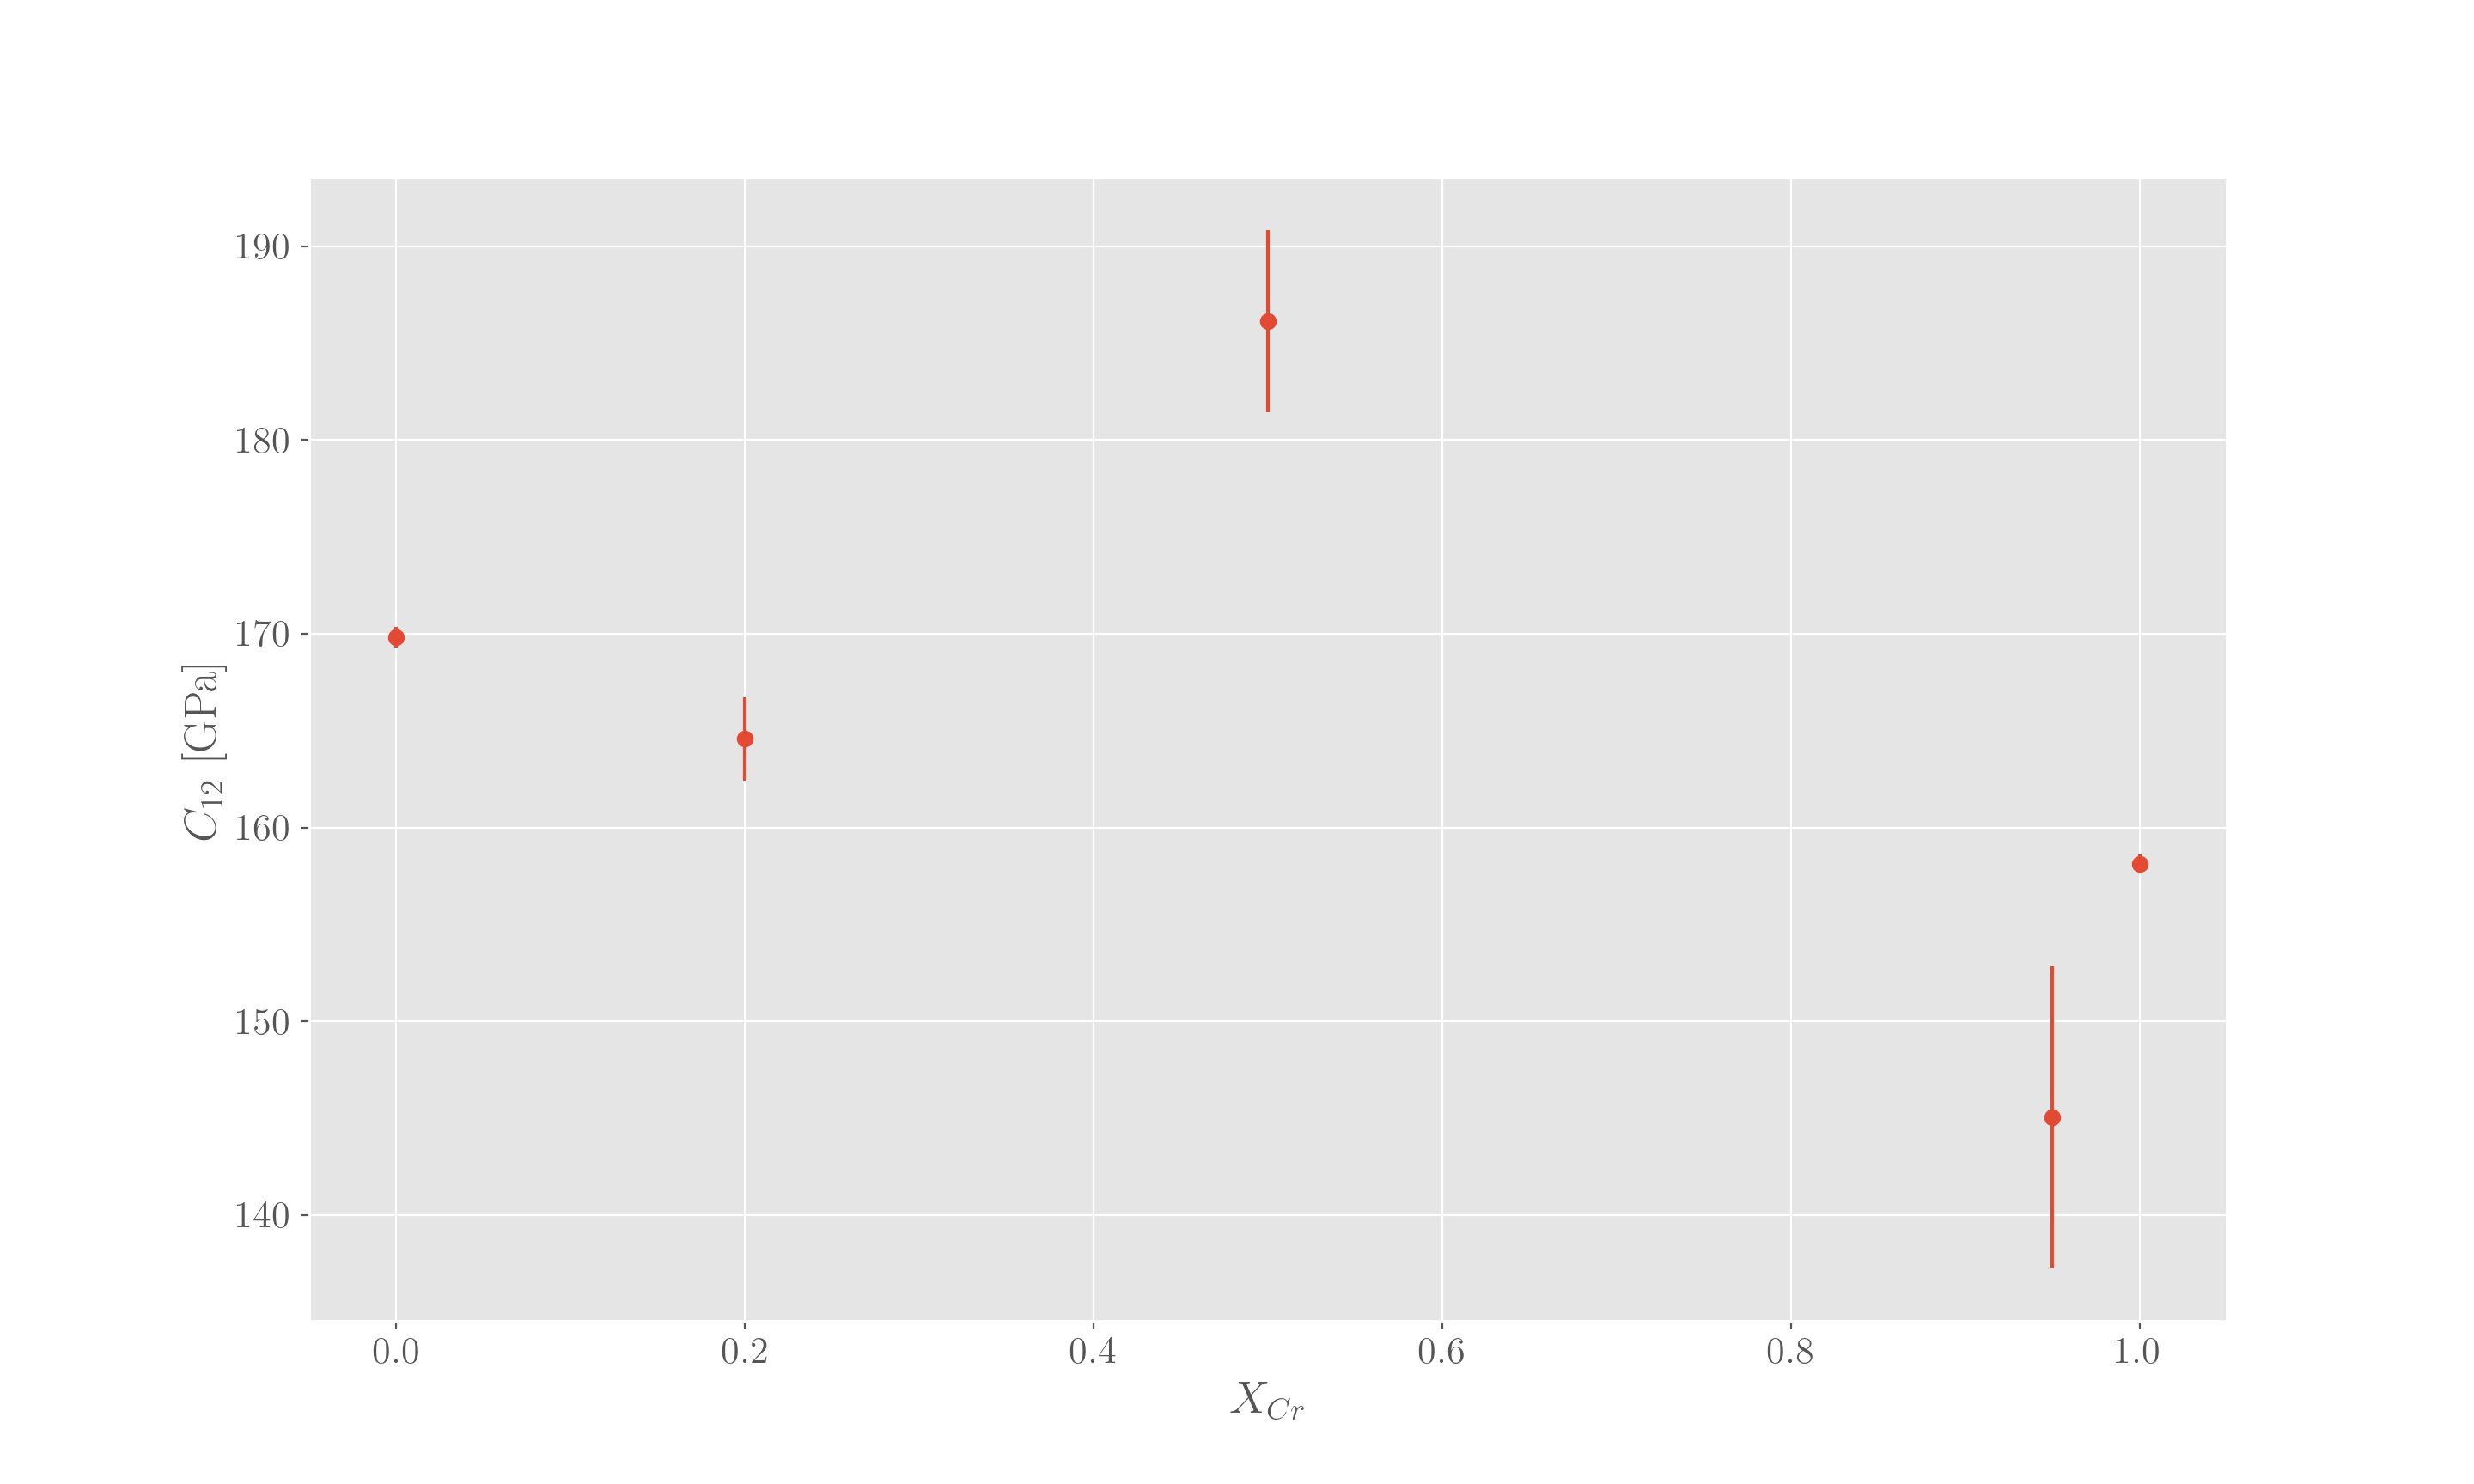
\includegraphics[width=\linewidth, right]{Parts/Figures/C12.png}         \caption{$C_{12}$}
         \label{fig1b}
         \end{subfigure}
          \hfill
     \begin{subfigure}{0.45\textwidth}
         \centering
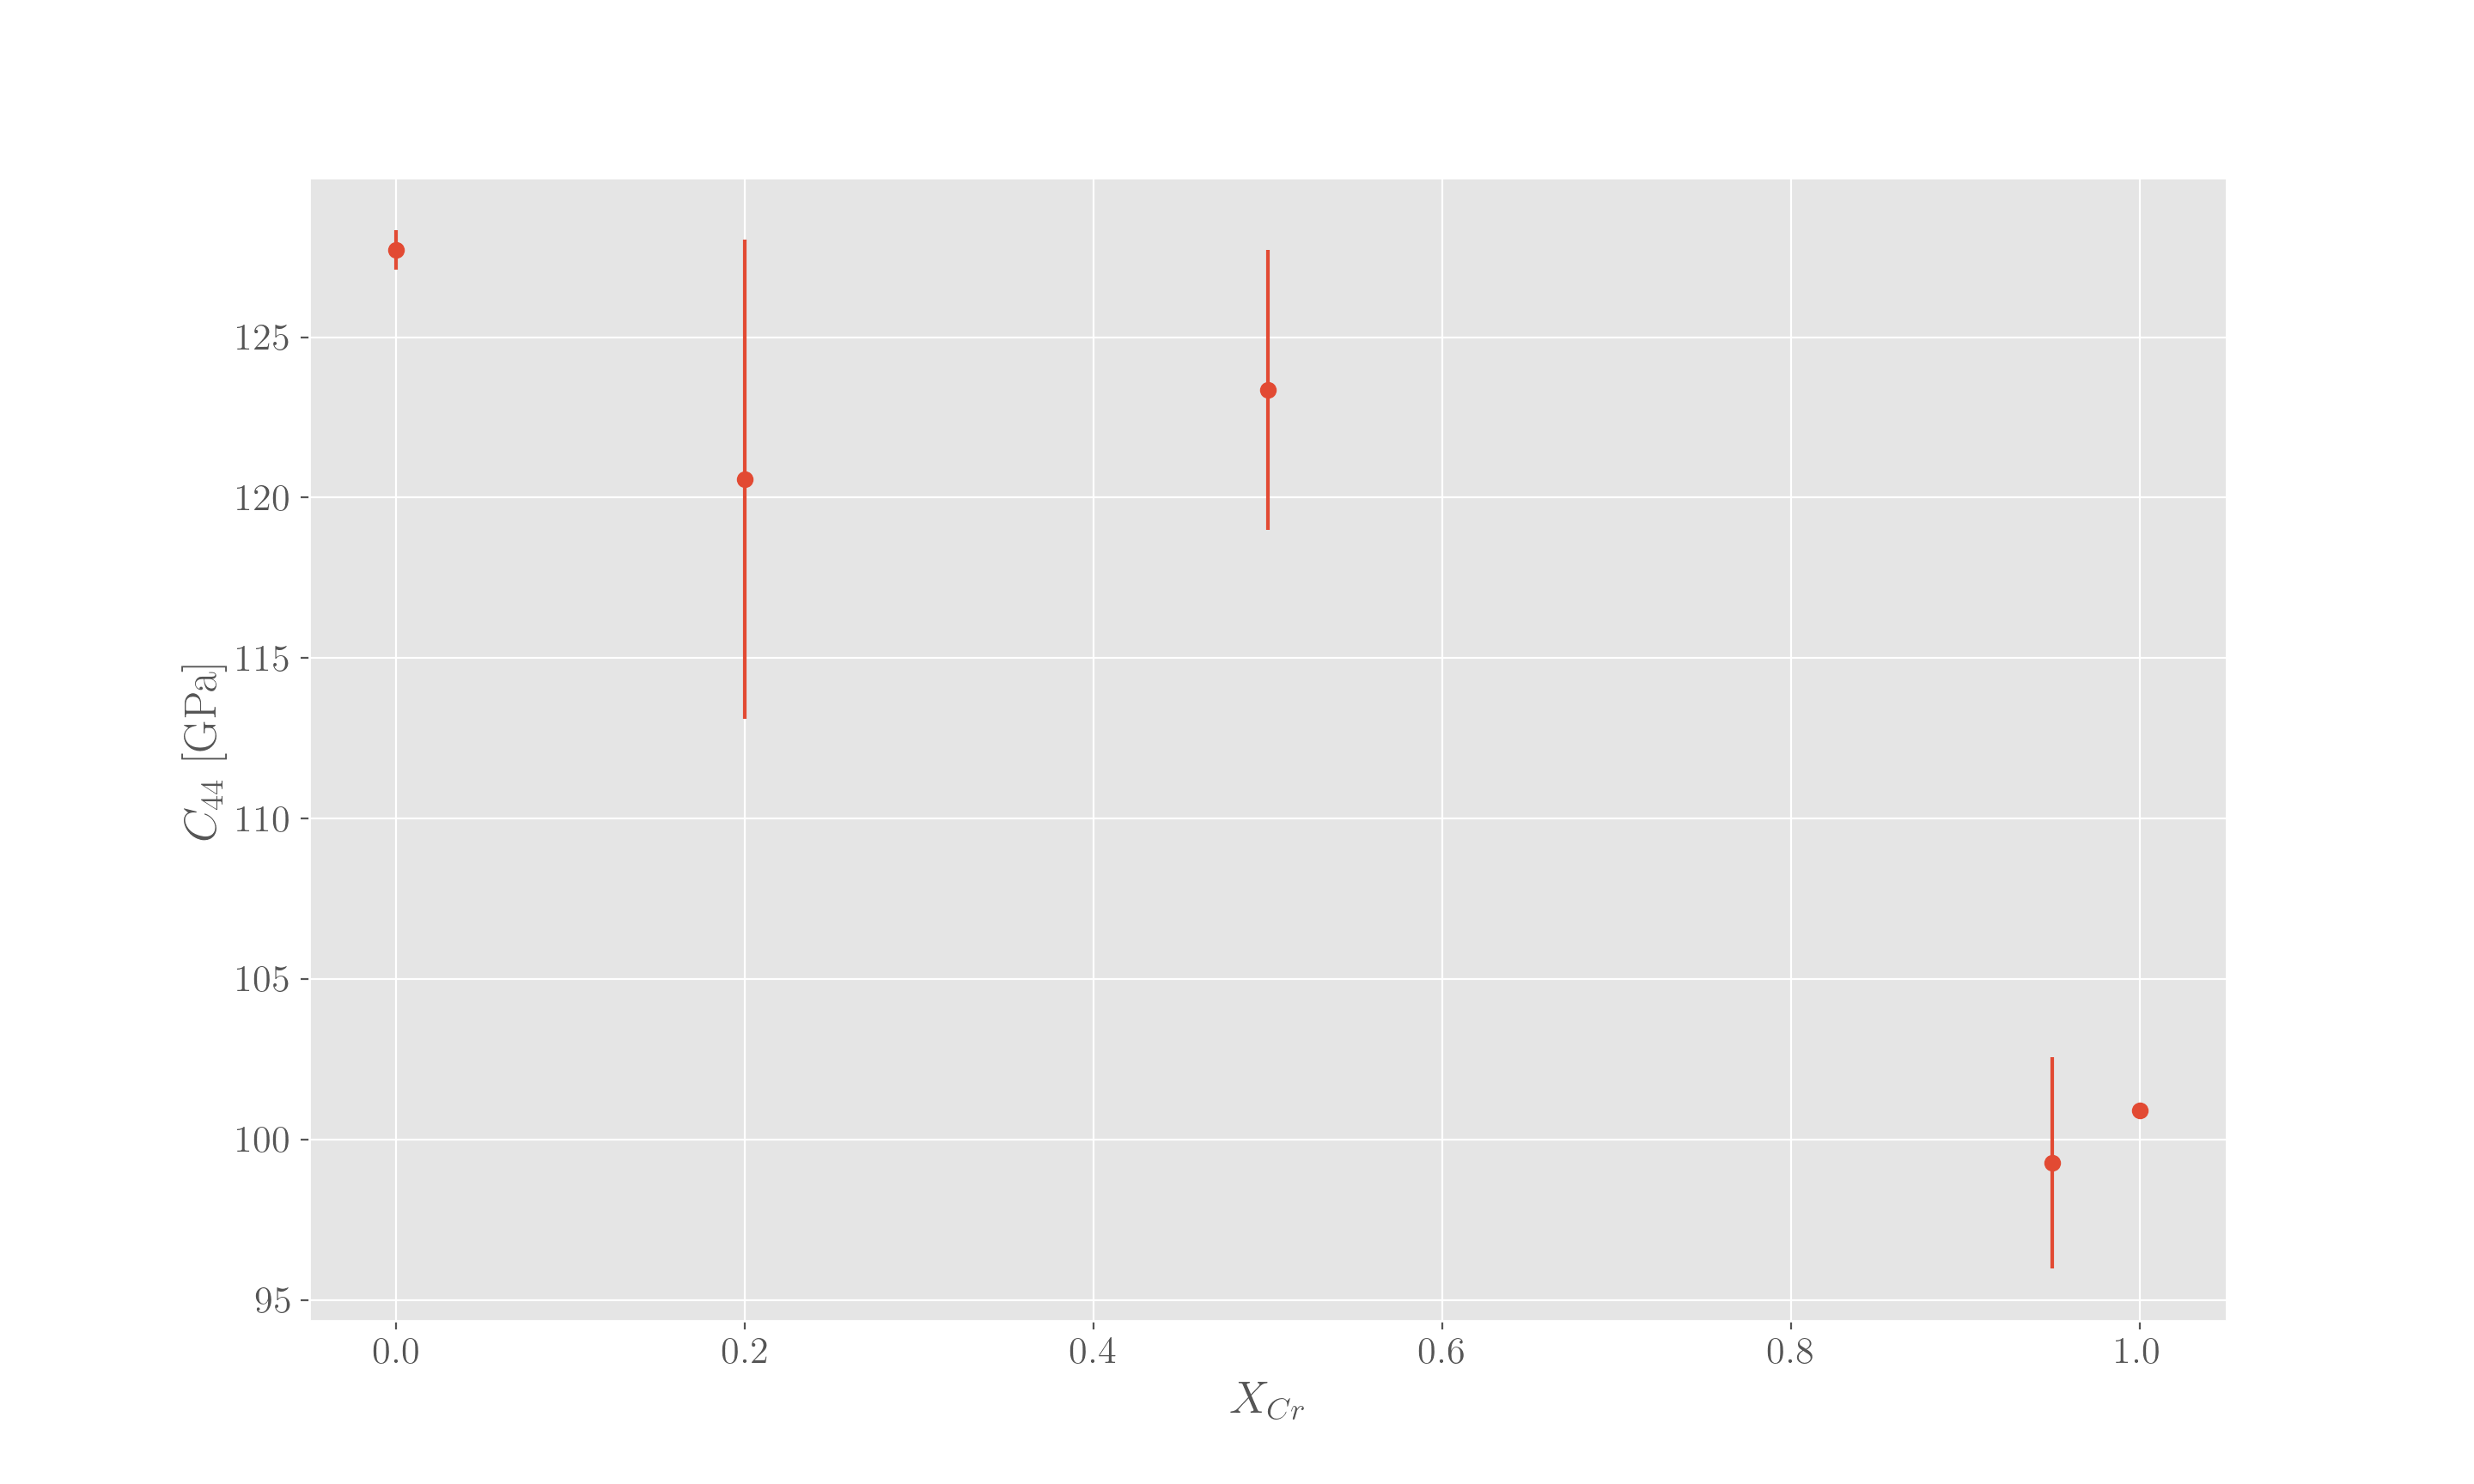
\includegraphics[width=\linewidth, right]{Parts/Figures/C44.png}         \caption{Shear constant, $C_{44}$}
         \label{fig1c}
     \end{subfigure}
	\caption{Elastic constants of bcc binary FeCr as a function of Cr composition indicate spinodal decomposition-induced stiffening towards embrittlement. The trends and values are consistent with theoretical and experimental results reported in literature. [REF] (a) ... (b) ... (c) ...}
	\label{fig1}
\end{figure}



\begin{comment}
    

\begin{figure}[!ht]
	\centering
	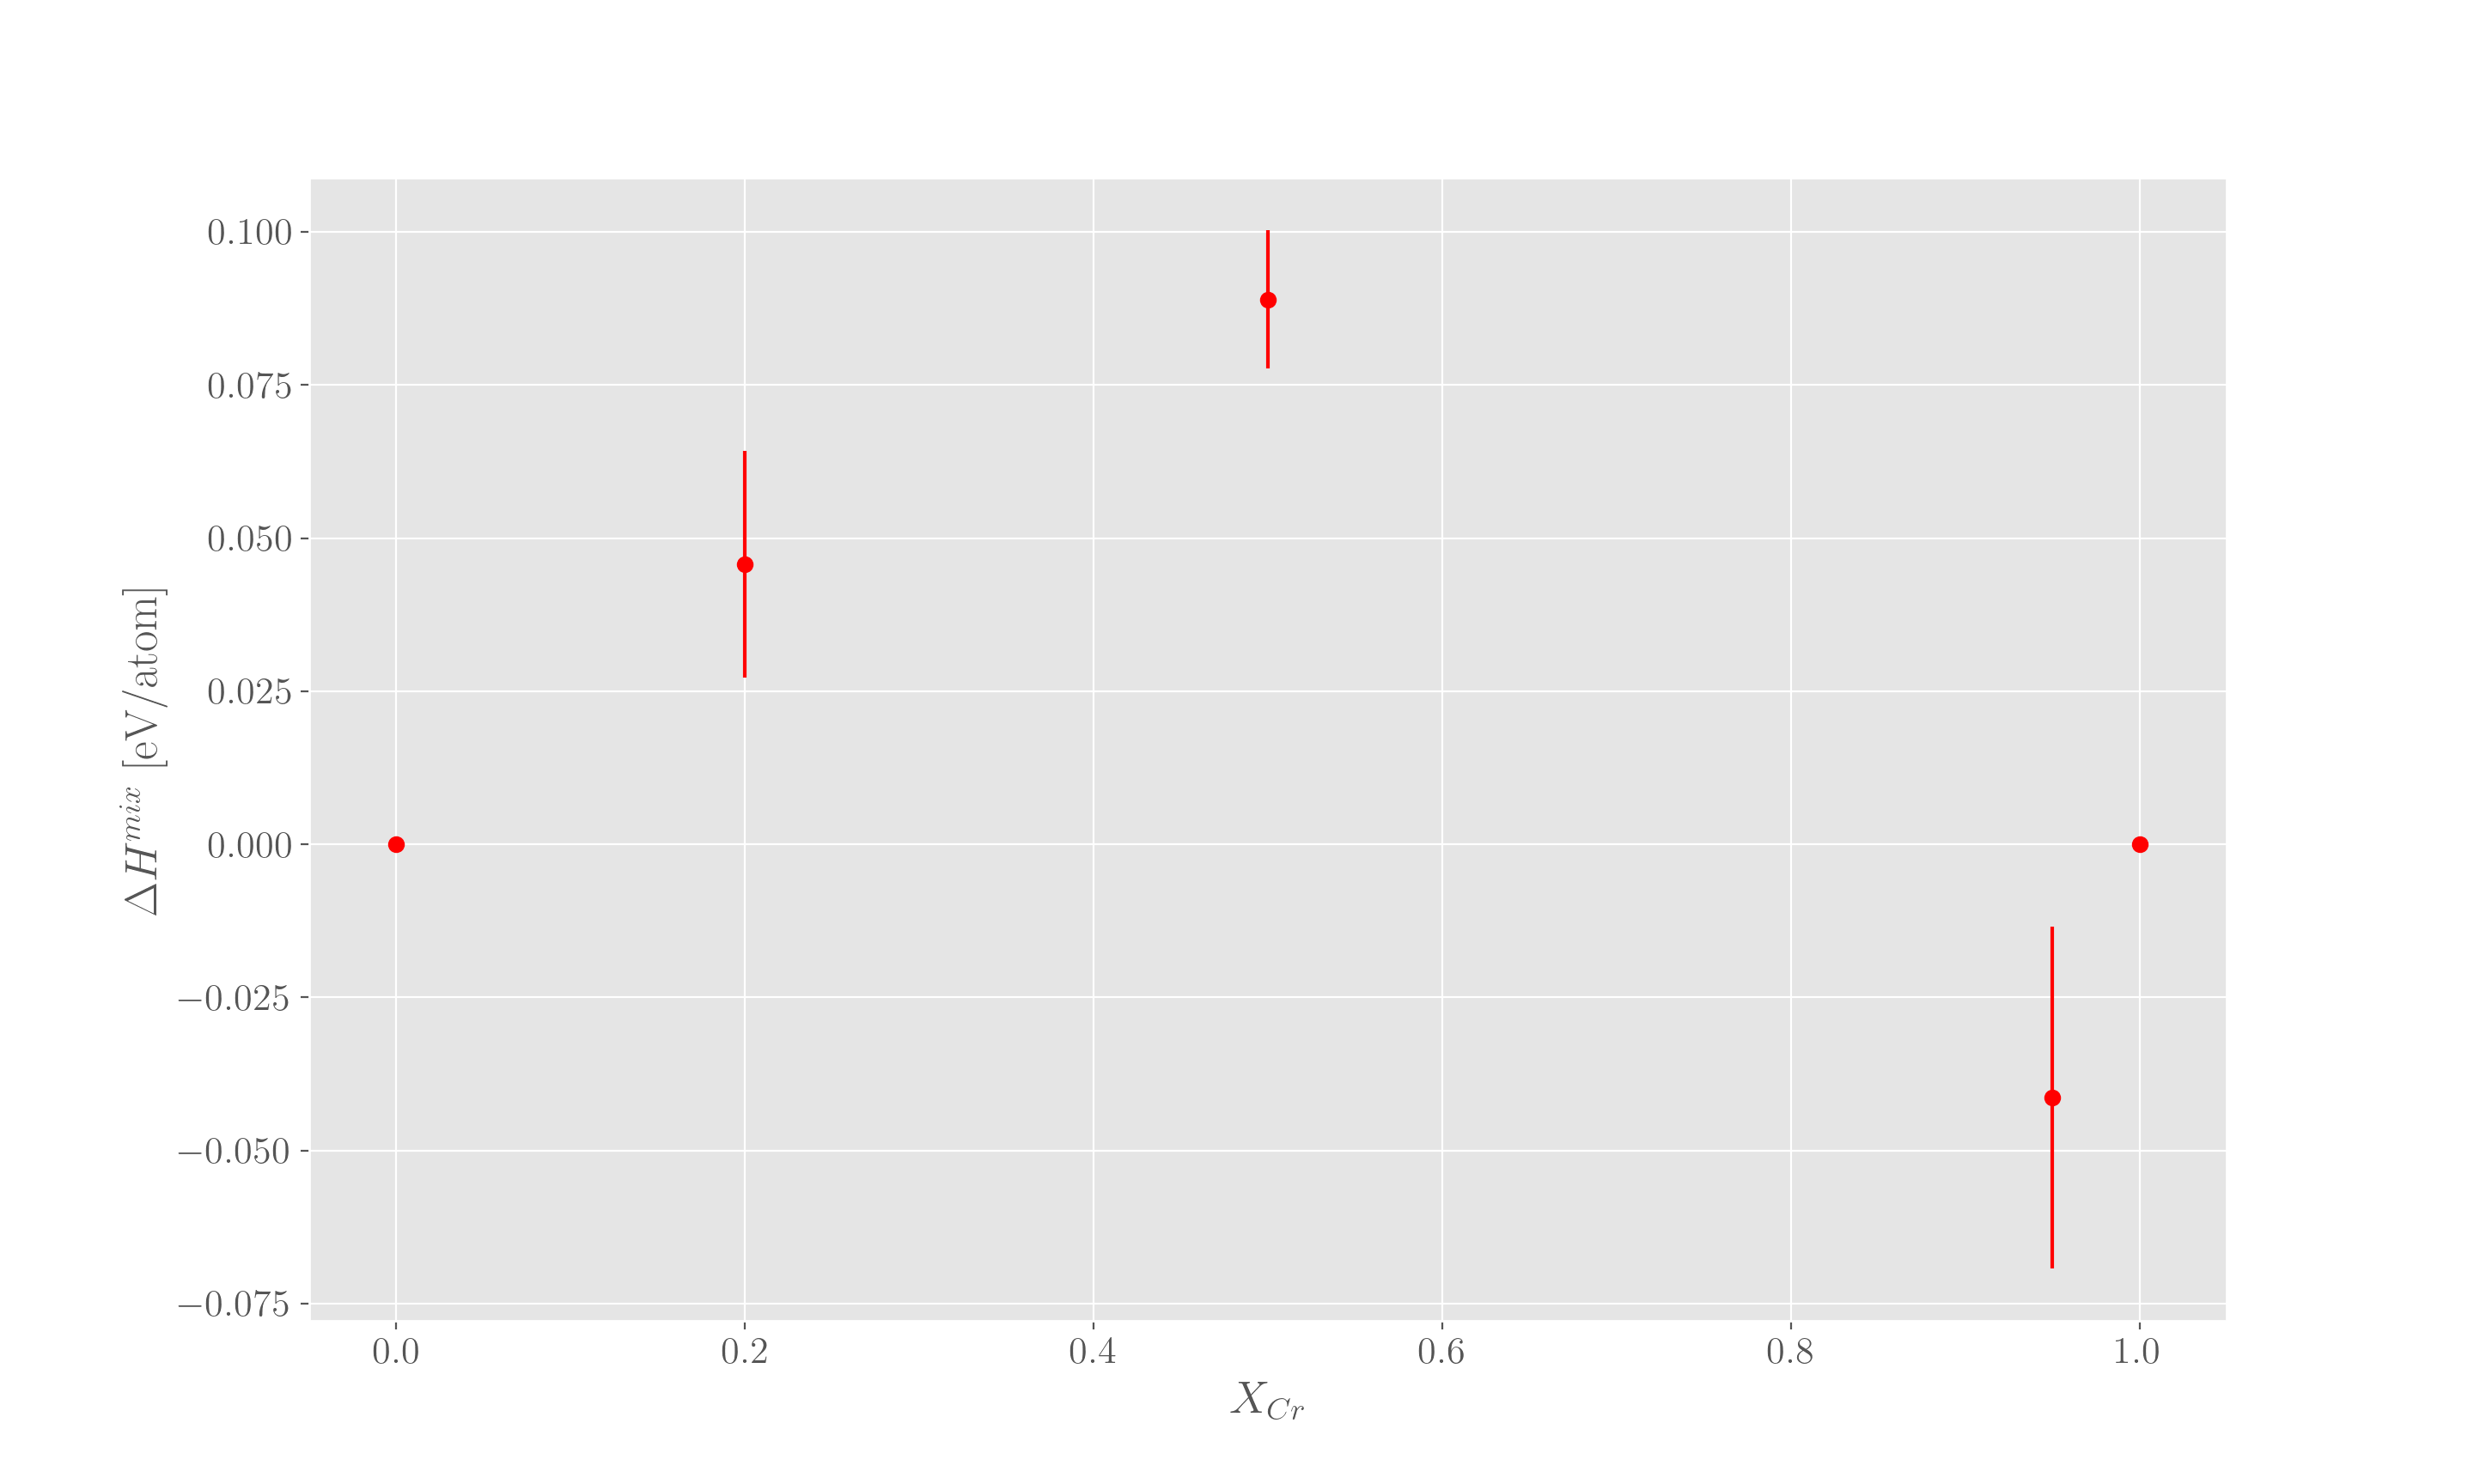
\includegraphics[width=0.9\textwidth]{Parts/Figures/Hmix-vF.png}
	\caption{Negative mixing enthalpy of Fe and Cr in a binary alloy indicate unmixing in the form of spinodal decomposition is thermodynamically favorable in bcc $\delta$-ferrite in cast austenitic stainless steels. The mixing enthalpy is calculated as difference between the \emph{ab initio} relaxation enthalpy of the binary alloy and the pure elements and verifies that the simulated alloys are under spinodal decomposition conditions. }
	\label{fig1}
\end{figure}
\end{comment}

\begin{comment}
    
\begin{figure}[!ht]
	\centering
	\begin{subfigure}{0.9\textwidth}
         \centering
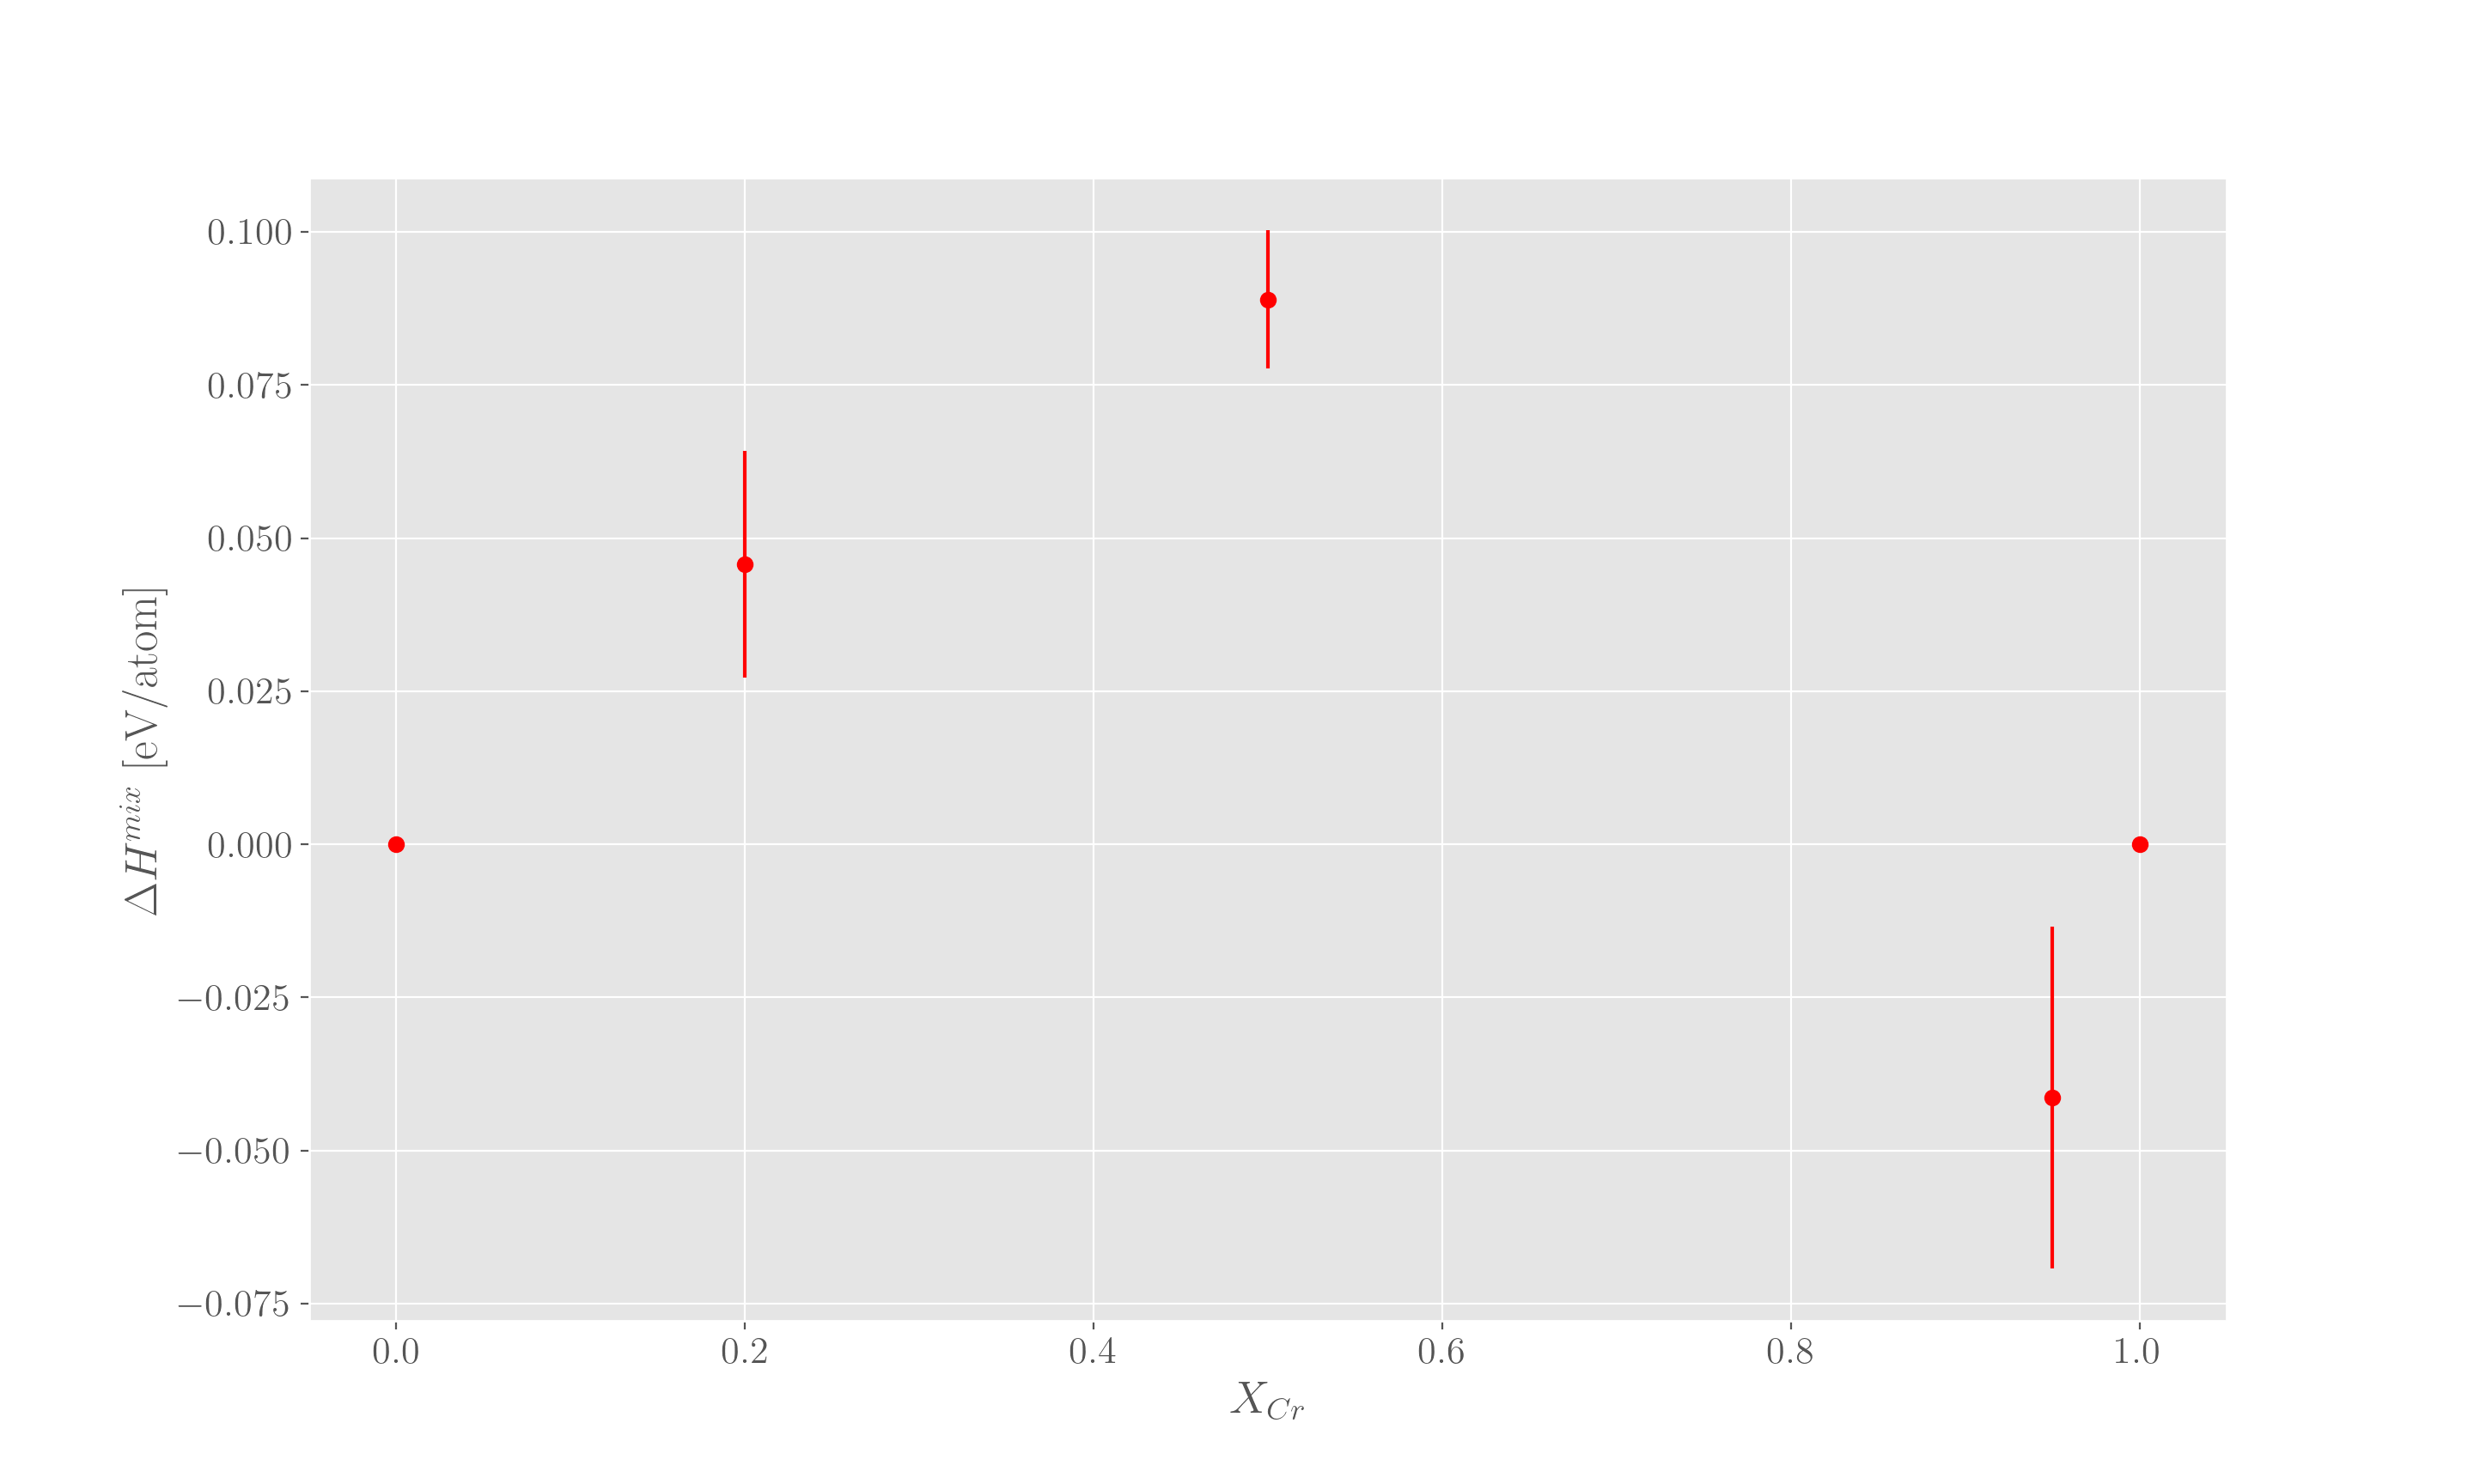
\includegraphics[width=\linewidth, left]{Parts/Figures/Hmix-vF.png}
         \caption{Enthalpy of mixing}
         \label{fig1a}
     \end{subfigure}
     \hfill
     \begin{subfigure}{0.45\textwidth}
         \centering
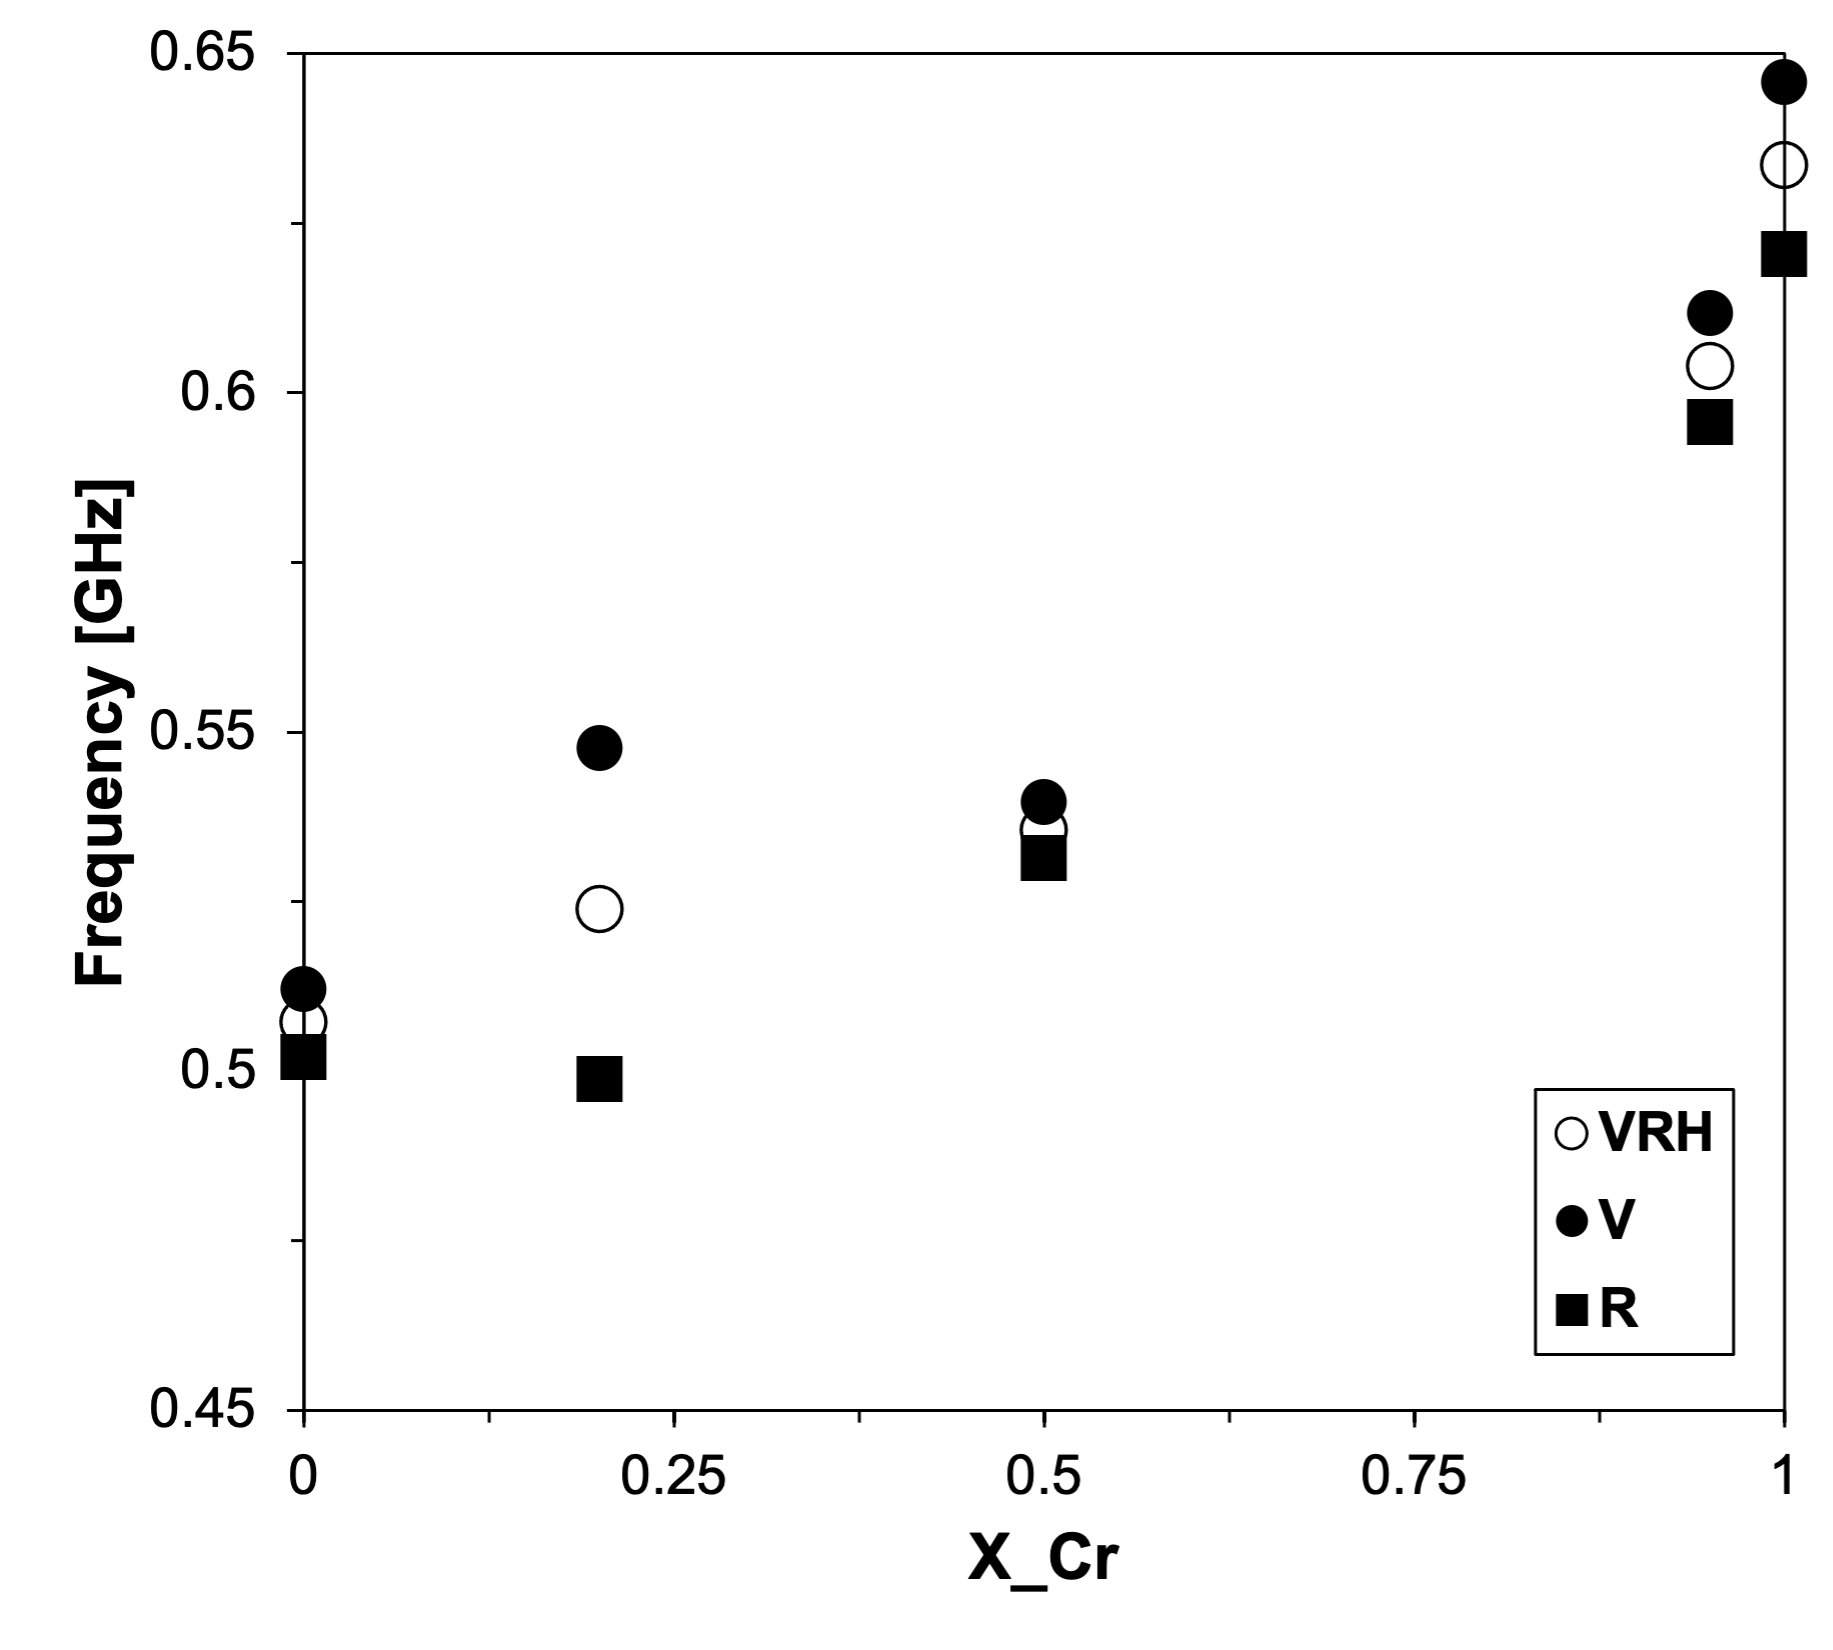
\includegraphics[width=\linewidth, right]{Parts/Figures/rayleigh-wave-3.png}         \caption{Rayleigh wave frequencies}
         \label{fig1b}
         \end{subfigure}
          \hfill
     \begin{subfigure}{0.45\textwidth}
         \centering
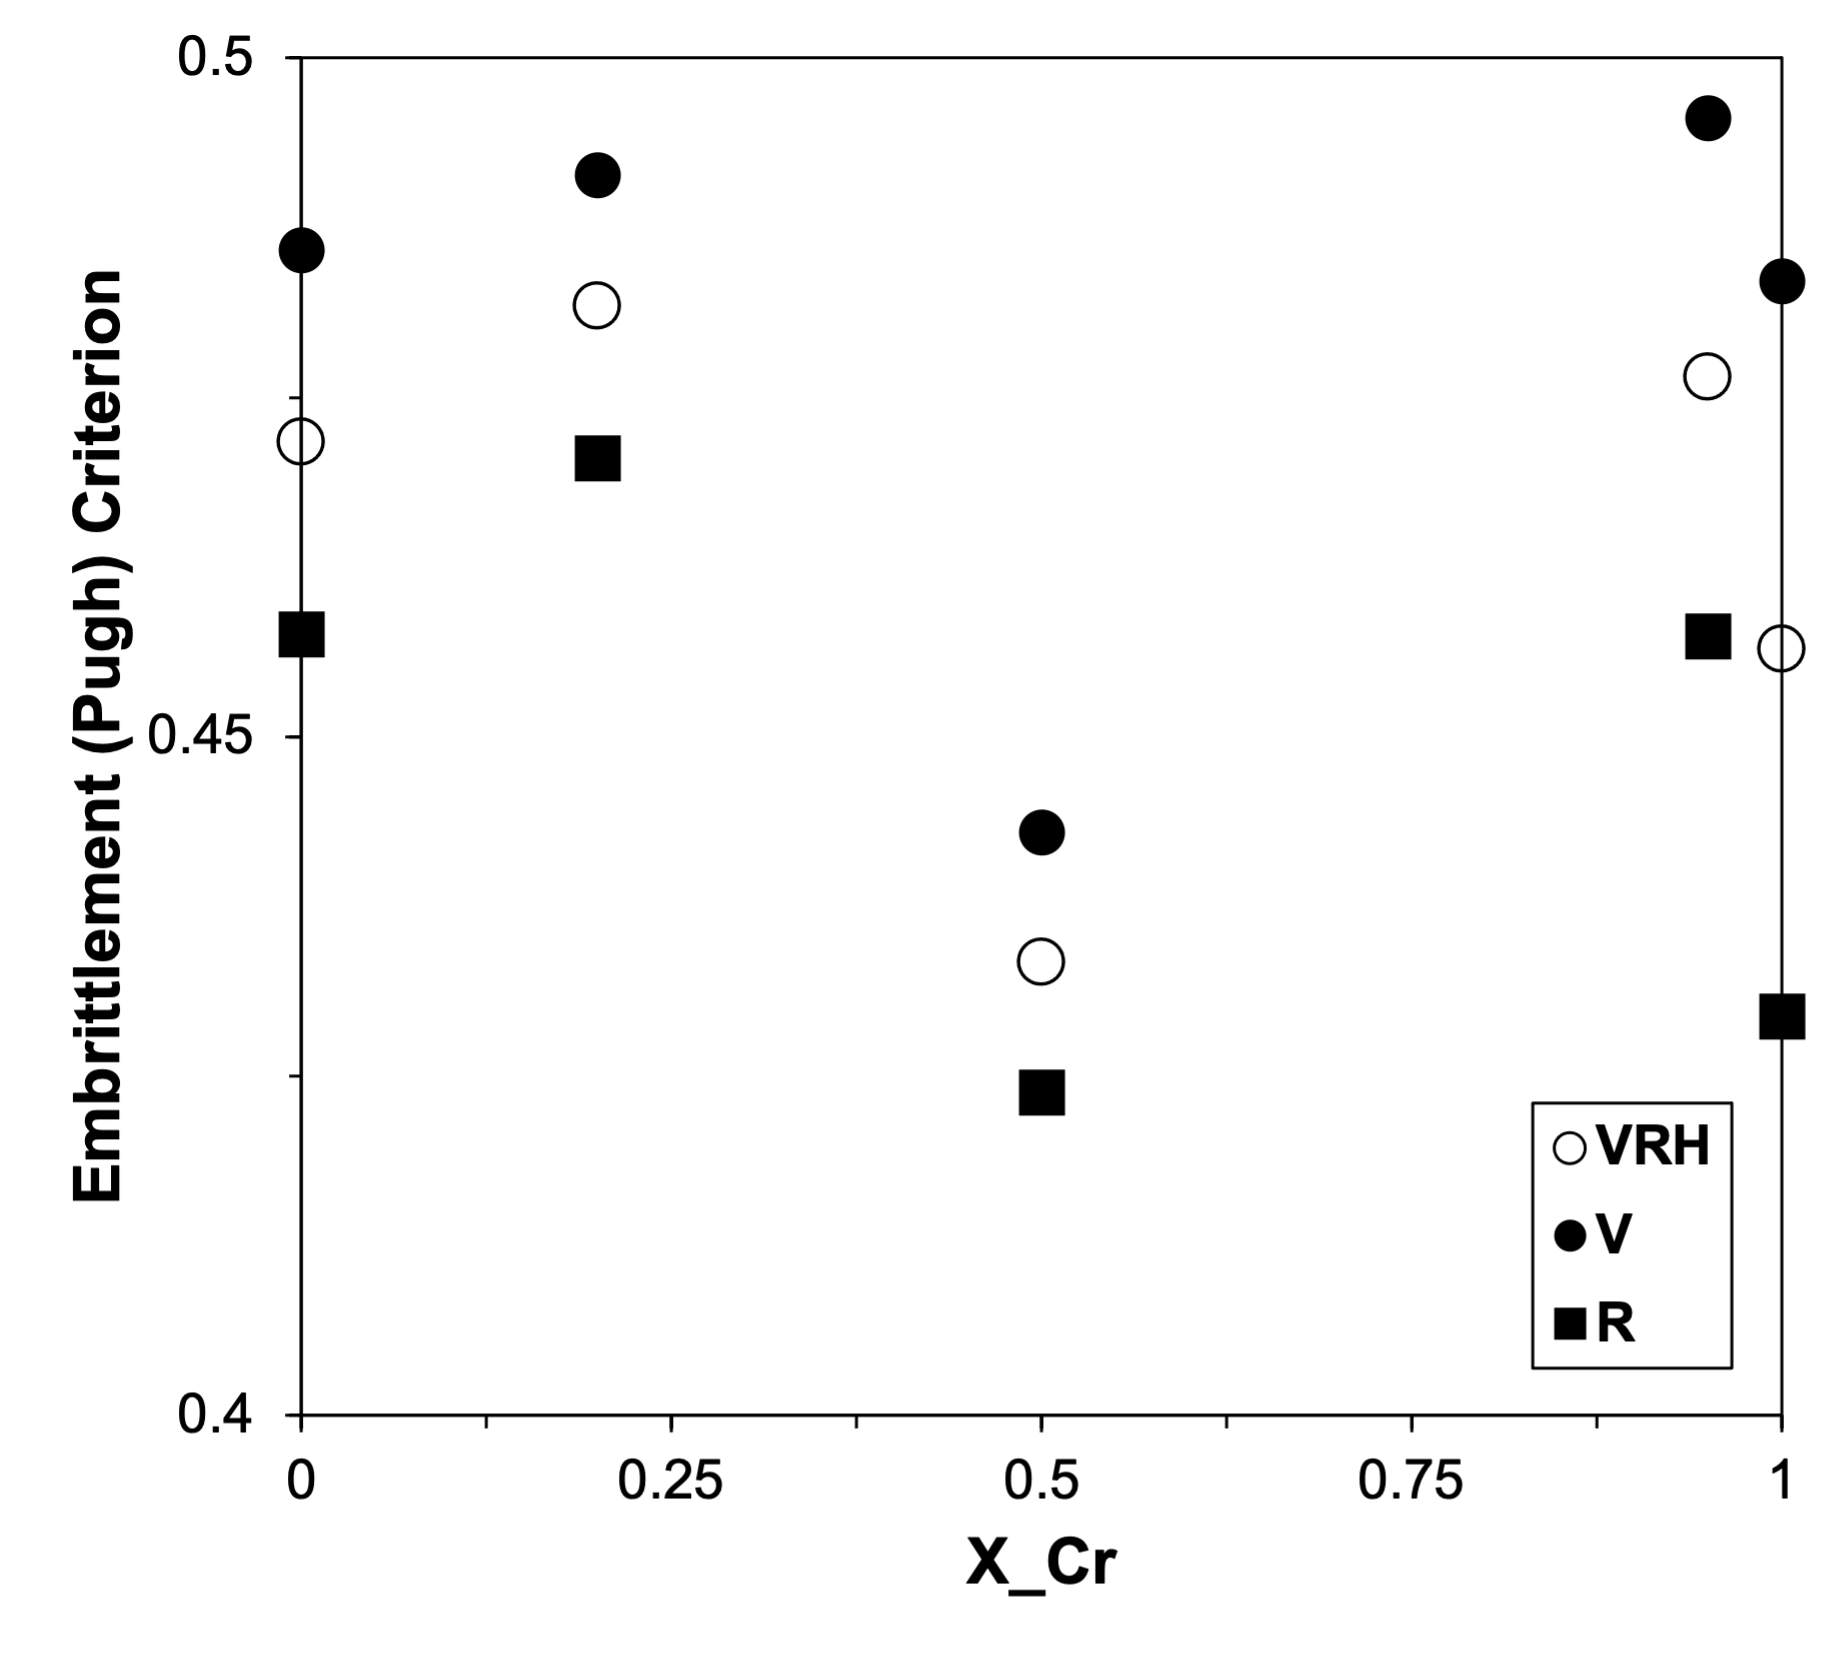
\includegraphics[width=\linewidth, right]{Parts/Figures/embrittlement-3.png}         \caption{Embrittlement (Pugh) Criterion}
         \label{fig1c}
     \end{subfigure}
	\caption{(a) Negative mixing enthalpy of Fe and Cr in a binary alloy indicate unmixing in the form of spinodal decomposition is thermodynamically favorable in bcc $\delta$-ferrite in cast austenitic stainless steels. The mixing enthalpy is calculated as difference between the \emph{ab initio} relaxation enthalpy of the binary alloy and the pure elements and verifies that the simulated alloys are under spinodal decomposition conditions. (c) Rayleigh wave frequency and (d) embrittlement (Pugh) criterion indicate spinodal decomposition-induced stiffening towards embrittlement. }
	\label{fig1}
\end{figure}
\end{comment}


\begin{figure}[!ht]
	\centering
	\begin{subfigure}{0.9\textwidth}
         \centering
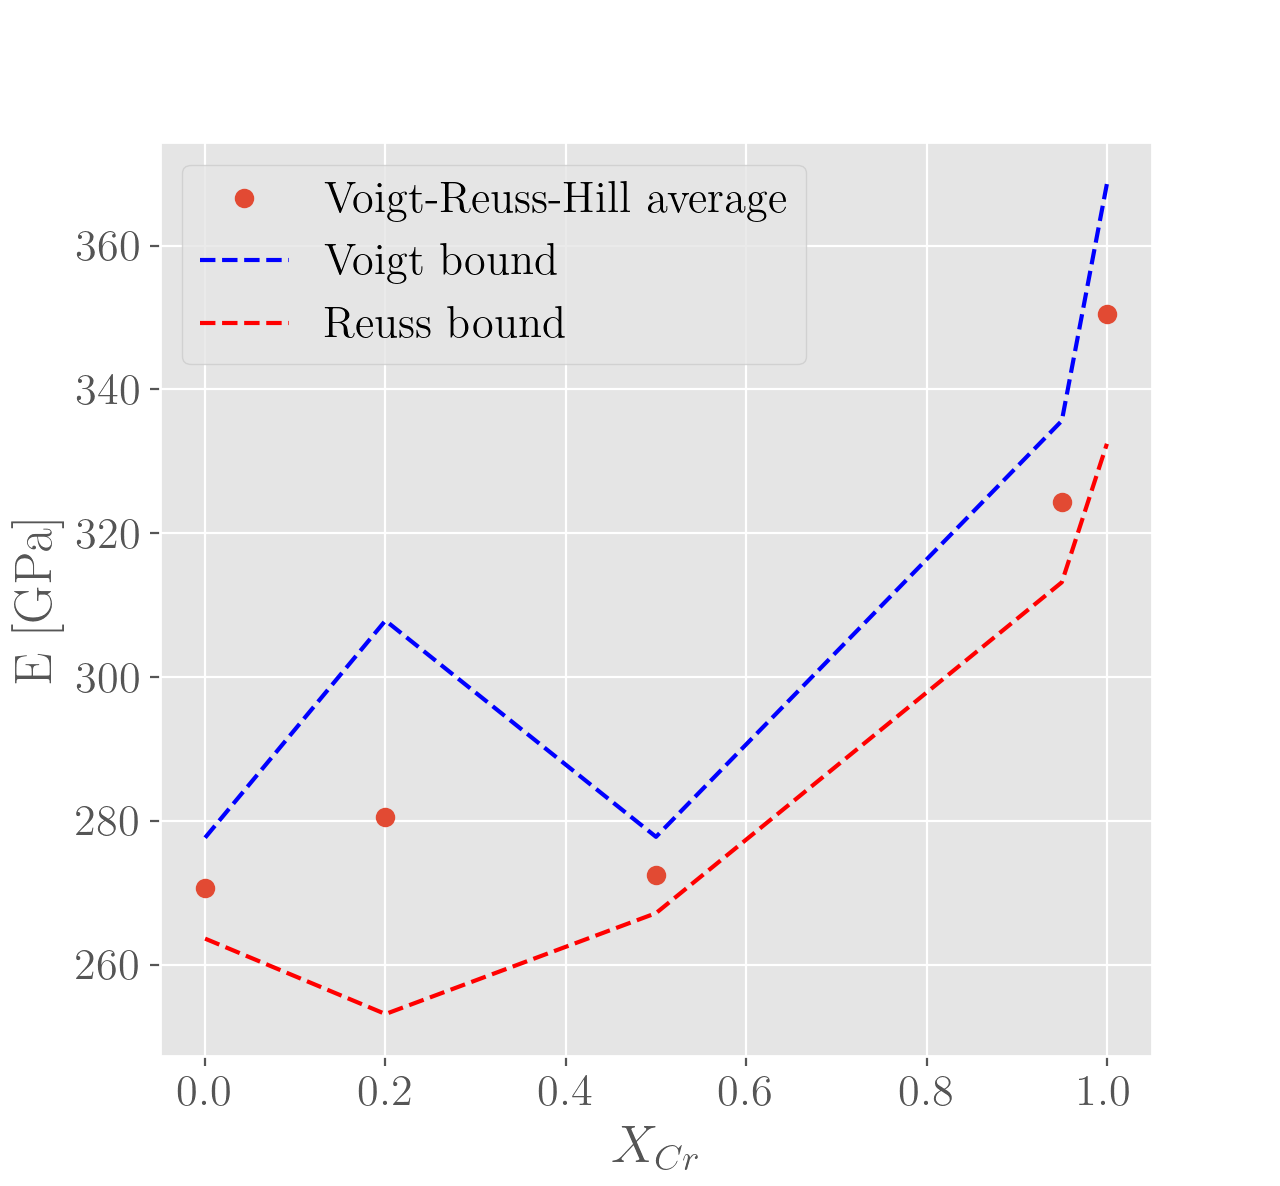
\includegraphics[width=\linewidth, left]{Parts/Figures/E_VRH.png}
         \caption{Elastic (Young's) Modulus, $E_{VRH}$}
         \label{fig2a}
     \end{subfigure}
     \hfill
     \begin{subfigure}{0.45\textwidth}
         \centering
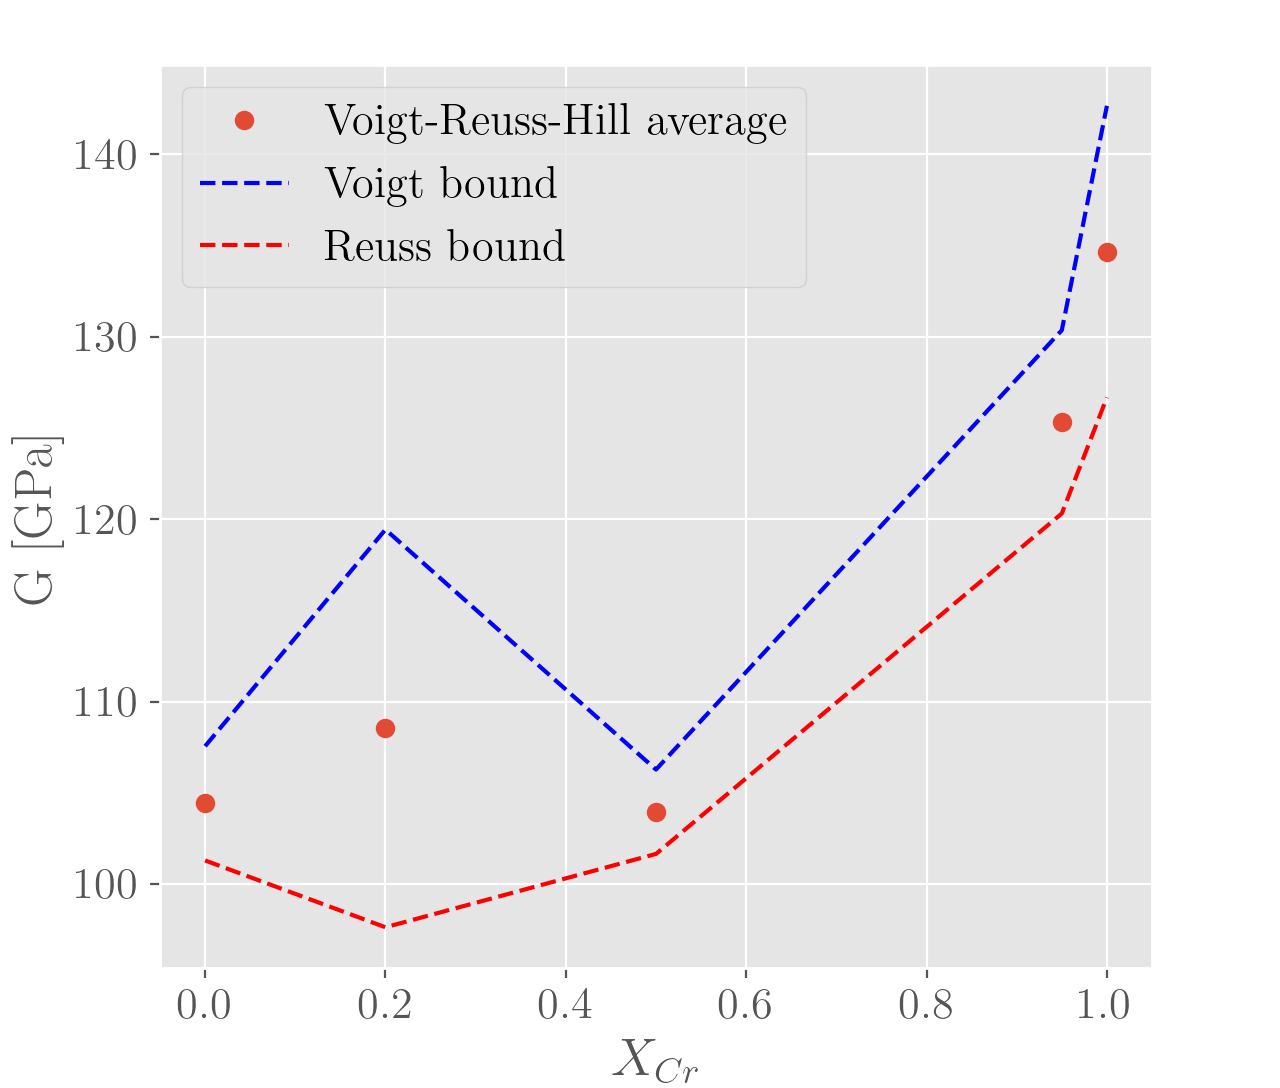
\includegraphics[width=\linewidth, right]{Parts/Figures/G_VRH.png}         \caption{Shear modulus, $G_{VRH}$ }
         \label{fig2b}
         \end{subfigure}
          \hfill
     \begin{subfigure}{0.45\textwidth}
         \centering
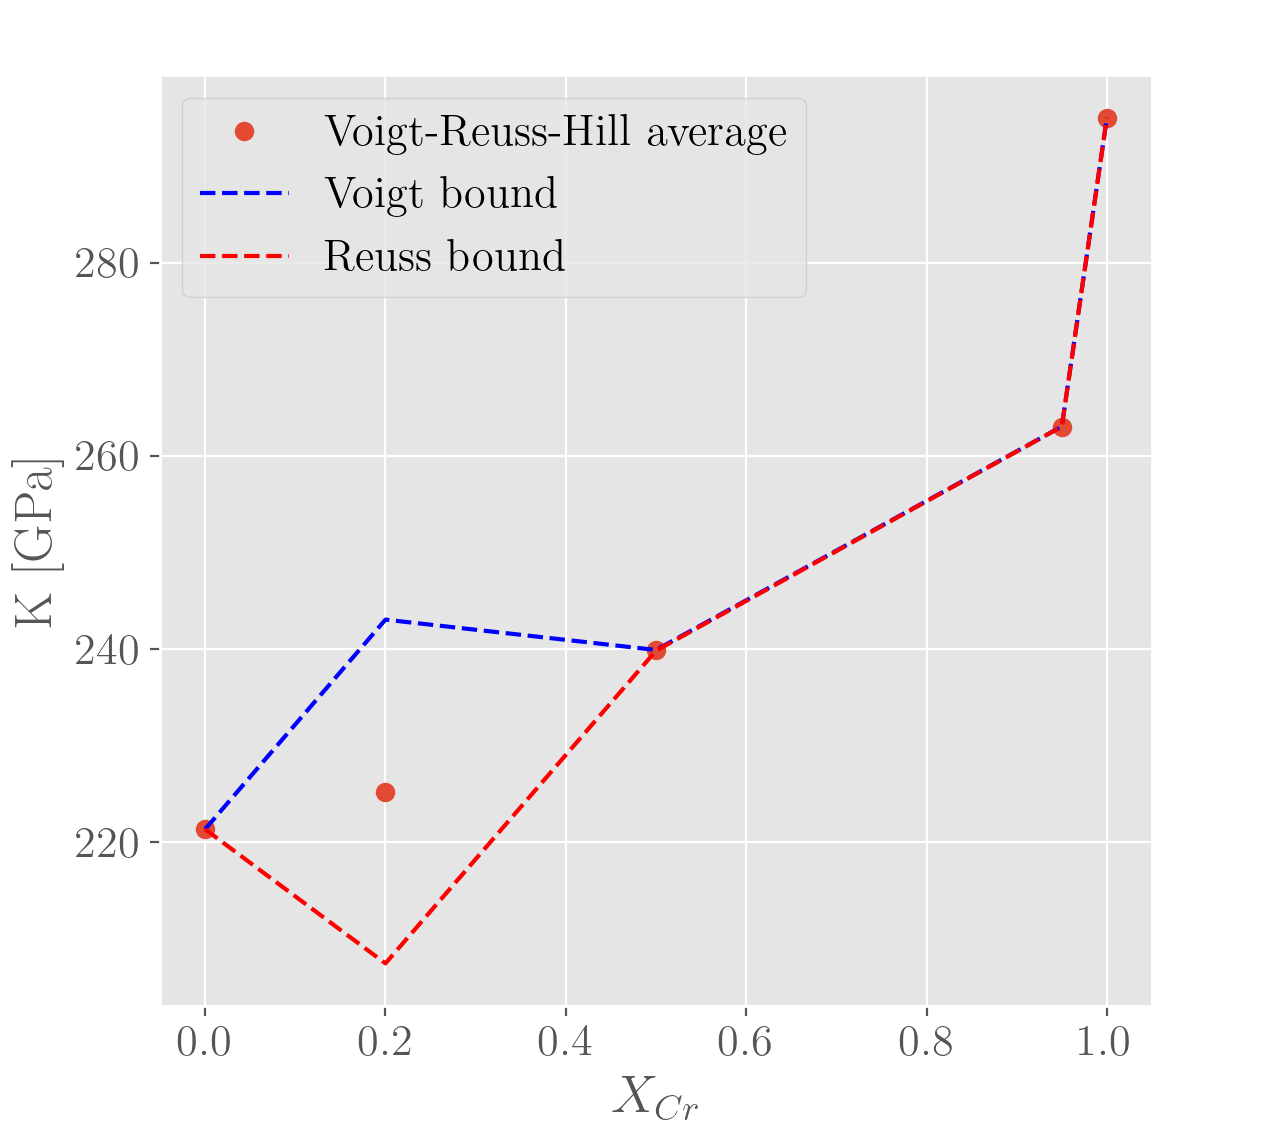
\includegraphics[width=\linewidth, right]{Parts/Figures/K_VRH.png}         \caption{Bulk modulus, $K_{VRH}$}
         \label{fig2c}
     \end{subfigure}
	\caption{Elastic moduli of bcc binary FeCr as a function of Cr composition indicate spinodal decomposition-induced stiffening towards embrittlement. The trends and values are consistent with theoretical and experimental results reported in literature. [REF] (a) ... (b) ... (c) ...}
	\label{fig2}
\end{figure}

\begin{sidewaysfigure}[!ht]
	\centering
	\begin{subfigure}{0.7\textwidth}
         \centering
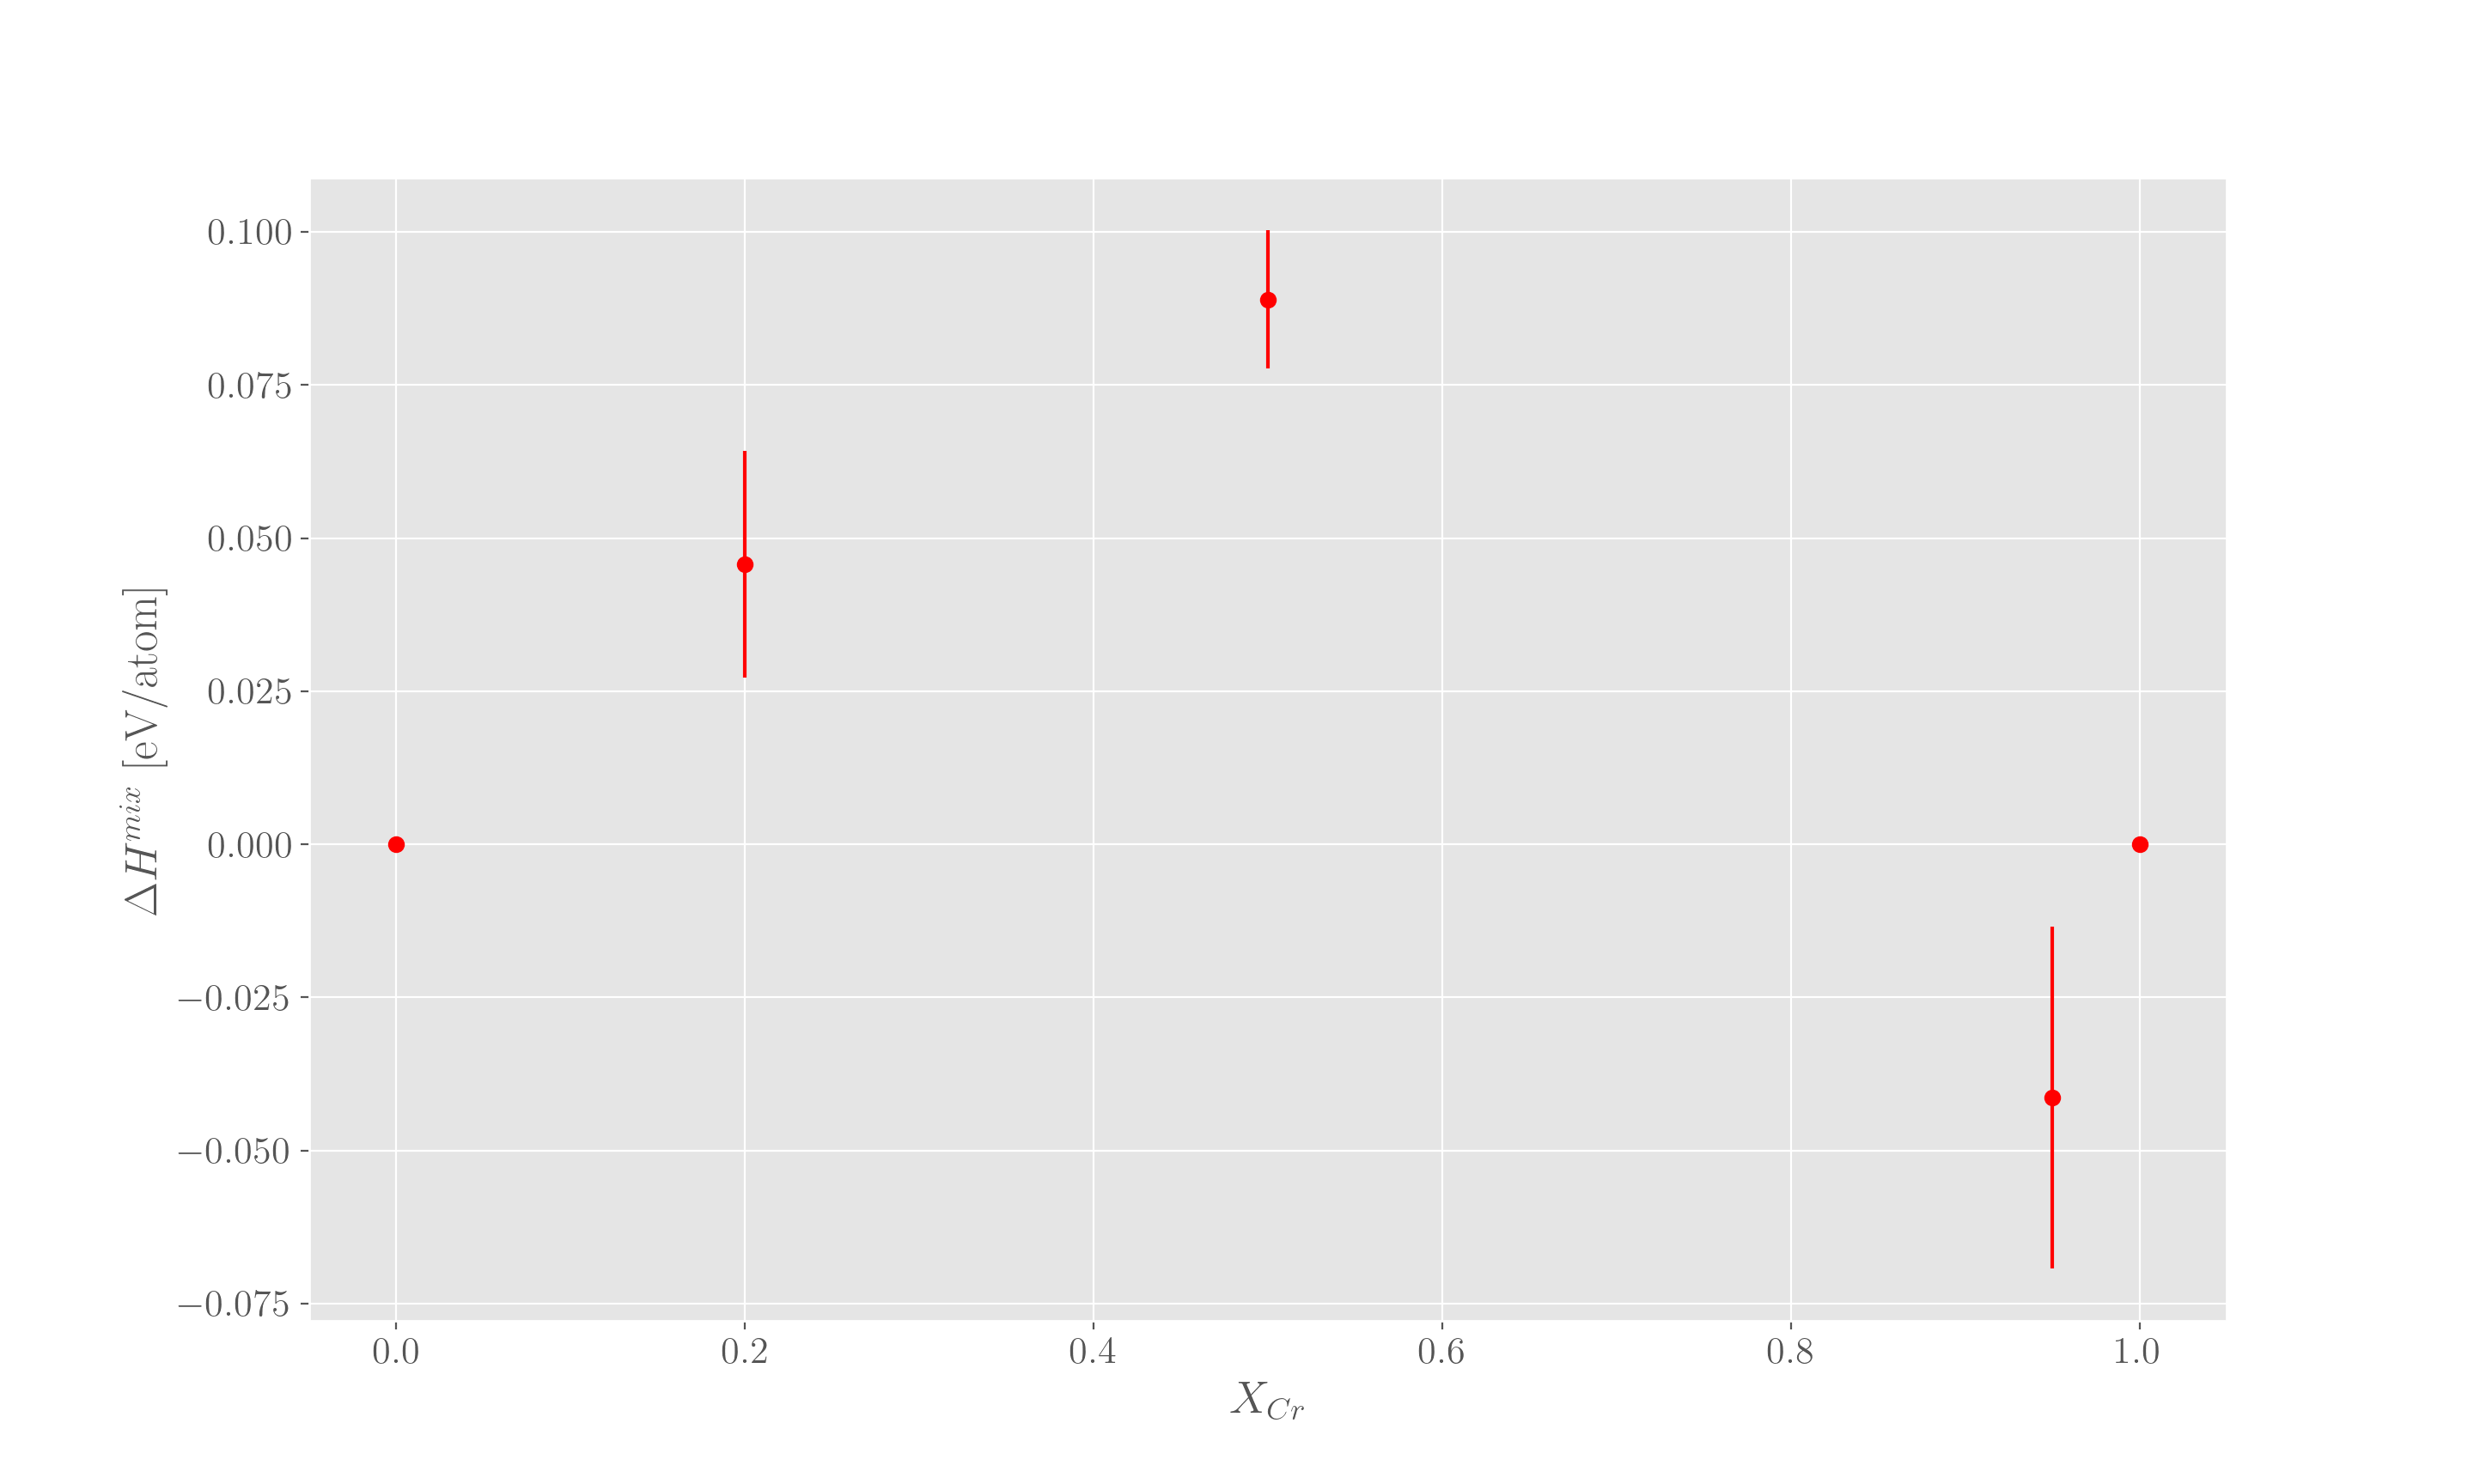
\includegraphics[width=\linewidth, left]{Parts/Figures/Hmix-vF.png}
         \caption{Enthalpy of mixing}
         \label{fig3a}
     \end{subfigure}
          \begin{subfigure}{0.3\textwidth}
         \centering
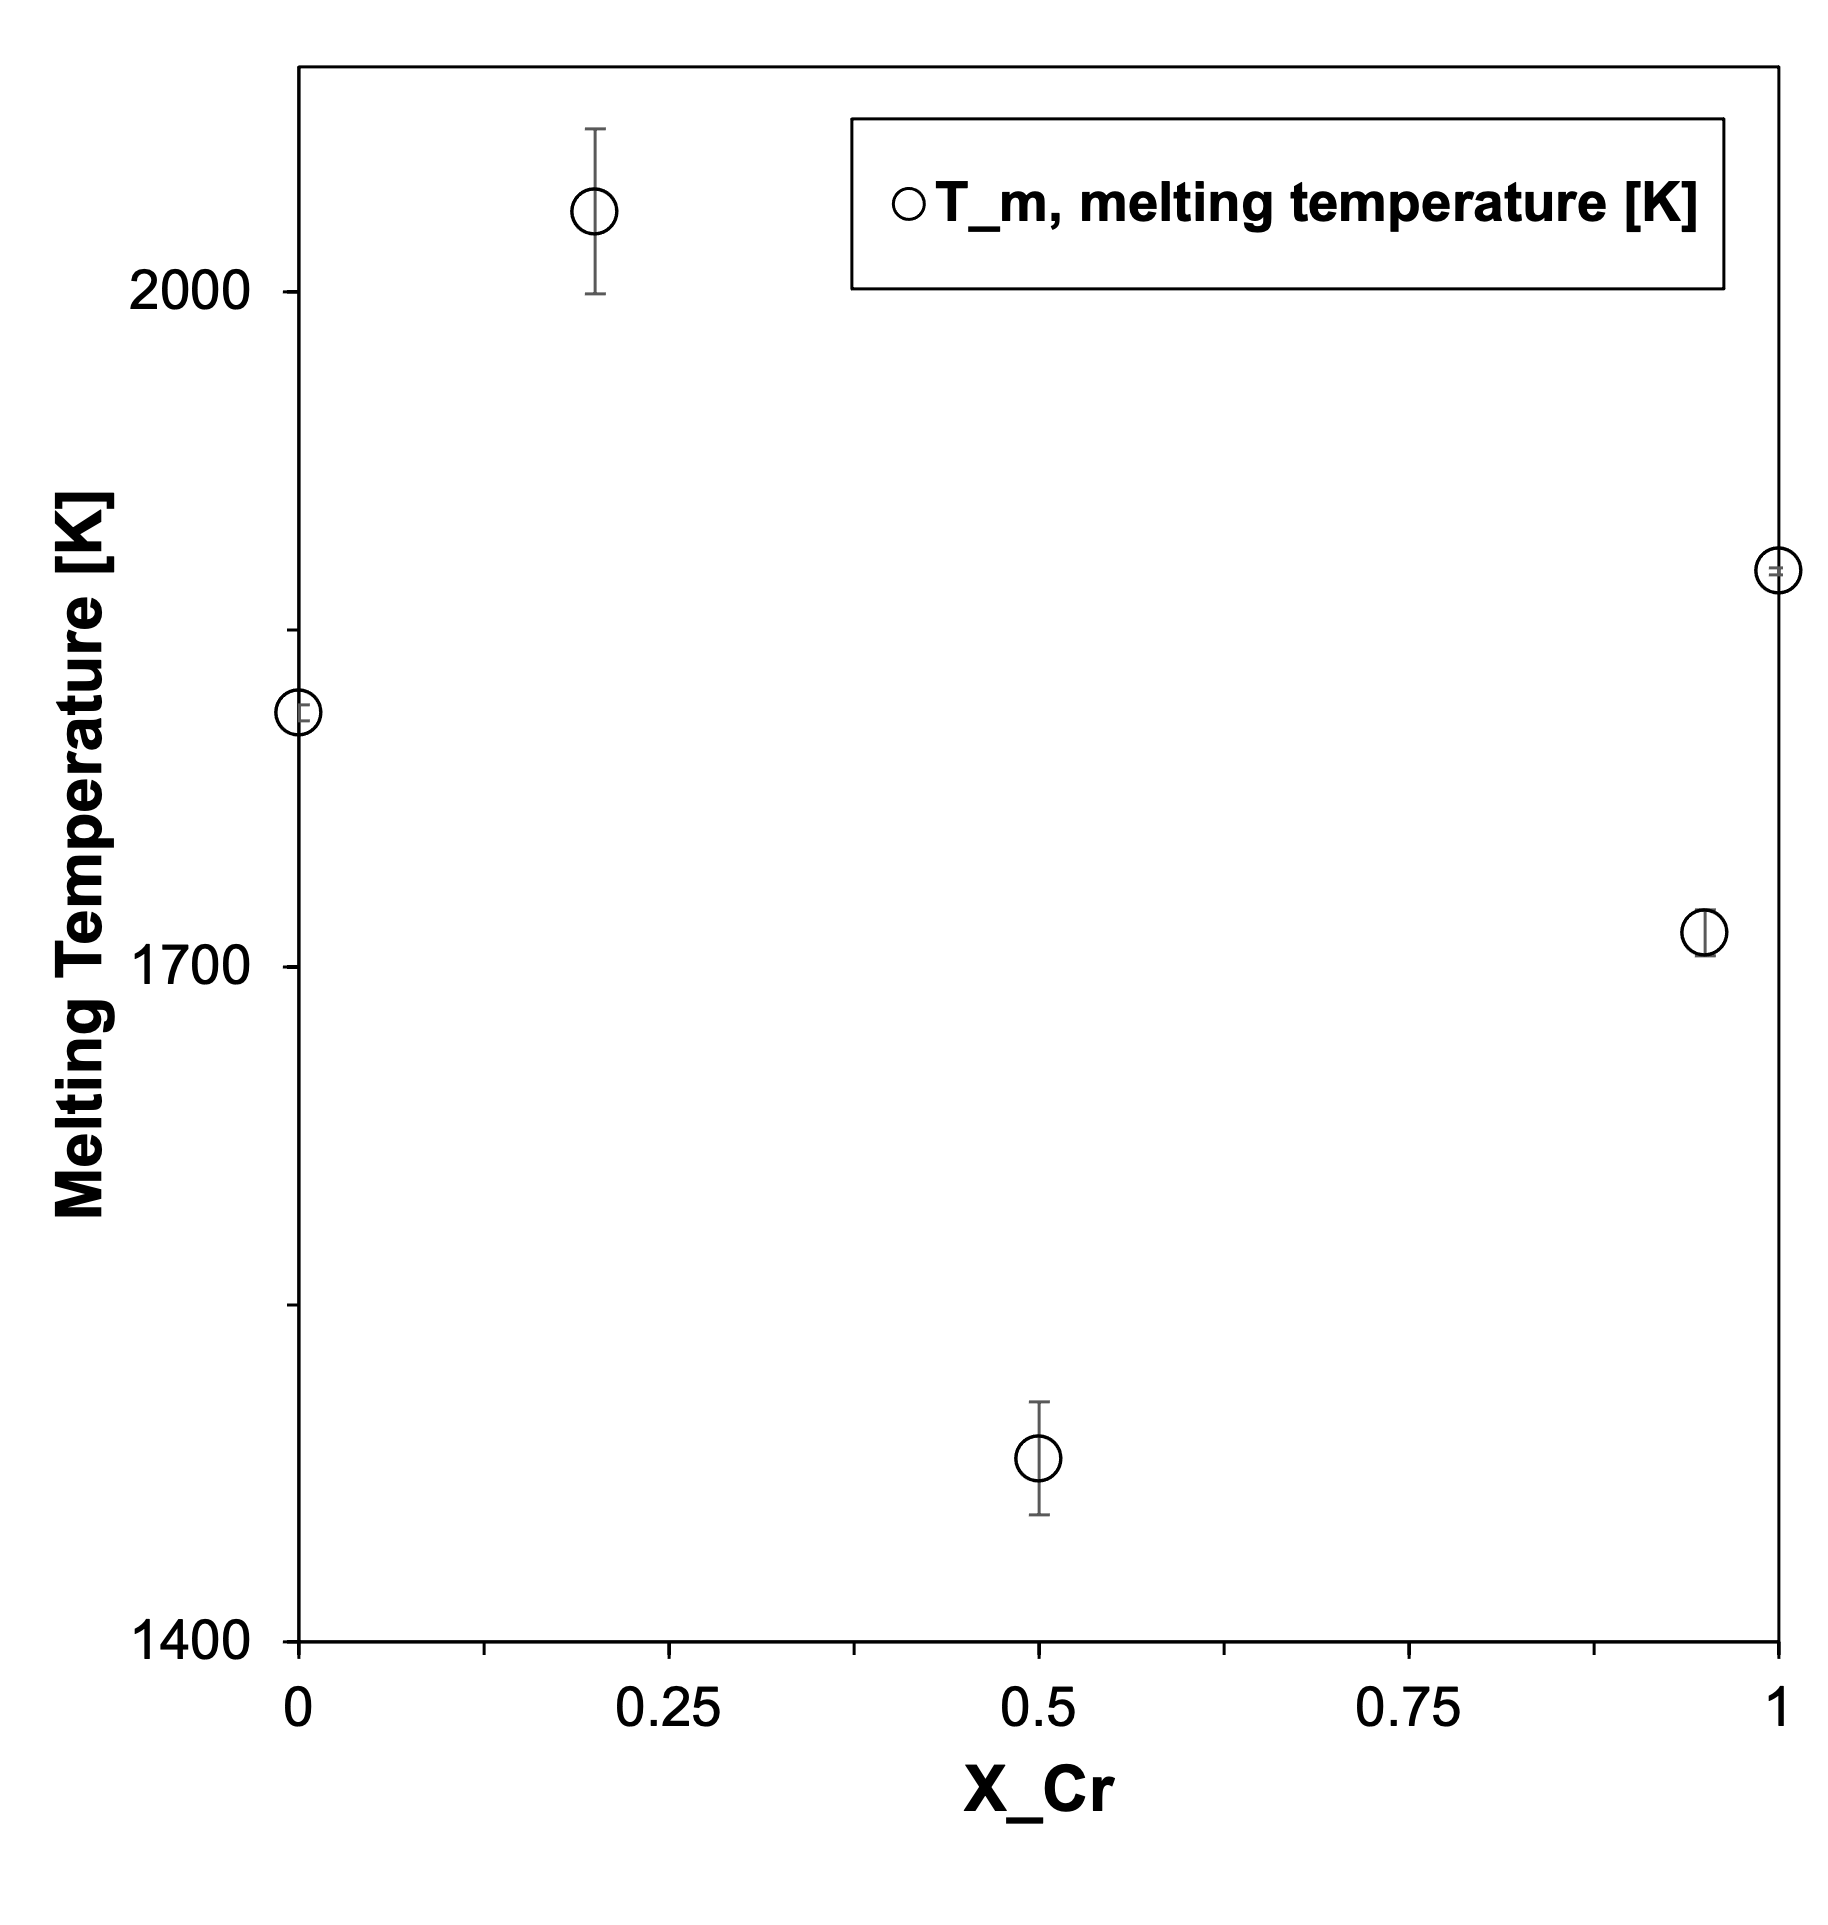
\includegraphics[width=\linewidth, right]{Parts/Figures/TMvsX_v2.png}         \caption{$T_M$, melting temperature}
         \label{fig3b}
     \end{subfigure}
     \begin{subfigure}{0.3\textwidth}
         \centering
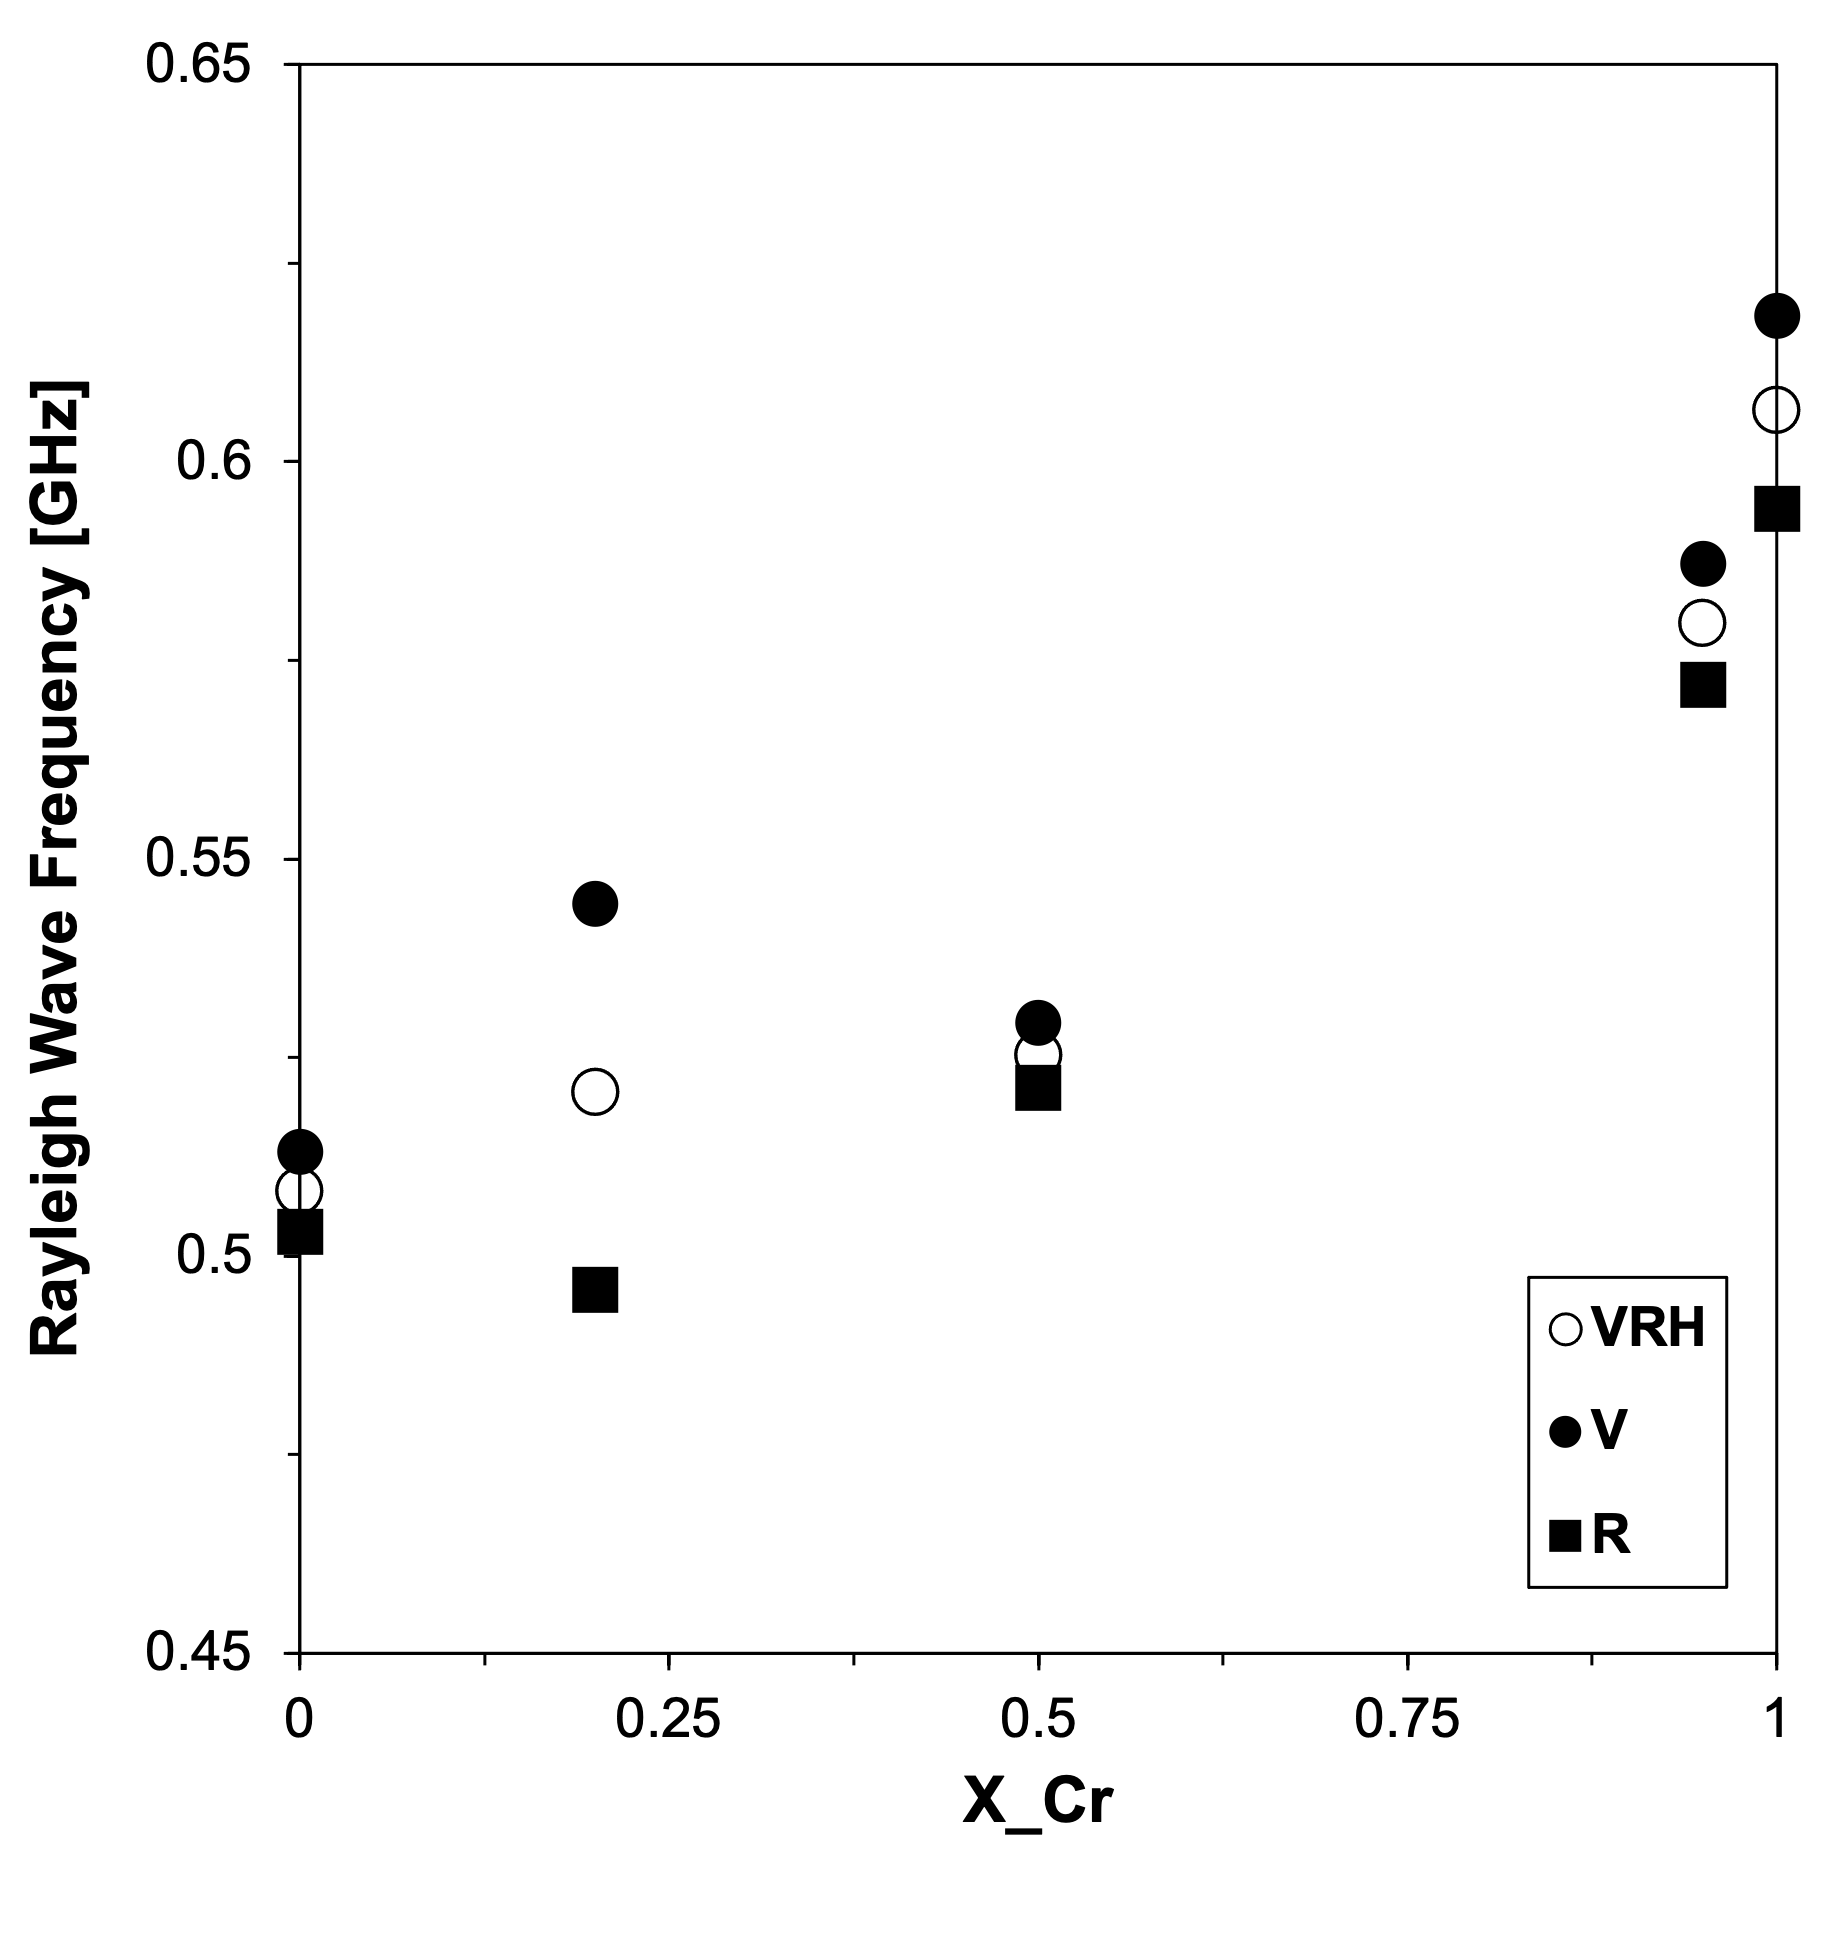
\includegraphics[width=\linewidth, right]{Parts/Figures/f_rwVsX_vF.png}         \caption{Rayleigh wave frequencies}
         \label{fig3c}
         \end{subfigure}
     \begin{subfigure}{0.3\textwidth}
         \centering
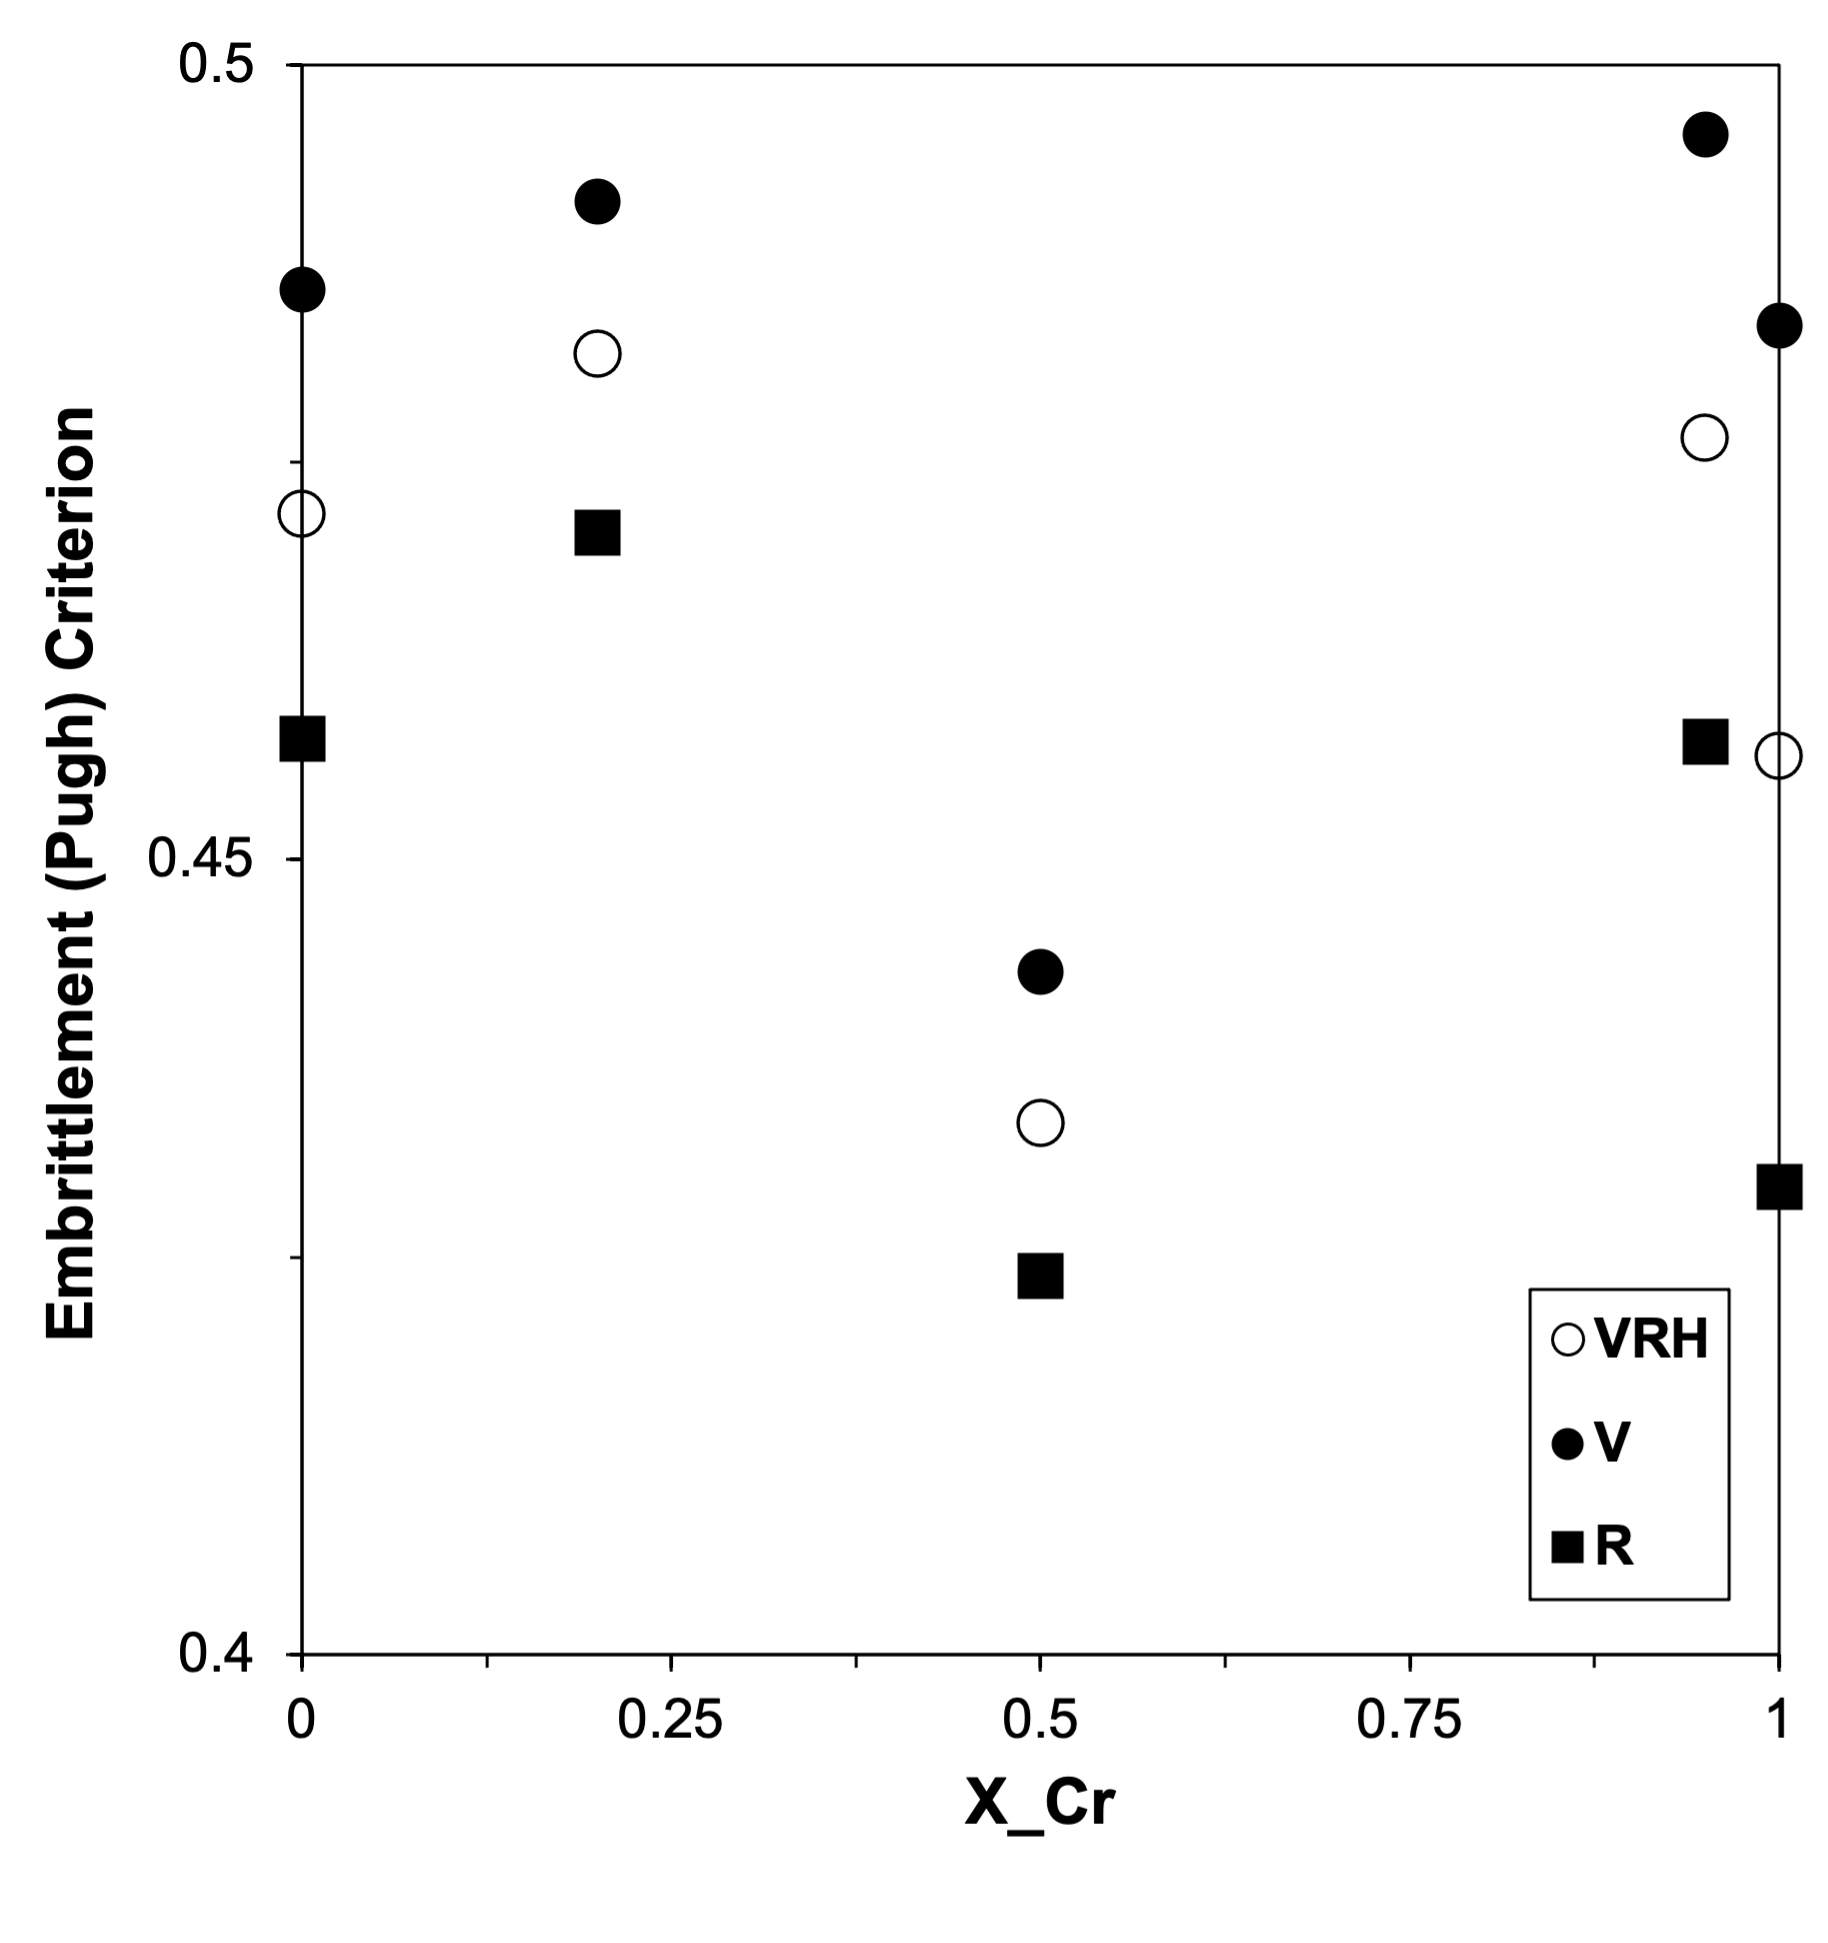
\includegraphics[width=\linewidth, right]{Parts/Figures/EvsX_vF.png}         \caption{Embrittlement (Pugh) Criterion}
         \label{fig3d}
     \end{subfigure}
	\caption{(a) Negative mixing enthalpy of Fe and Cr in a binary alloy indicate unmixing in the form of spinodal decomposition is thermodynamically favorable in bcc $\delta$-ferrite in cast austenitic stainless steels. The mixing enthalpy is calculated as difference between the \emph{ab initio} relaxation enthalpy of the binary alloy and the pure elements and verifies that the simulated alloys are under spinodal decomposition conditions. (b) Melting temperature as a function of Cr composition confirms elasticity could be related to plasticity. \cite{pugh1954xcii} (c) Rayleigh wave frequency as a function of Cr compositions verifies spinodal decomposition-induced stiffening as a result of separation of bcc $\delta$-ferrite into Fe-rich/Cr-depleted Cr-rich/Fe-depleted regions and (d) embrittlement (Pugh) criterion calculated for these compositions indicate spinodal decomposition-induced stiffening towards embrittlement. }
	\label{fig2}
\end{sidewaysfigure}




\begin{comment}
    
\begin{figure}[!ht]
	\centering
	\begin{subfigure}{0.45\textwidth}
         \centering
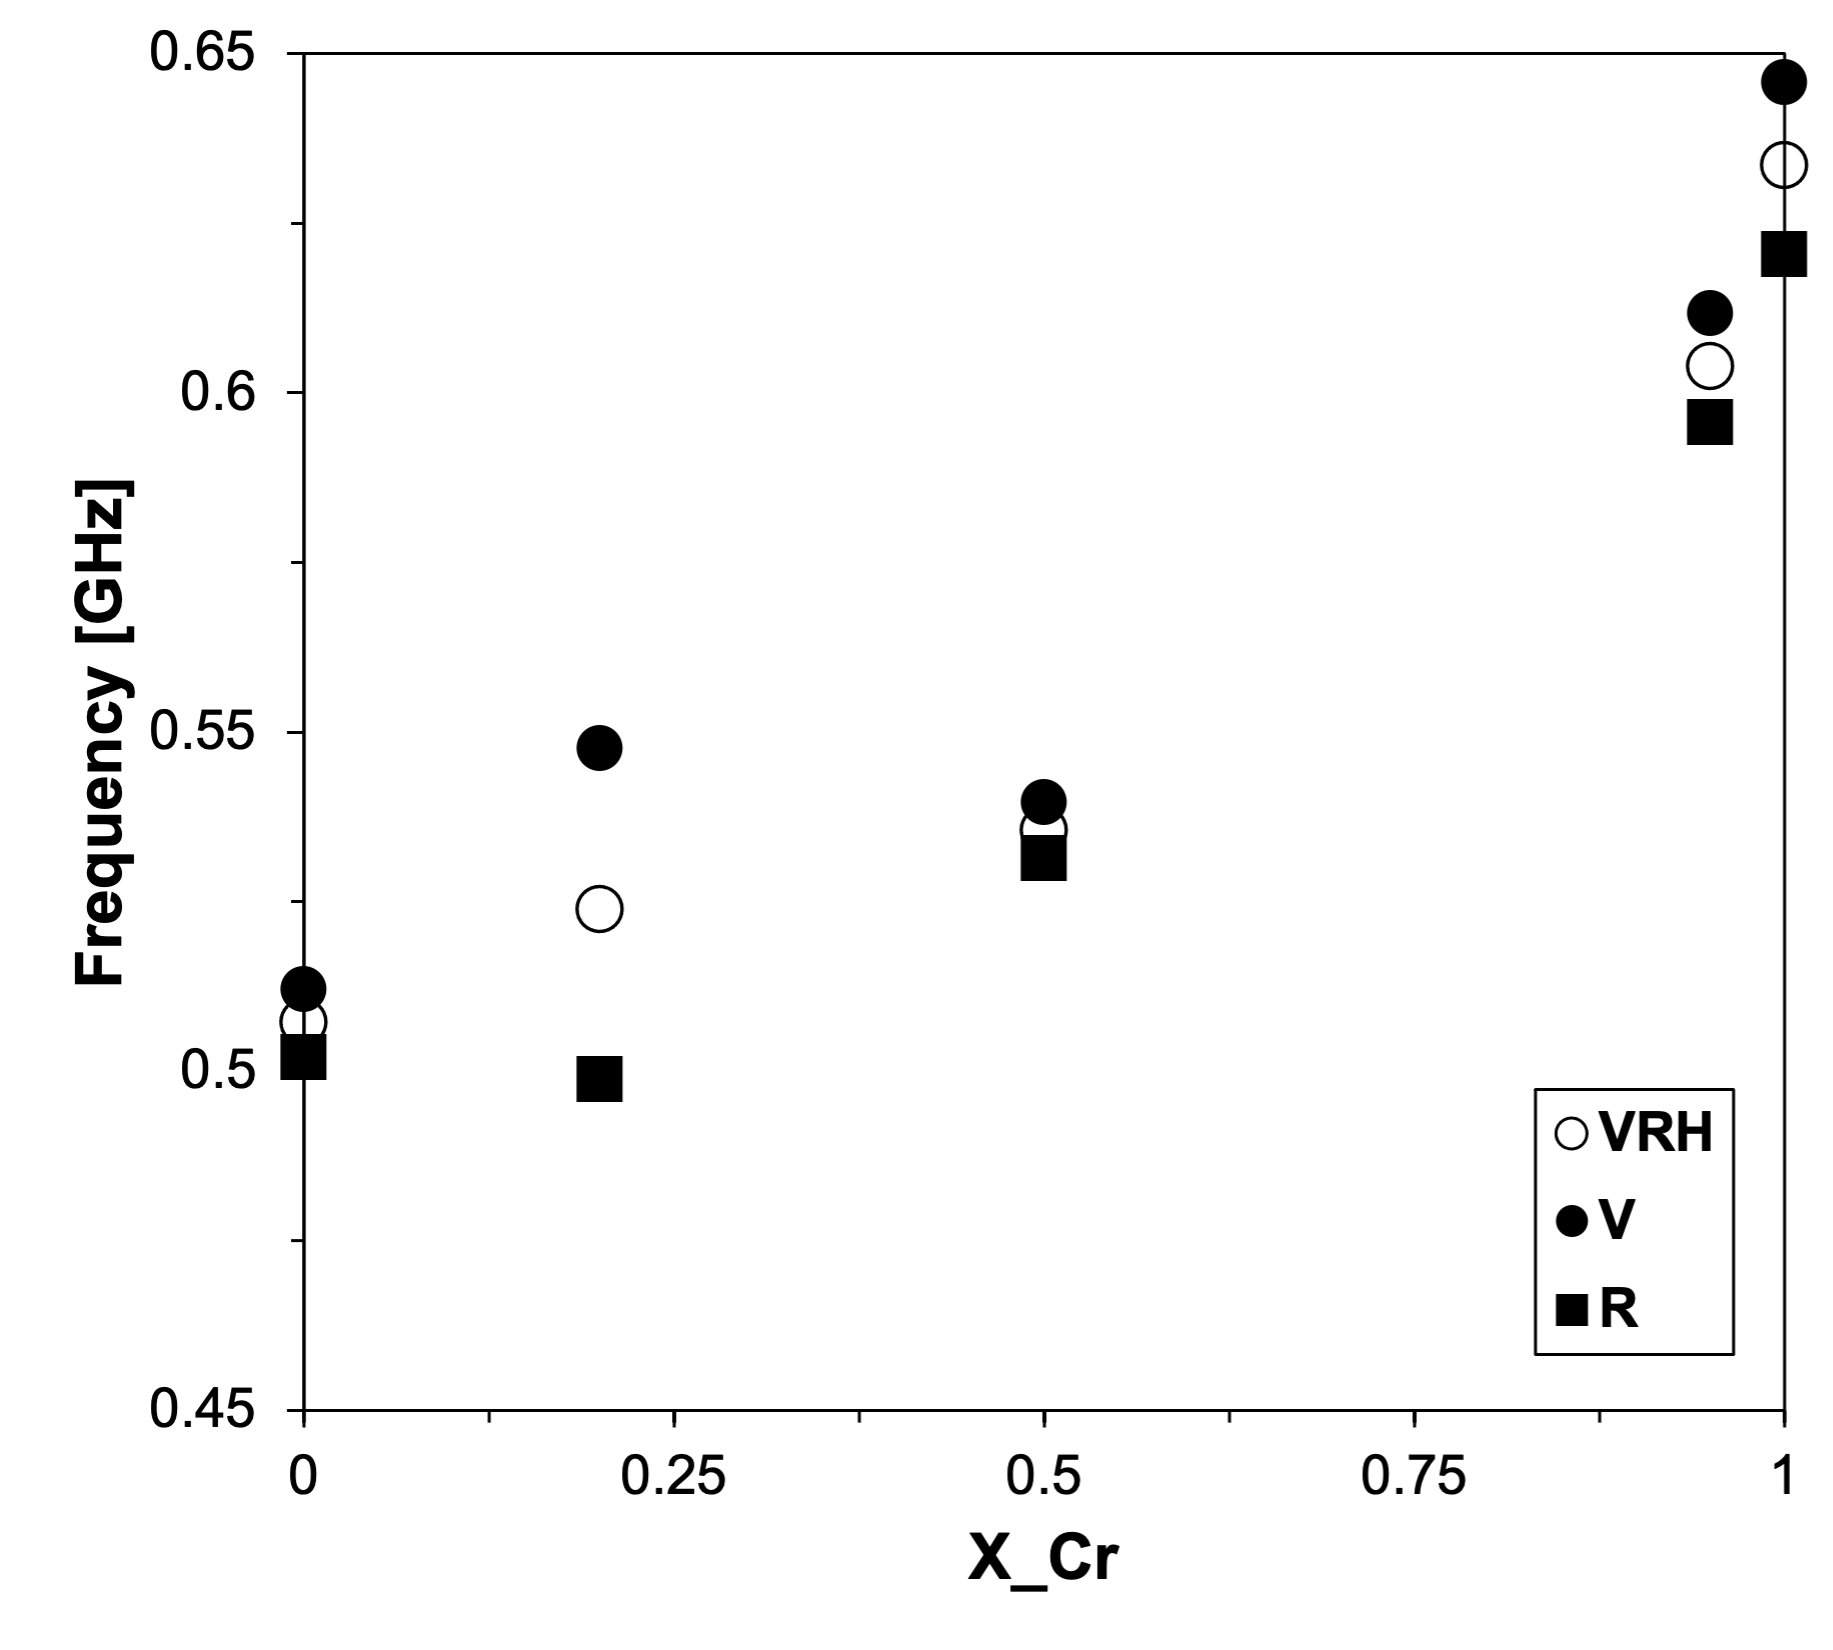
\includegraphics[width=\linewidth, left]{Parts/Figures/rayleigh-wave-3.png}
         \caption{Stiffening predictions}
         \label{fig4a}
     \end{subfigure}
     \hfill
     \begin{subfigure}{0.45\textwidth}
         \centering
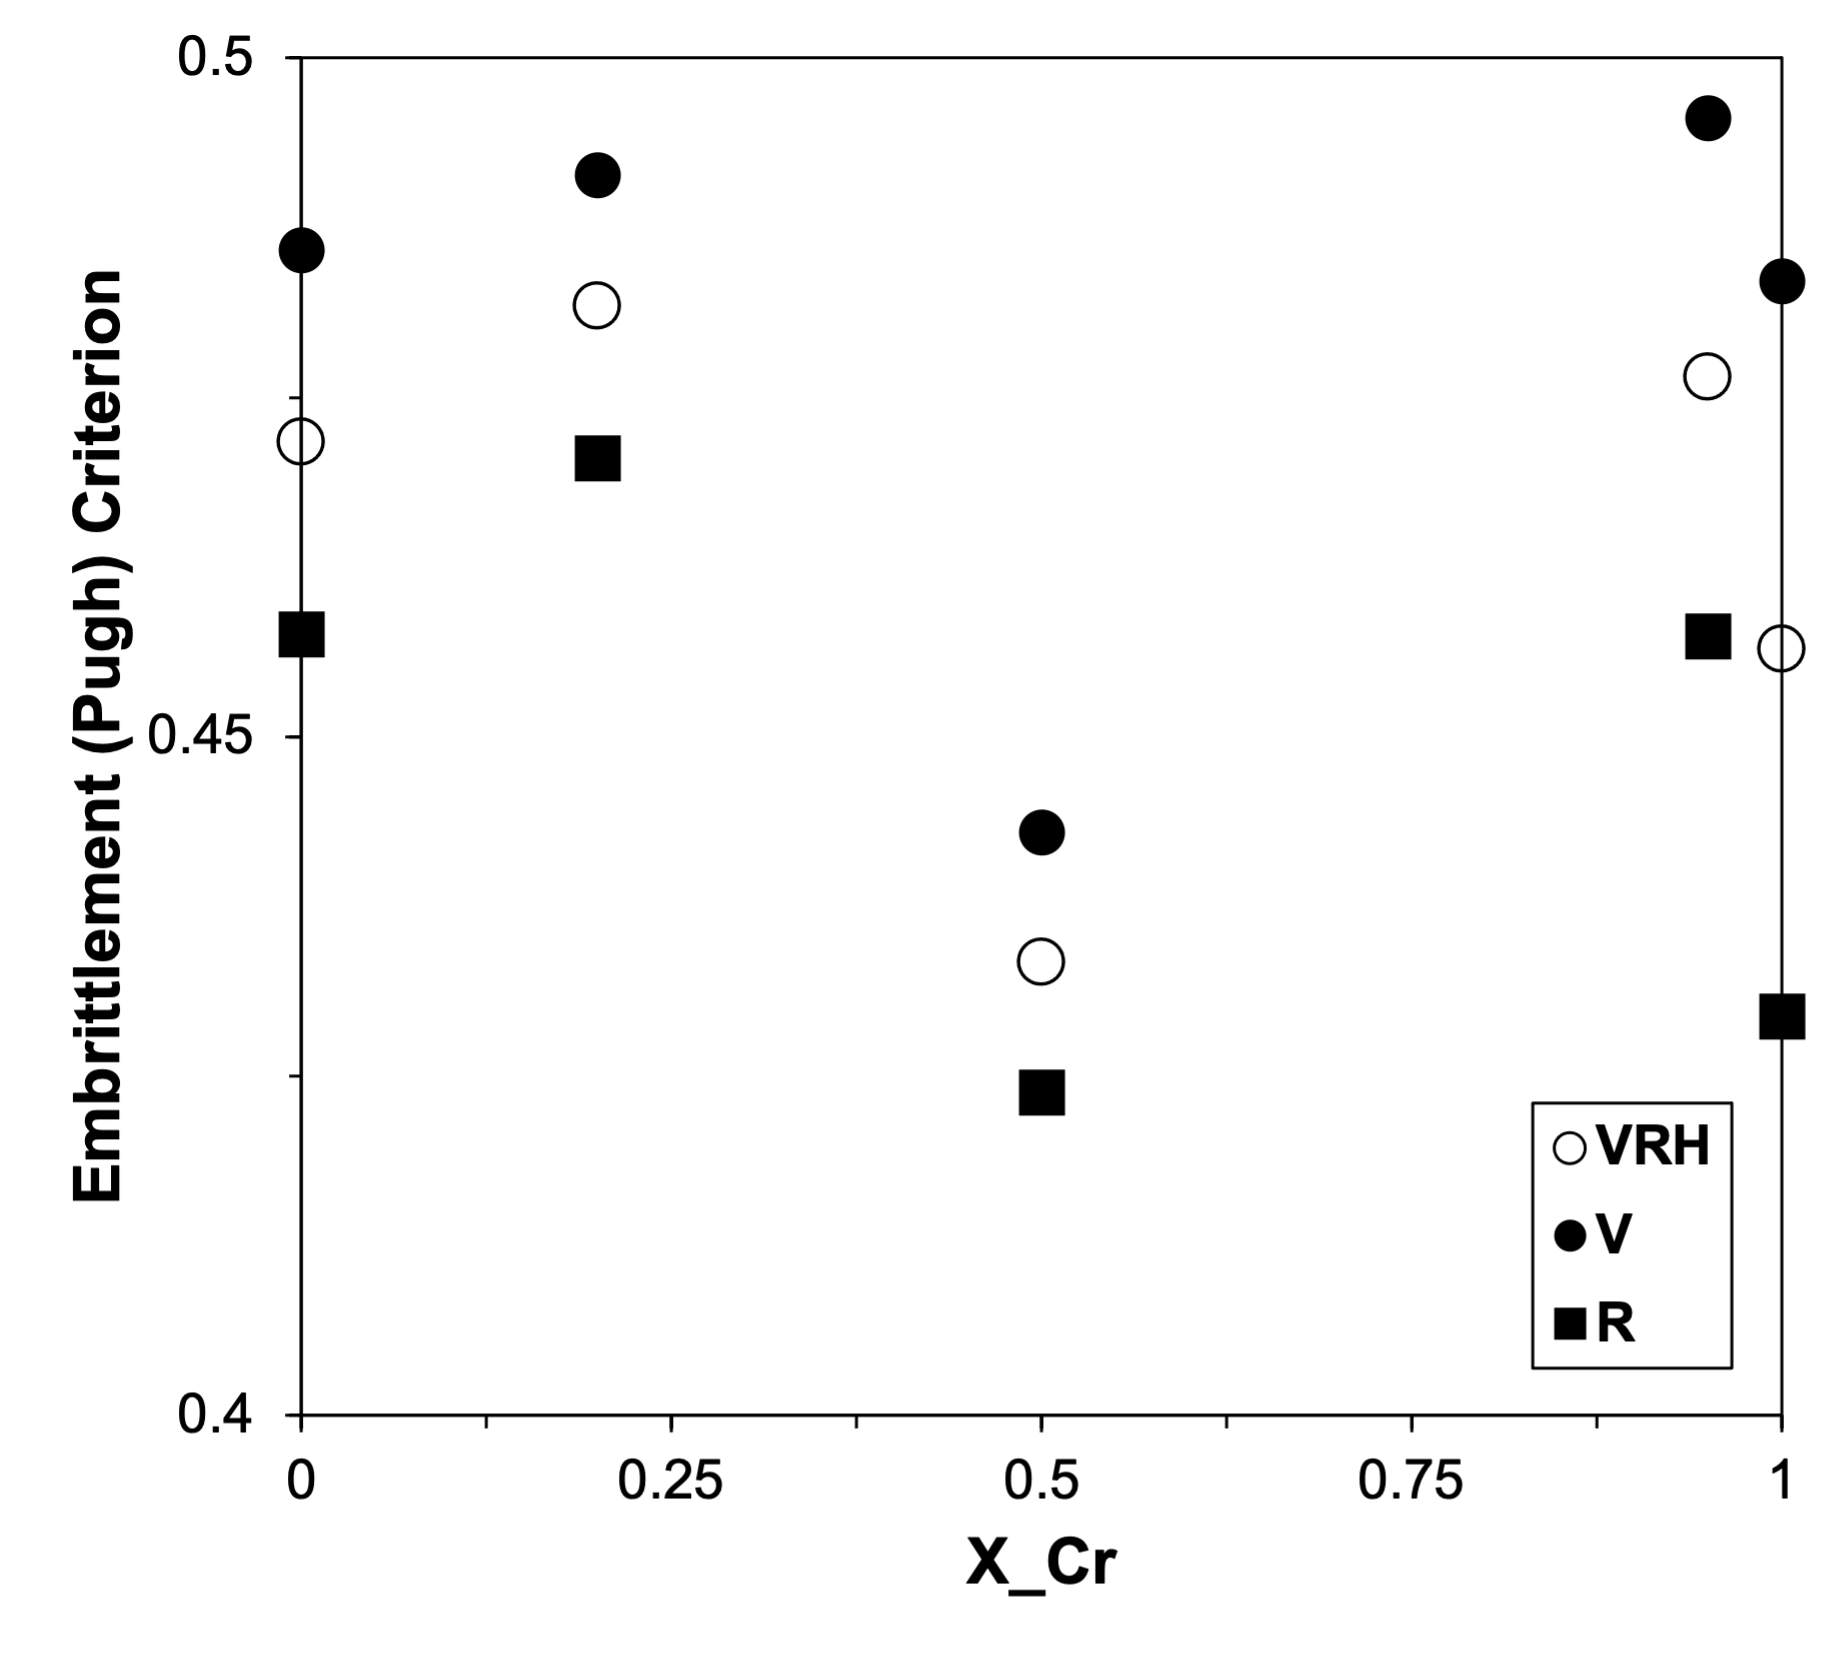
\includegraphics[width=\linewidth, right]{Parts/Figures/embrittlement-3.png}         \caption{Embrittlement predictions}
         \label{fig4b}
     \end{subfigure}
	\caption{Rayleigh wave frequency and embrittlement (Pugh) criterion indicate spinodal decomposition-induced stiffening towards embrittlement. (a) ... (b) ... }
	\label{fig4}
\end{figure}
\end{comment}


\begin{comment}
\begin{figure}[!ht]
    \centering
    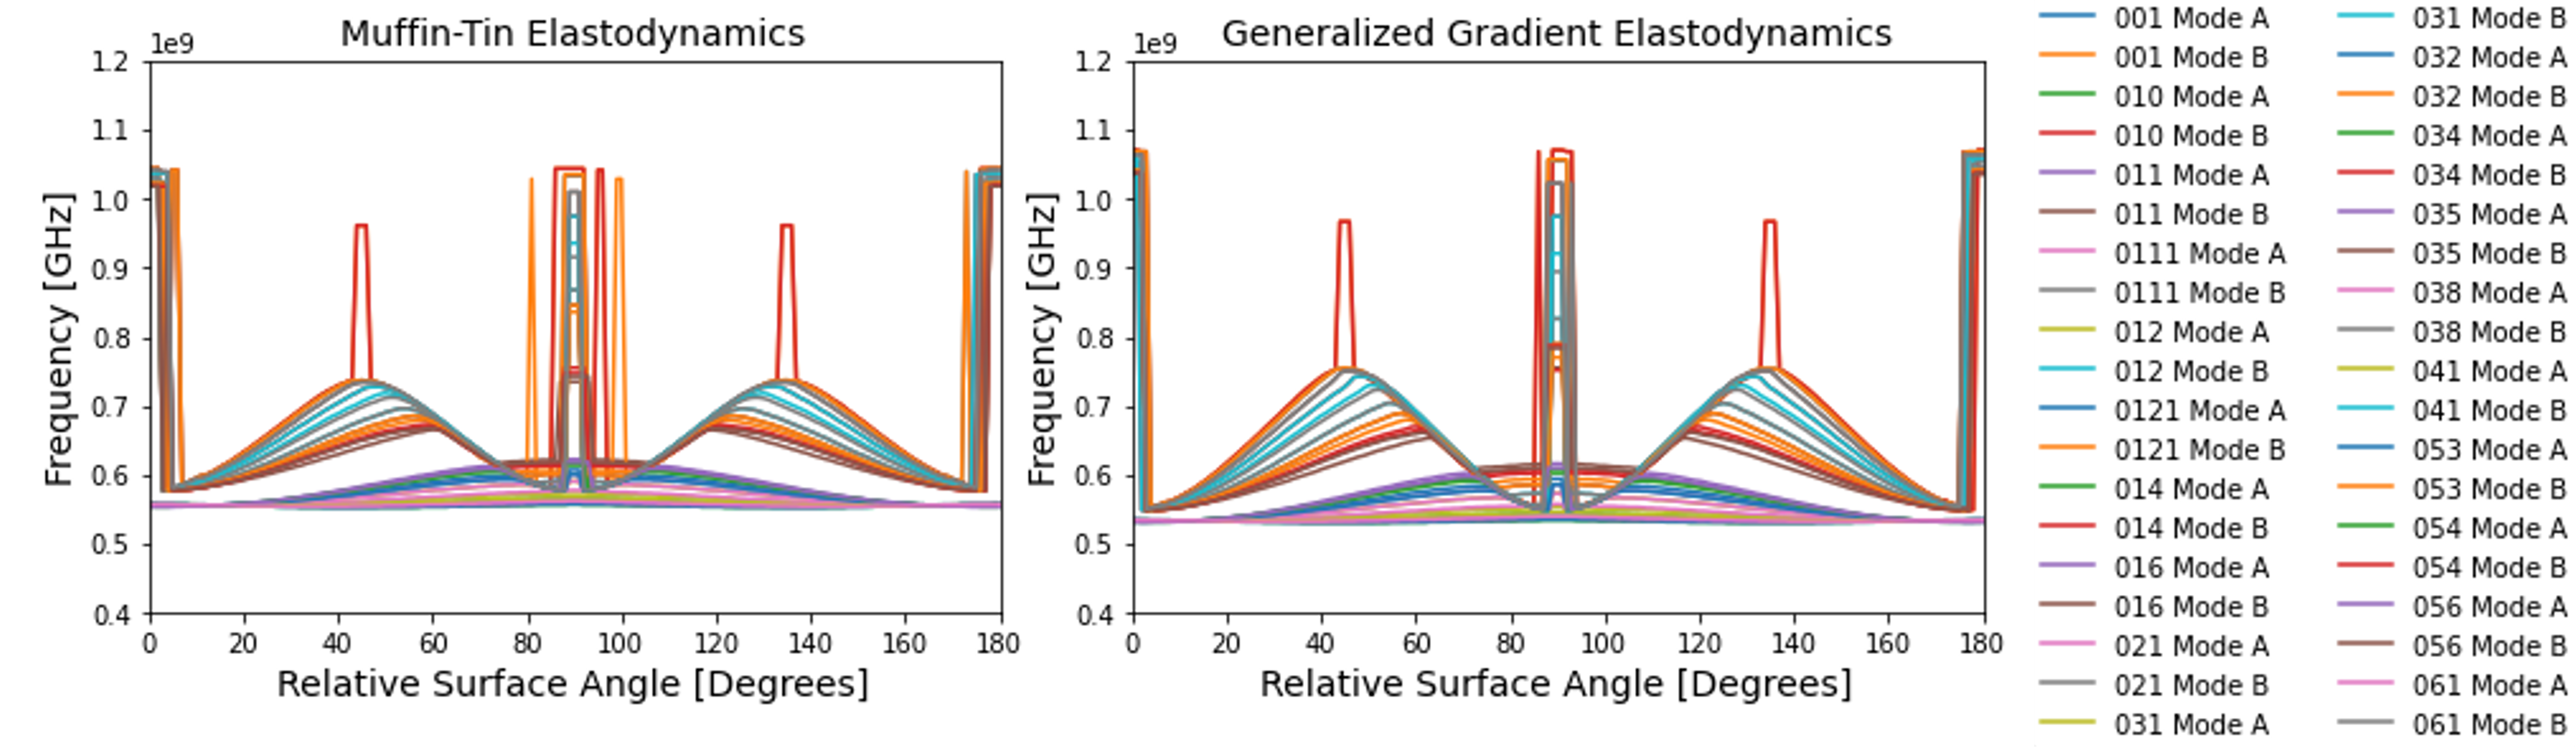
\includegraphics[width=\textwidth]{Parts/Figures/smoking-gun-v2.png}
    \caption{Quantum elastodynamic frequencies as calculated from the muffin-tin approximation and generalized gradient approximation of the ionic potential in density functional theory reveal new modes in the elastodynamically-unallowed region predicted in pristine stainless steel, and match experimentally-measured values in stainless steels that have undergone spinodal decomposition. [REF]}
    \label{fig5}
\end{figure}
\end{comment}






\begin{comment}
    \begin{sidewaysfigure}[!ht]
    \centering

    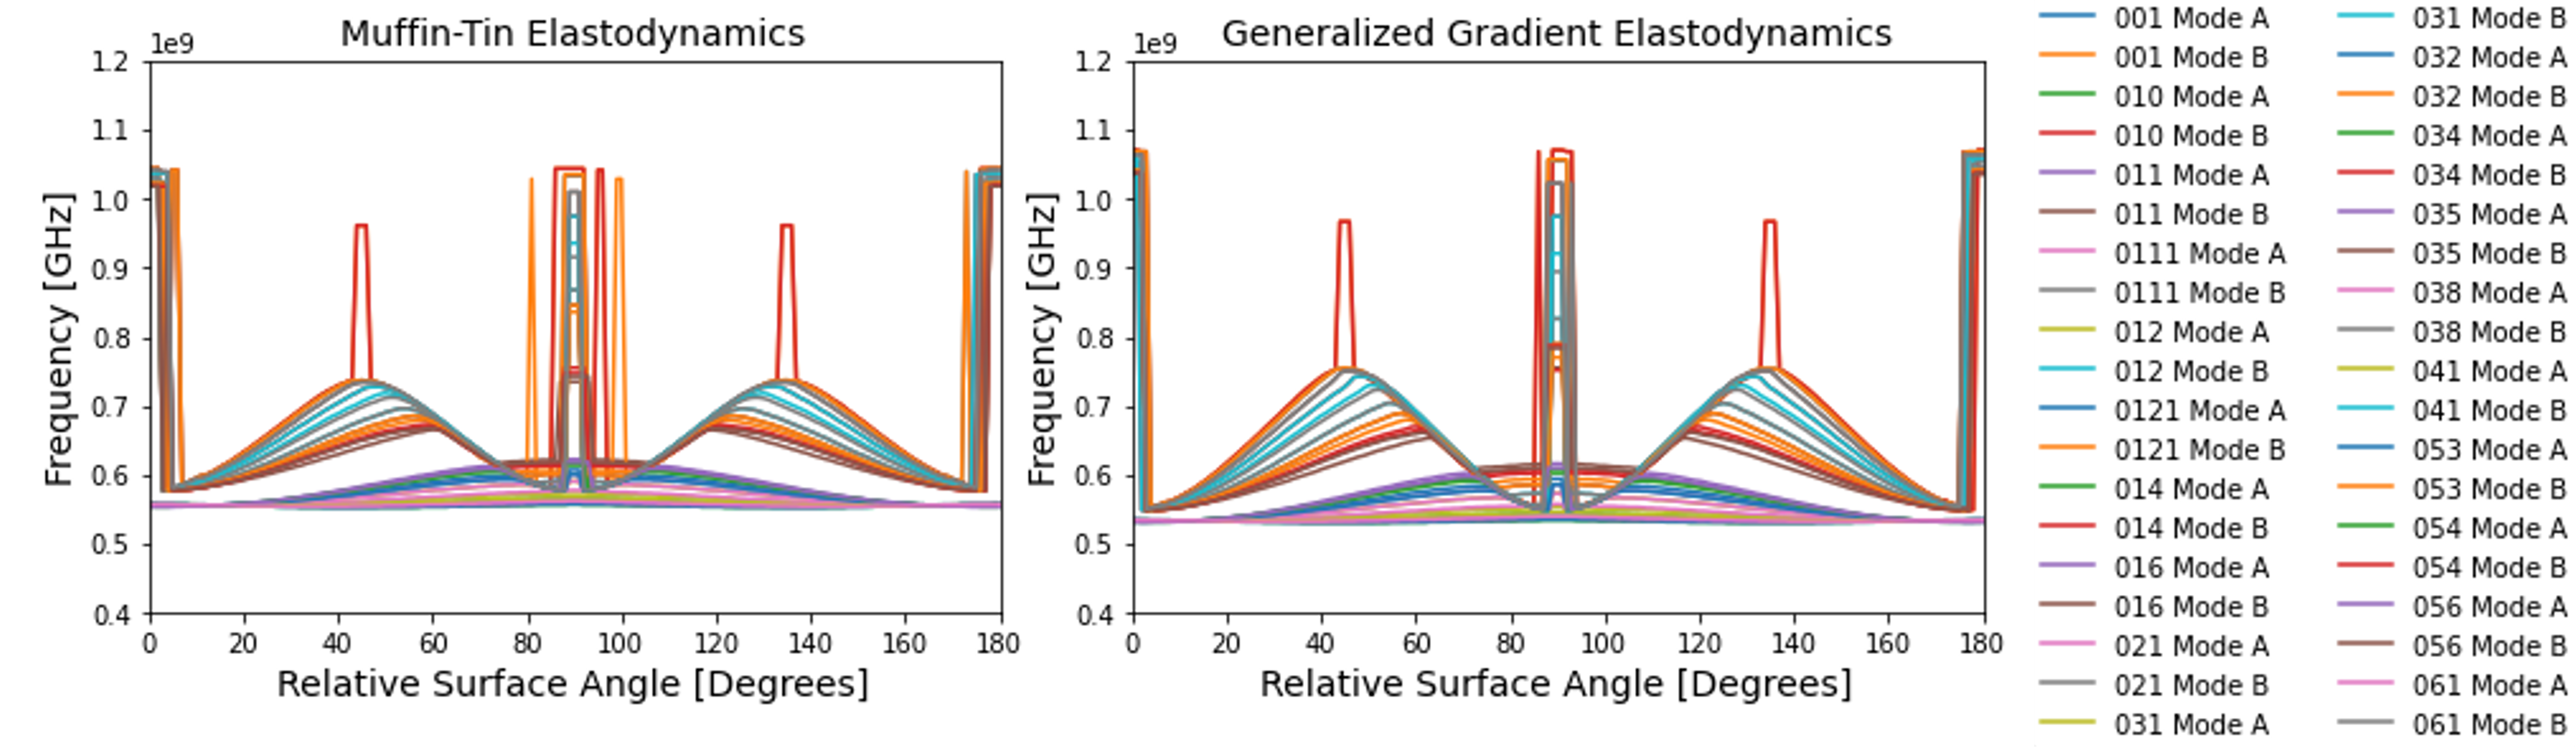
\includegraphics[width=\textwidth]{Parts/Figures/smoking-gun-v2.png}
    \caption{Quantum elastodynamic frequencies as calculated from the muffin-tin approximation and generalized gradient approximation of the ionic potential in density functional theory reveal new modes in the elastodynamically-unallowed region predicted in pristine stainless steel, and match experimentally-measured values in stainless steels that have undergone spinodal decomposition. [REF]}
    \label{fig5}
\end{sidewaysfigure}
\end{comment}
\begin{sidewaysfigure}[!ht]
    \centering
    	\begin{subfigure}{0.9\textwidth}
    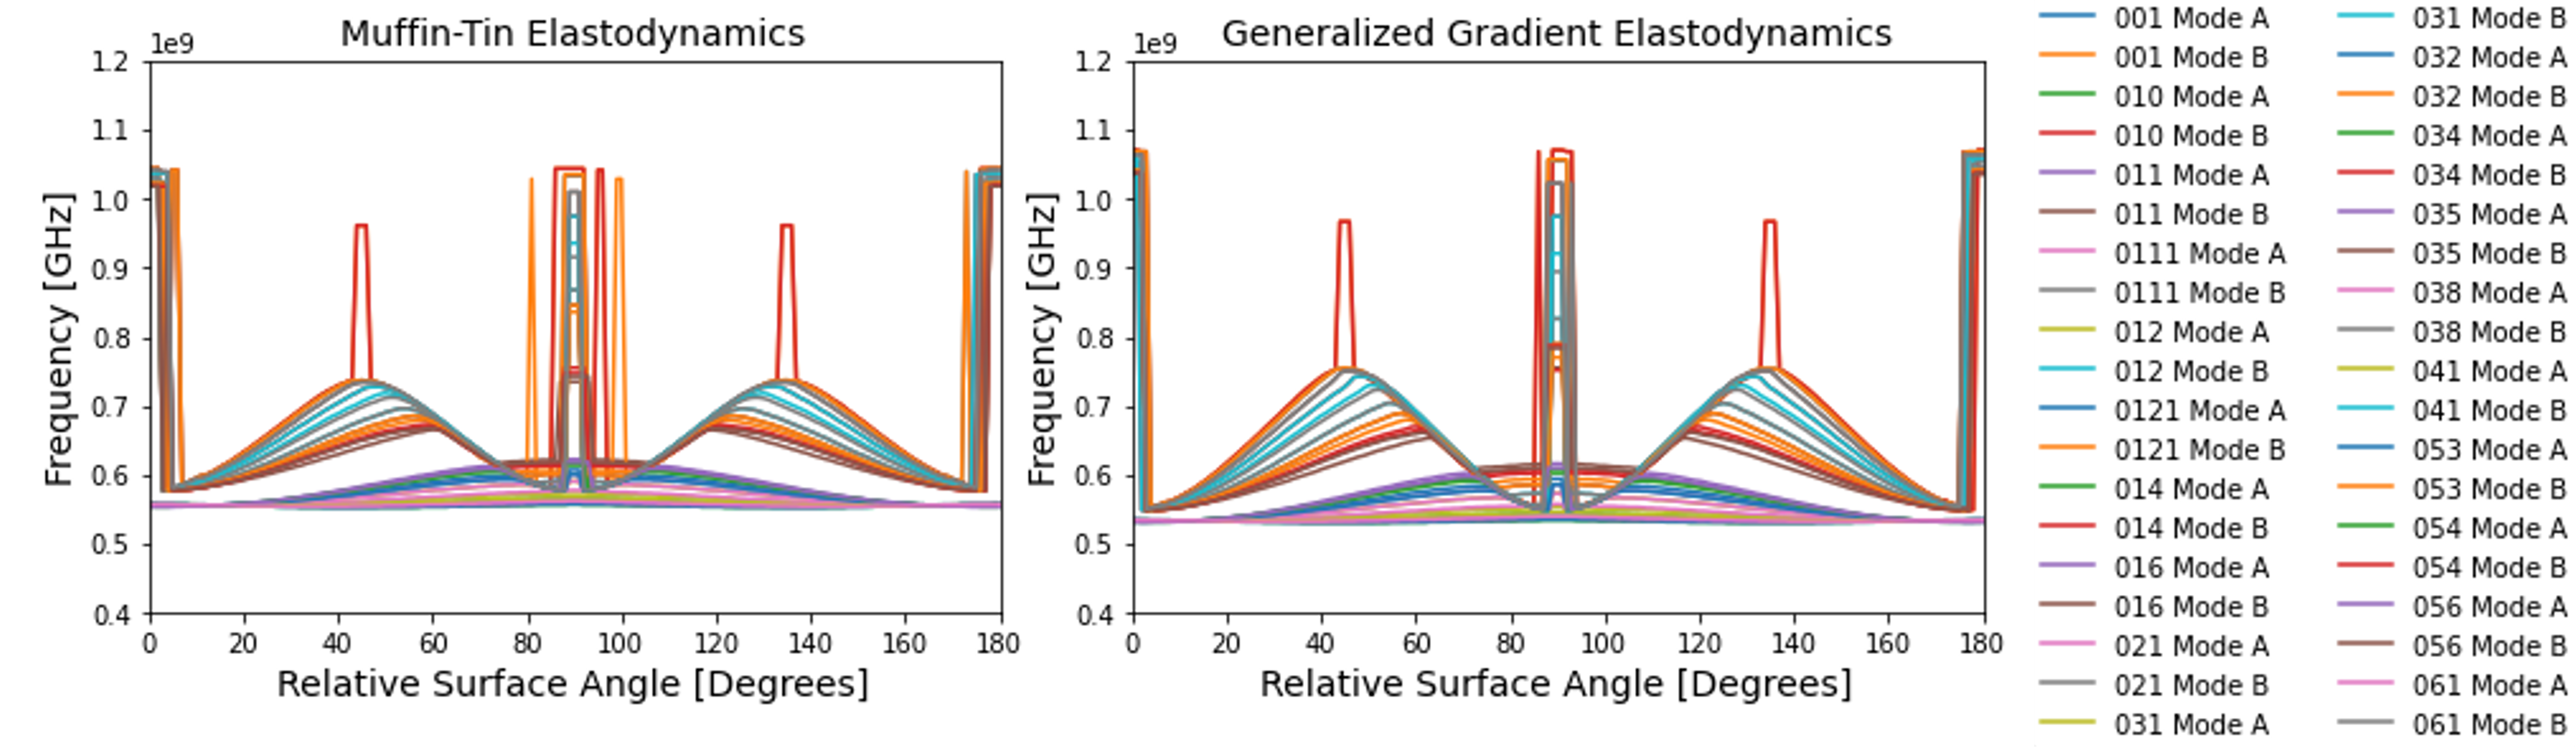
\includegraphics[width=\textwidth]{Parts/Figures/smoking-gun-v2.png}
  \caption{Predicted elastic frequencies}
         \label{fig4a}
         \end{subfigure}
        \begin{subfigure}{0.35\textwidth}
    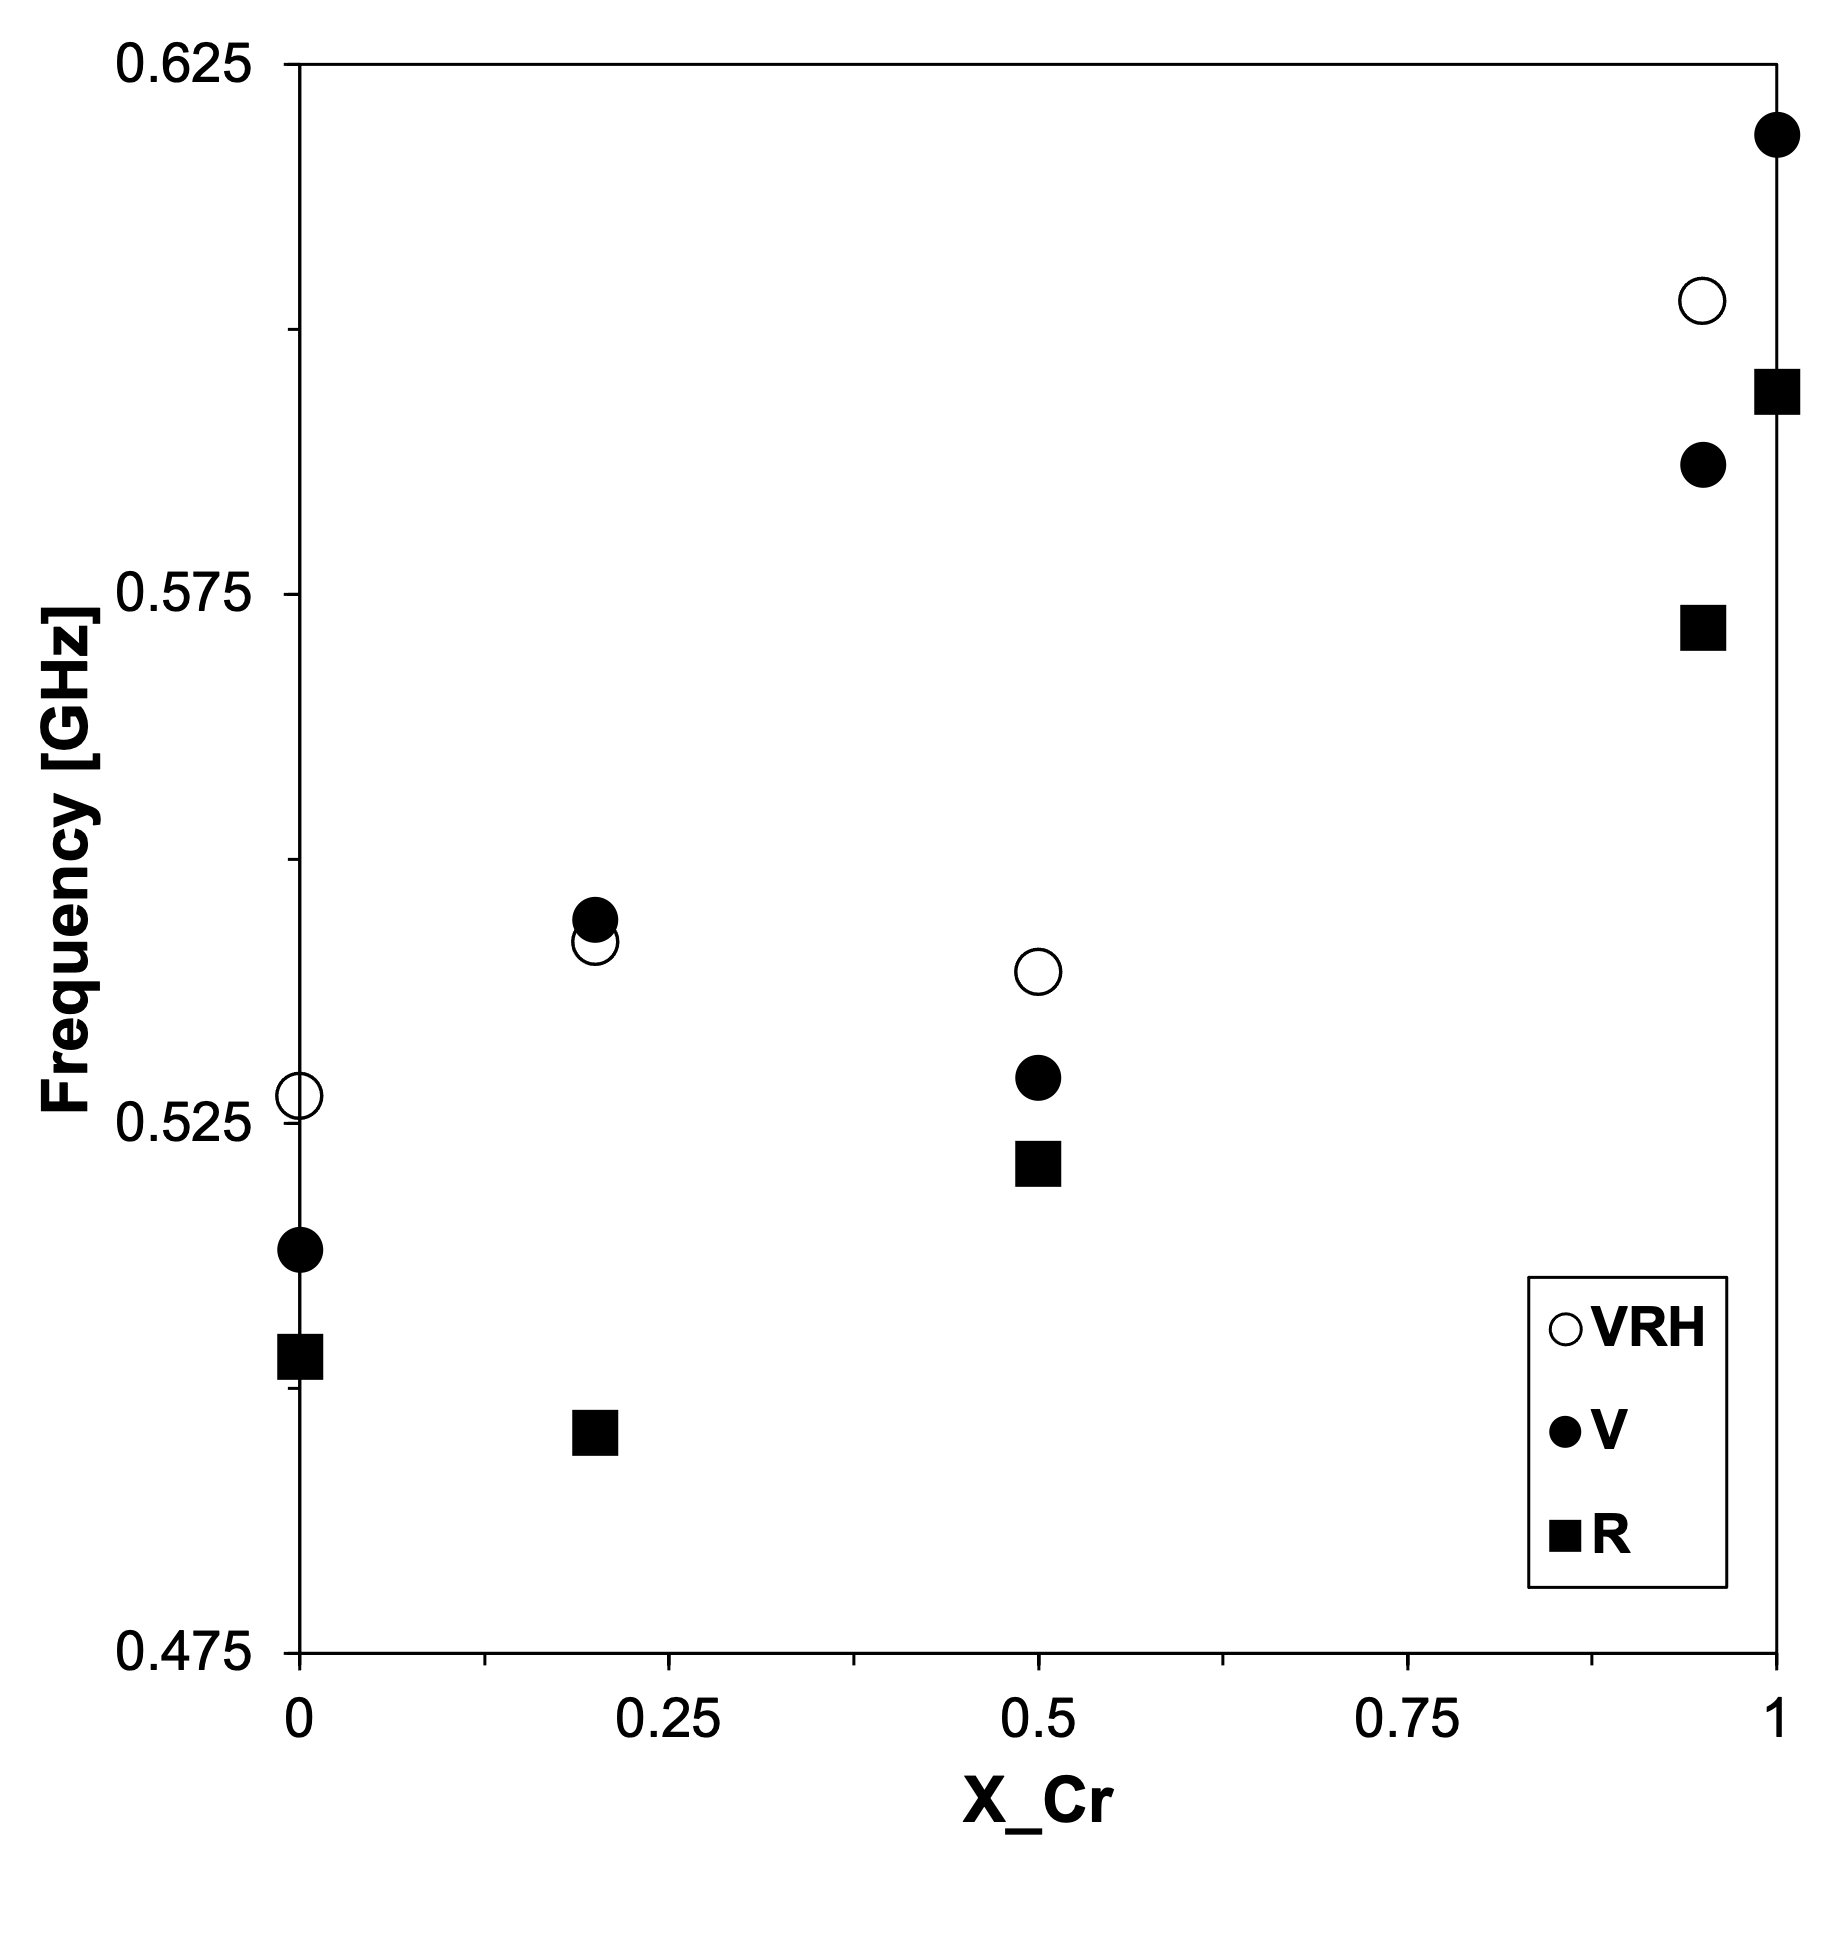
\includegraphics[width=\textwidth, left]{Parts/Figures/fvsX_v3.png}
  \caption{Calculated acoustic frequencies}
         \label{fig4b}
         \end{subfigure}
    	\begin{subfigure}{0.5\textwidth}
    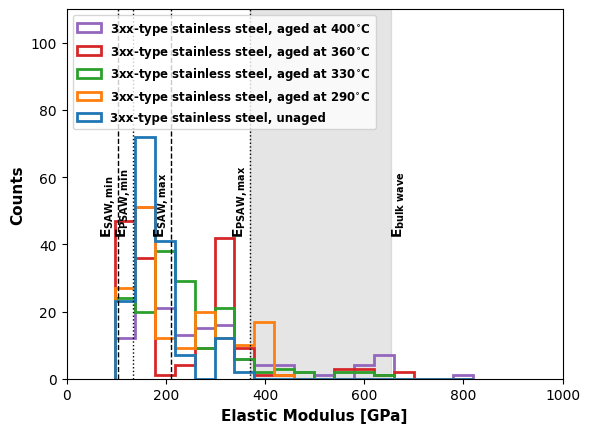
\includegraphics[width=\textwidth, right]{Parts/Figures/experimental-moduli-hist.png}
  \caption{Measured elastic moduli}
         \label{fig4c}
         \end{subfigure}
             \caption{(a) Quantum elastodynamic frequencies as calculated from the muffin-tin approximation and generalized gradient approximation of the ionic potential in density functional theory reveal new modes in the elastodynamically-unallowed region predicted in pristine stainless steel, and match experimentally-measured values in stainless steels that have undergone spinodal decomposition. [REF] (b) ... (c) ...}
    \label{fig4}
\end{sidewaysfigure}

%\begin{figure}[!ht]
%	\centering
%	\includegraphics[width=0.9\textwidth]{Parts/Figures/approximate-elastic-moduli-from-SAW-measurements.png}
%	\caption{Elastic moduli calculated from predicted SAW frequencies. Dashed red line indicates mean, and the dotted blue lines indicate range of standard deviations around the mean. Results are in agreement with calculated moduli from the elastic tensor obtained from density functional theory calculations.  }
%	\label{fig6}
%\end{figure}

\begin{comment}
    
\begin{figure}[!ht]
	\centering
	\begin{subfigure}{0.45\textwidth}
         \centering
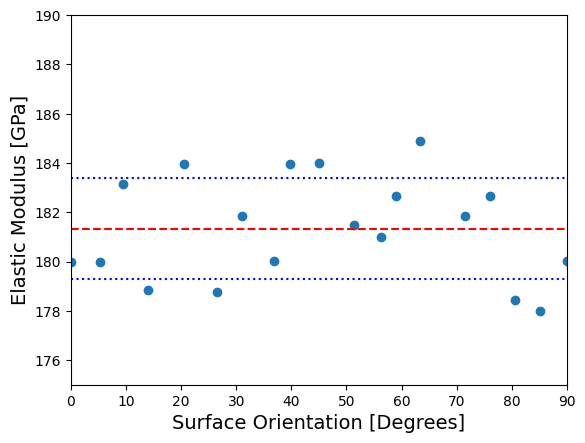
\includegraphics[width=\linewidth, left]{Parts/Figures/approximate-elastic-moduli-from-SAW-measurements-pristine.png}
         \caption{Pristine}
         \label{fig6a}
     \end{subfigure}
     \hfill
     \begin{subfigure}{0.45\textwidth}
         \centering
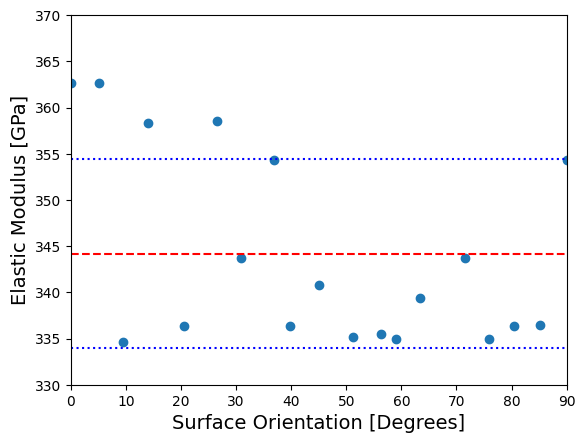
\includegraphics[width=\linewidth, right]{Parts/Figures/approximate-elastic-moduli-from-SAW-measurements-spindec.png}         \caption{Spinodal Decomposition}
         \label{fig6b}
     \end{subfigure}
	\caption{Elastic moduli calculated from predicted SAW frequencies for (a) pristine 304-type stainless steel and (b) spinodally decomposed 304-type stainless steel. Dashed red lines indicates mean, and the dotted blue lines indicate range of standard deviations around the mean. Results in (b) are in agreement with calculated moduli from the elastic tensor obtained from density functional theory calculations in Fig. \ref{fig3a}, and comparison of (a) and (b) confirm stiffening induced by spinodal decomposition as observed in [REF].  }
	\label{fig6}
\end{figure}


\begin{figure}[!ht]
	\centering
	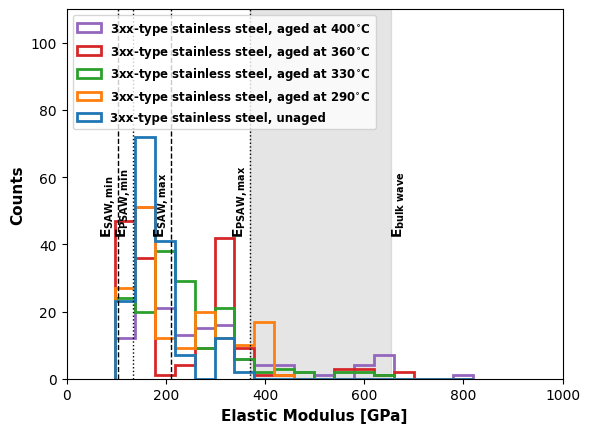
\includegraphics[width=0.9\textwidth]{Parts/Figures/experimental-moduli-hist.png}
	\caption{Elastic moduli calculated from measured SAW frequencies for unaged and thermally aged 304 and 316-type stainless steel in [REF]. Dashed lines indicates type of wave speed used to calculate elastic moduli in those regions. Shaded region corresponds to elastodynamically-unallowed range of frequencies observed in [REF] attributed to thermally-induced stiffening of $\delta$-ferrite as a result of spinodal decomposition. Aged specimens consistently show stiffening with higher elastic moduli than unaged, as shown in the tails of the distributions of elastic moduli calculated for aged steels. }
	\label{fig7}
\end{figure}

\begin{figure}[!ht]
	\centering
	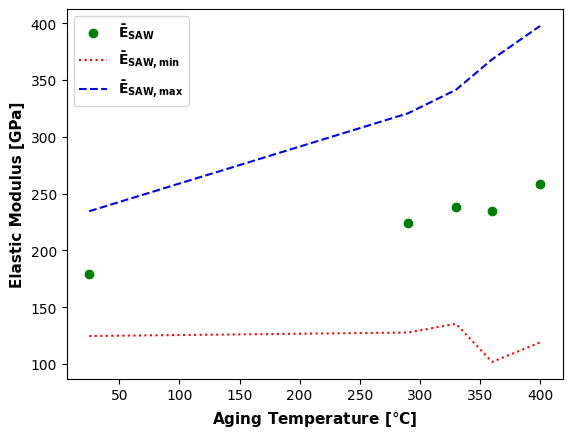
\includegraphics[width=0.9\textwidth]{Parts/Figures/experimental-moduli-trend.png}
	\caption{Elastic moduli as a function of aging temperature calculated from measured SAW frequencies for unaged and thermally aged 304 and 316-type stainless steel in [REF]. Elastic moduli for aged samples calculated from experimental SAW speeds are consistent with elastic moduli calculated from simplied density functional theory simulations of these alloys in Fig. \ref{fig3a}. As observed in [REF], the large error bounds in these values are due to the likelihood of a surface acoustic wave to probe both $\delta$-ferrite and $\gamma$-austenite, where $\delta$-ferrite grains are stiffened by spinodal decomposition and $\gamma$-austenite grains remain mechanically intact. However, the experimental and theoretical values consistently fall within the upper bounds on these calculations, consistent with density functional theory calculations in Fig. \ref{fig3a} combined with elastodynamic simulations in Fig. \ref{fig5}. }
	\label{fig8}
\end{figure}
\end{comment}


\begin{comment}
    
\begin{figure}[!ht]
	\centering
	\begin{subfigure}{0.45\textwidth}
         \centering
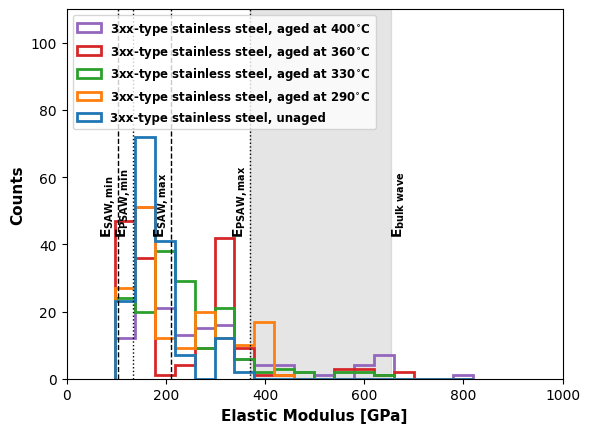
\includegraphics[width=\linewidth, left]{Parts/Figures/experimental-moduli-hist.png}
         \caption{Histogram}
         \label{fig6a}
     \end{subfigure}
     \hfill
     \begin{subfigure}{0.45\textwidth}
         \centering
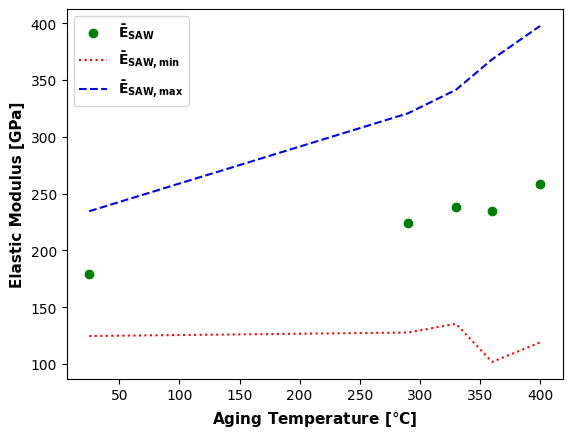
\includegraphics[width=\linewidth, right]{Parts/Figures/experimental-moduli-trend.png}         
\caption{Aging Trend}
         \label{fig6b}
     \end{subfigure}
	\caption{Elastic moduli calculated from measured SAW frequencies for unaged and thermally aged 304 and 316-type stainless steel. Dashed red lines indicates mean, and the dotted blue lines indicate range of standard deviations around the mean. Results in (b) are in agreement with calculated moduli from the elastic tensor obtained from density functional theory calculations, and comparison of (a) and (b) confirm stiffening induced by spinodal decomposition.  }
	\label{fig6}
\end{figure}
\end{comment}

\begin{comment}
    
\begin{sidewaysfigure}
	\centering
	\begin{subfigure}{0.3\textwidth}
         \centering
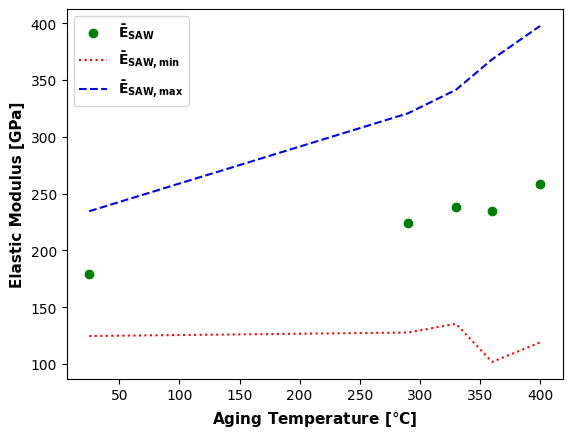
\includegraphics[width=\linewidth, left]{Parts/Figures/experimental-moduli-trend.png}
         \caption{Experimental elastic moduli of aged steels}
         \label{fig4a}
     \end{subfigure}
     \hfill
     \begin{subfigure}{0.3\textwidth}
         \centering
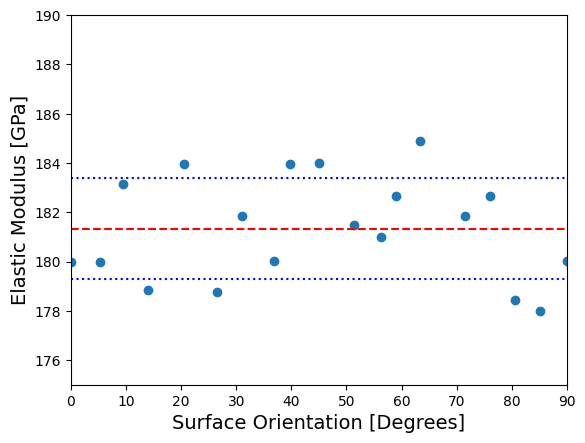
\includegraphics[width=\linewidth, left]{Parts/Figures/approximate-elastic-moduli-from-SAW-measurements-pristine.png}
         \caption{Theoretical elastic moduli of pristine steels}
         \label{fig6a}
     \end{subfigure}
     \hfill
     \begin{subfigure}{0.3\textwidth}
         \centering
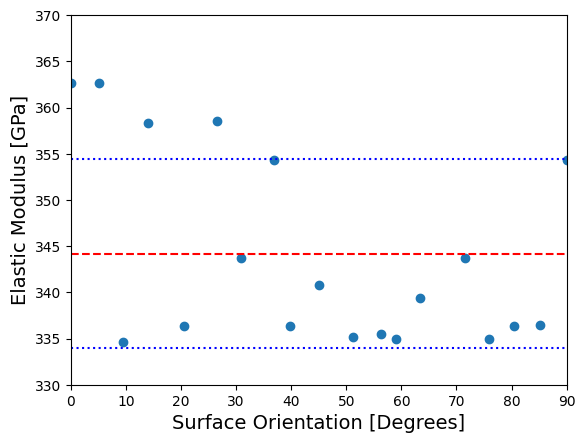
\includegraphics[width=\linewidth, right]{Parts/Figures/approximate-elastic-moduli-from-SAW-measurements-spindec.png}         \caption{Theoretical elastic moduli of spinodally decomposed steels}
         \label{fig6b}
     \end{subfigure}
     \hfill
    \begin{subfigure}{0.3\textwidth}
         \centering
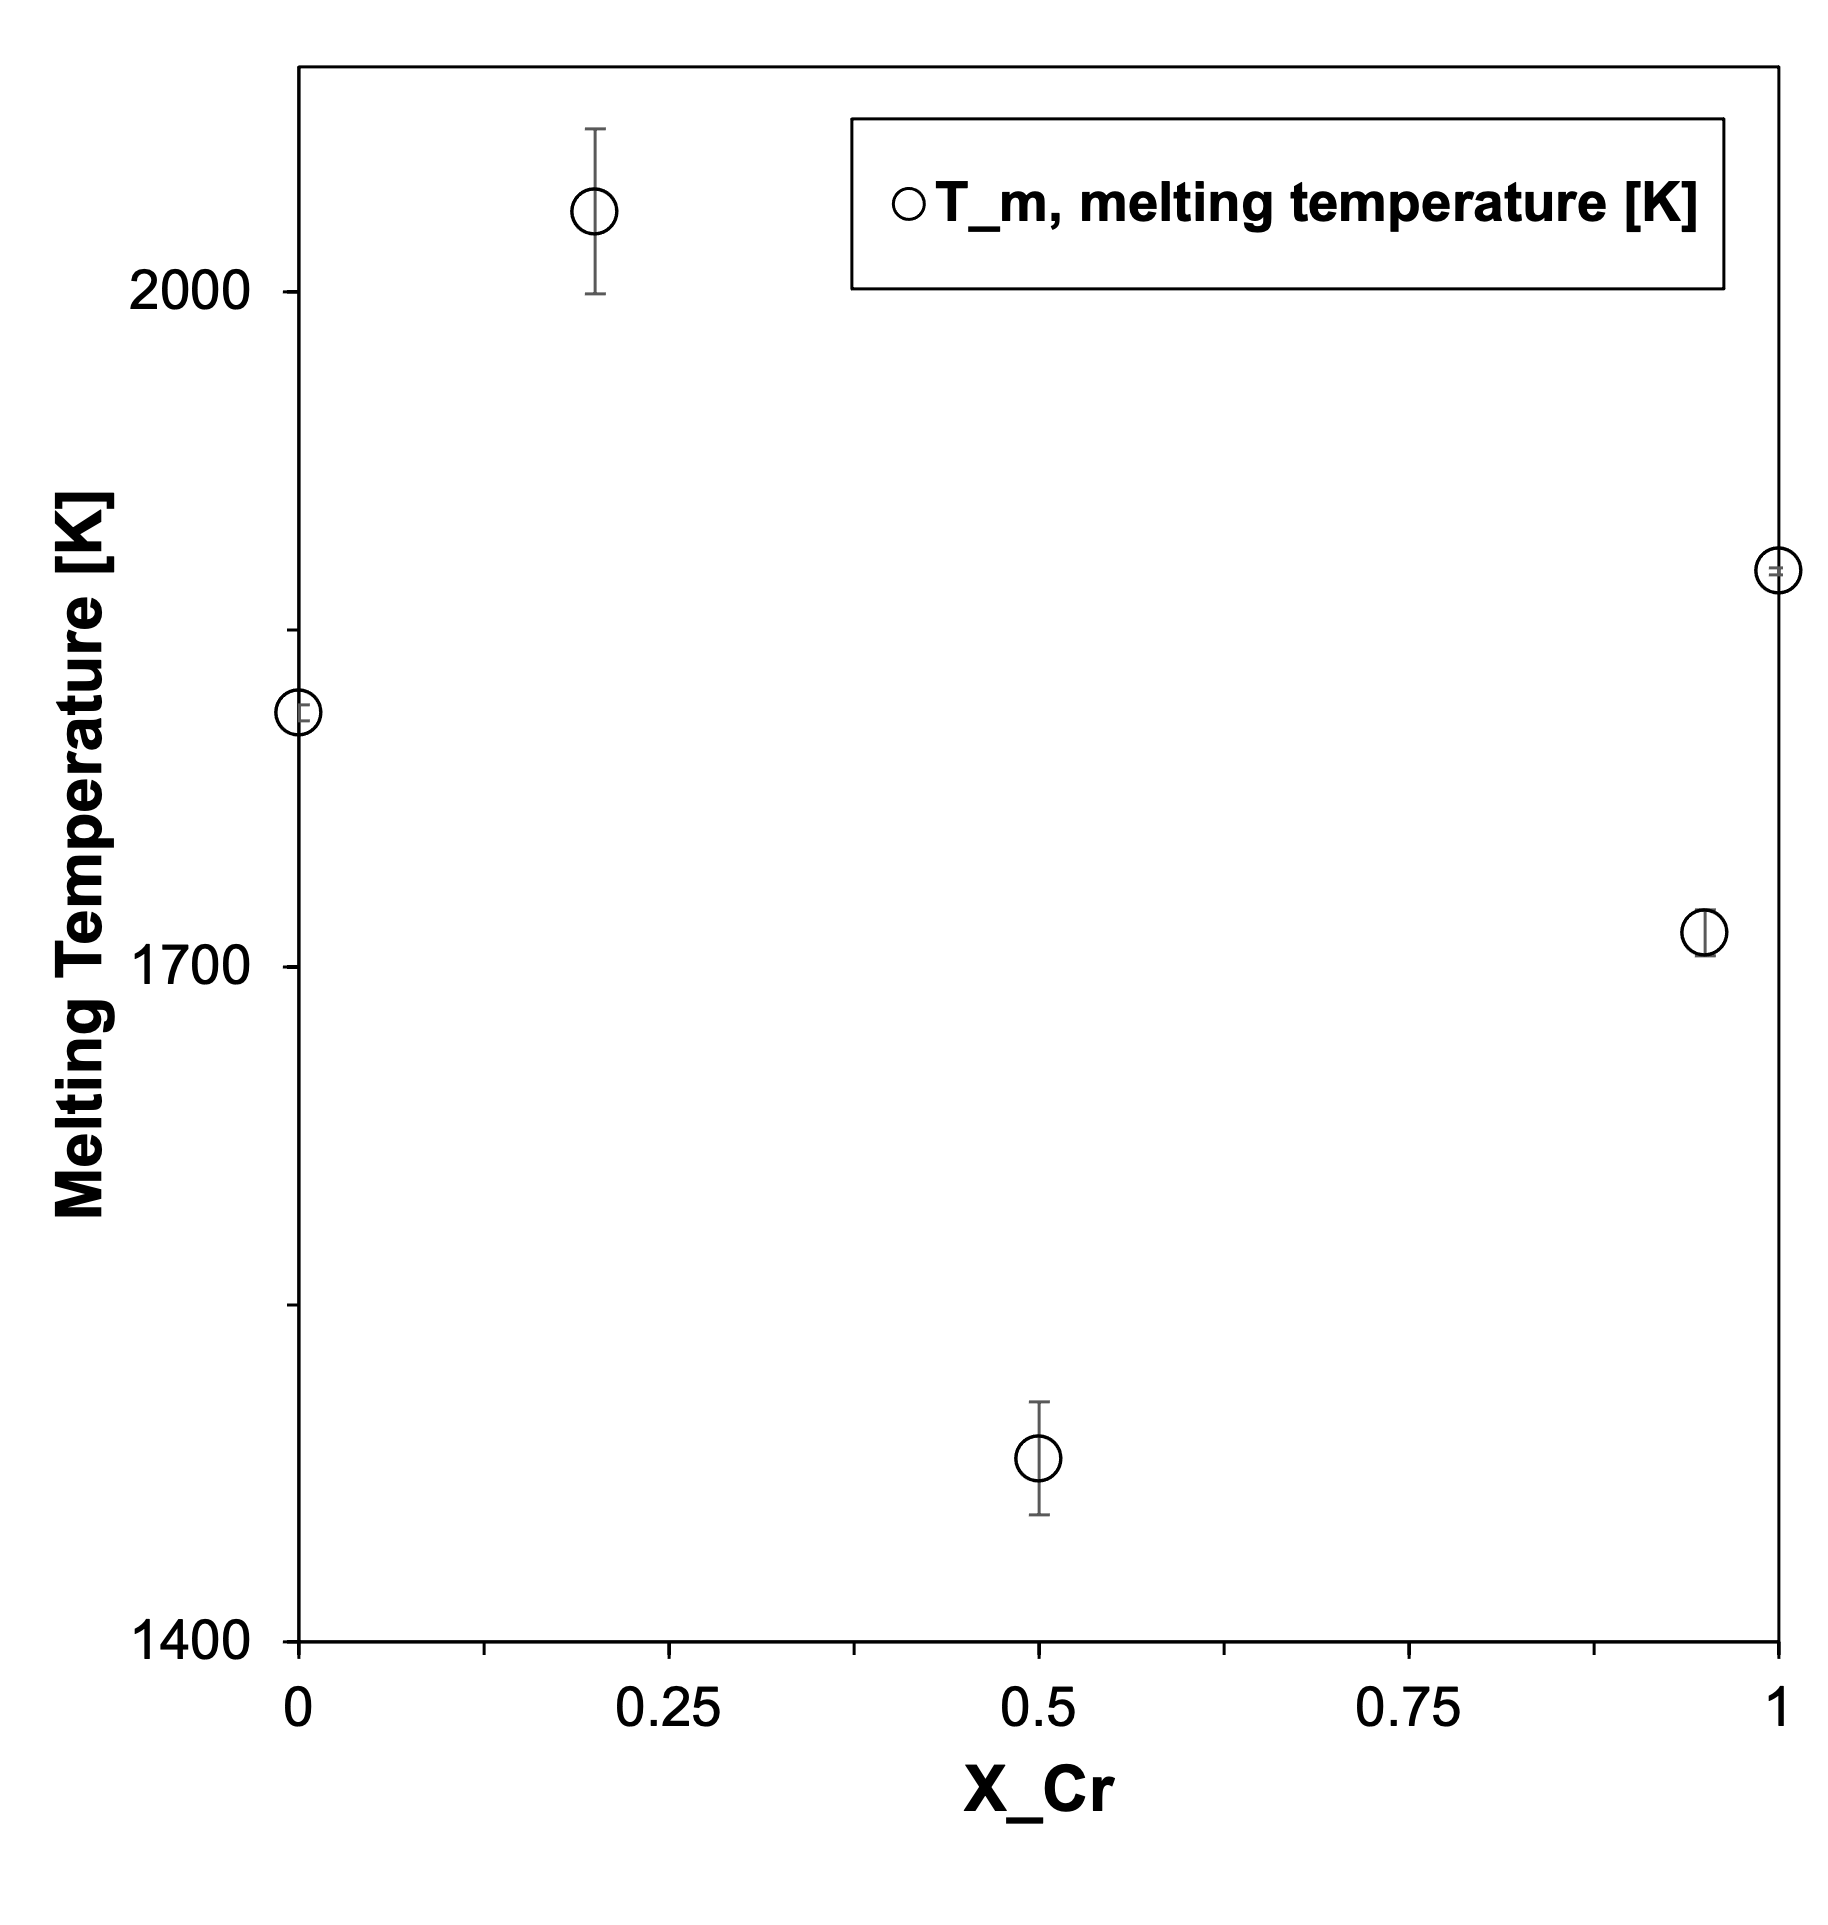
\includegraphics[width=\linewidth, left]{Parts/Figures/TMvsX_v2.png}
         \caption{$T_M$, melting temperature}
         \label{fig1a}
     \end{subfigure}
     \hfill
     \begin{subfigure}{0.3\textwidth}
         \centering
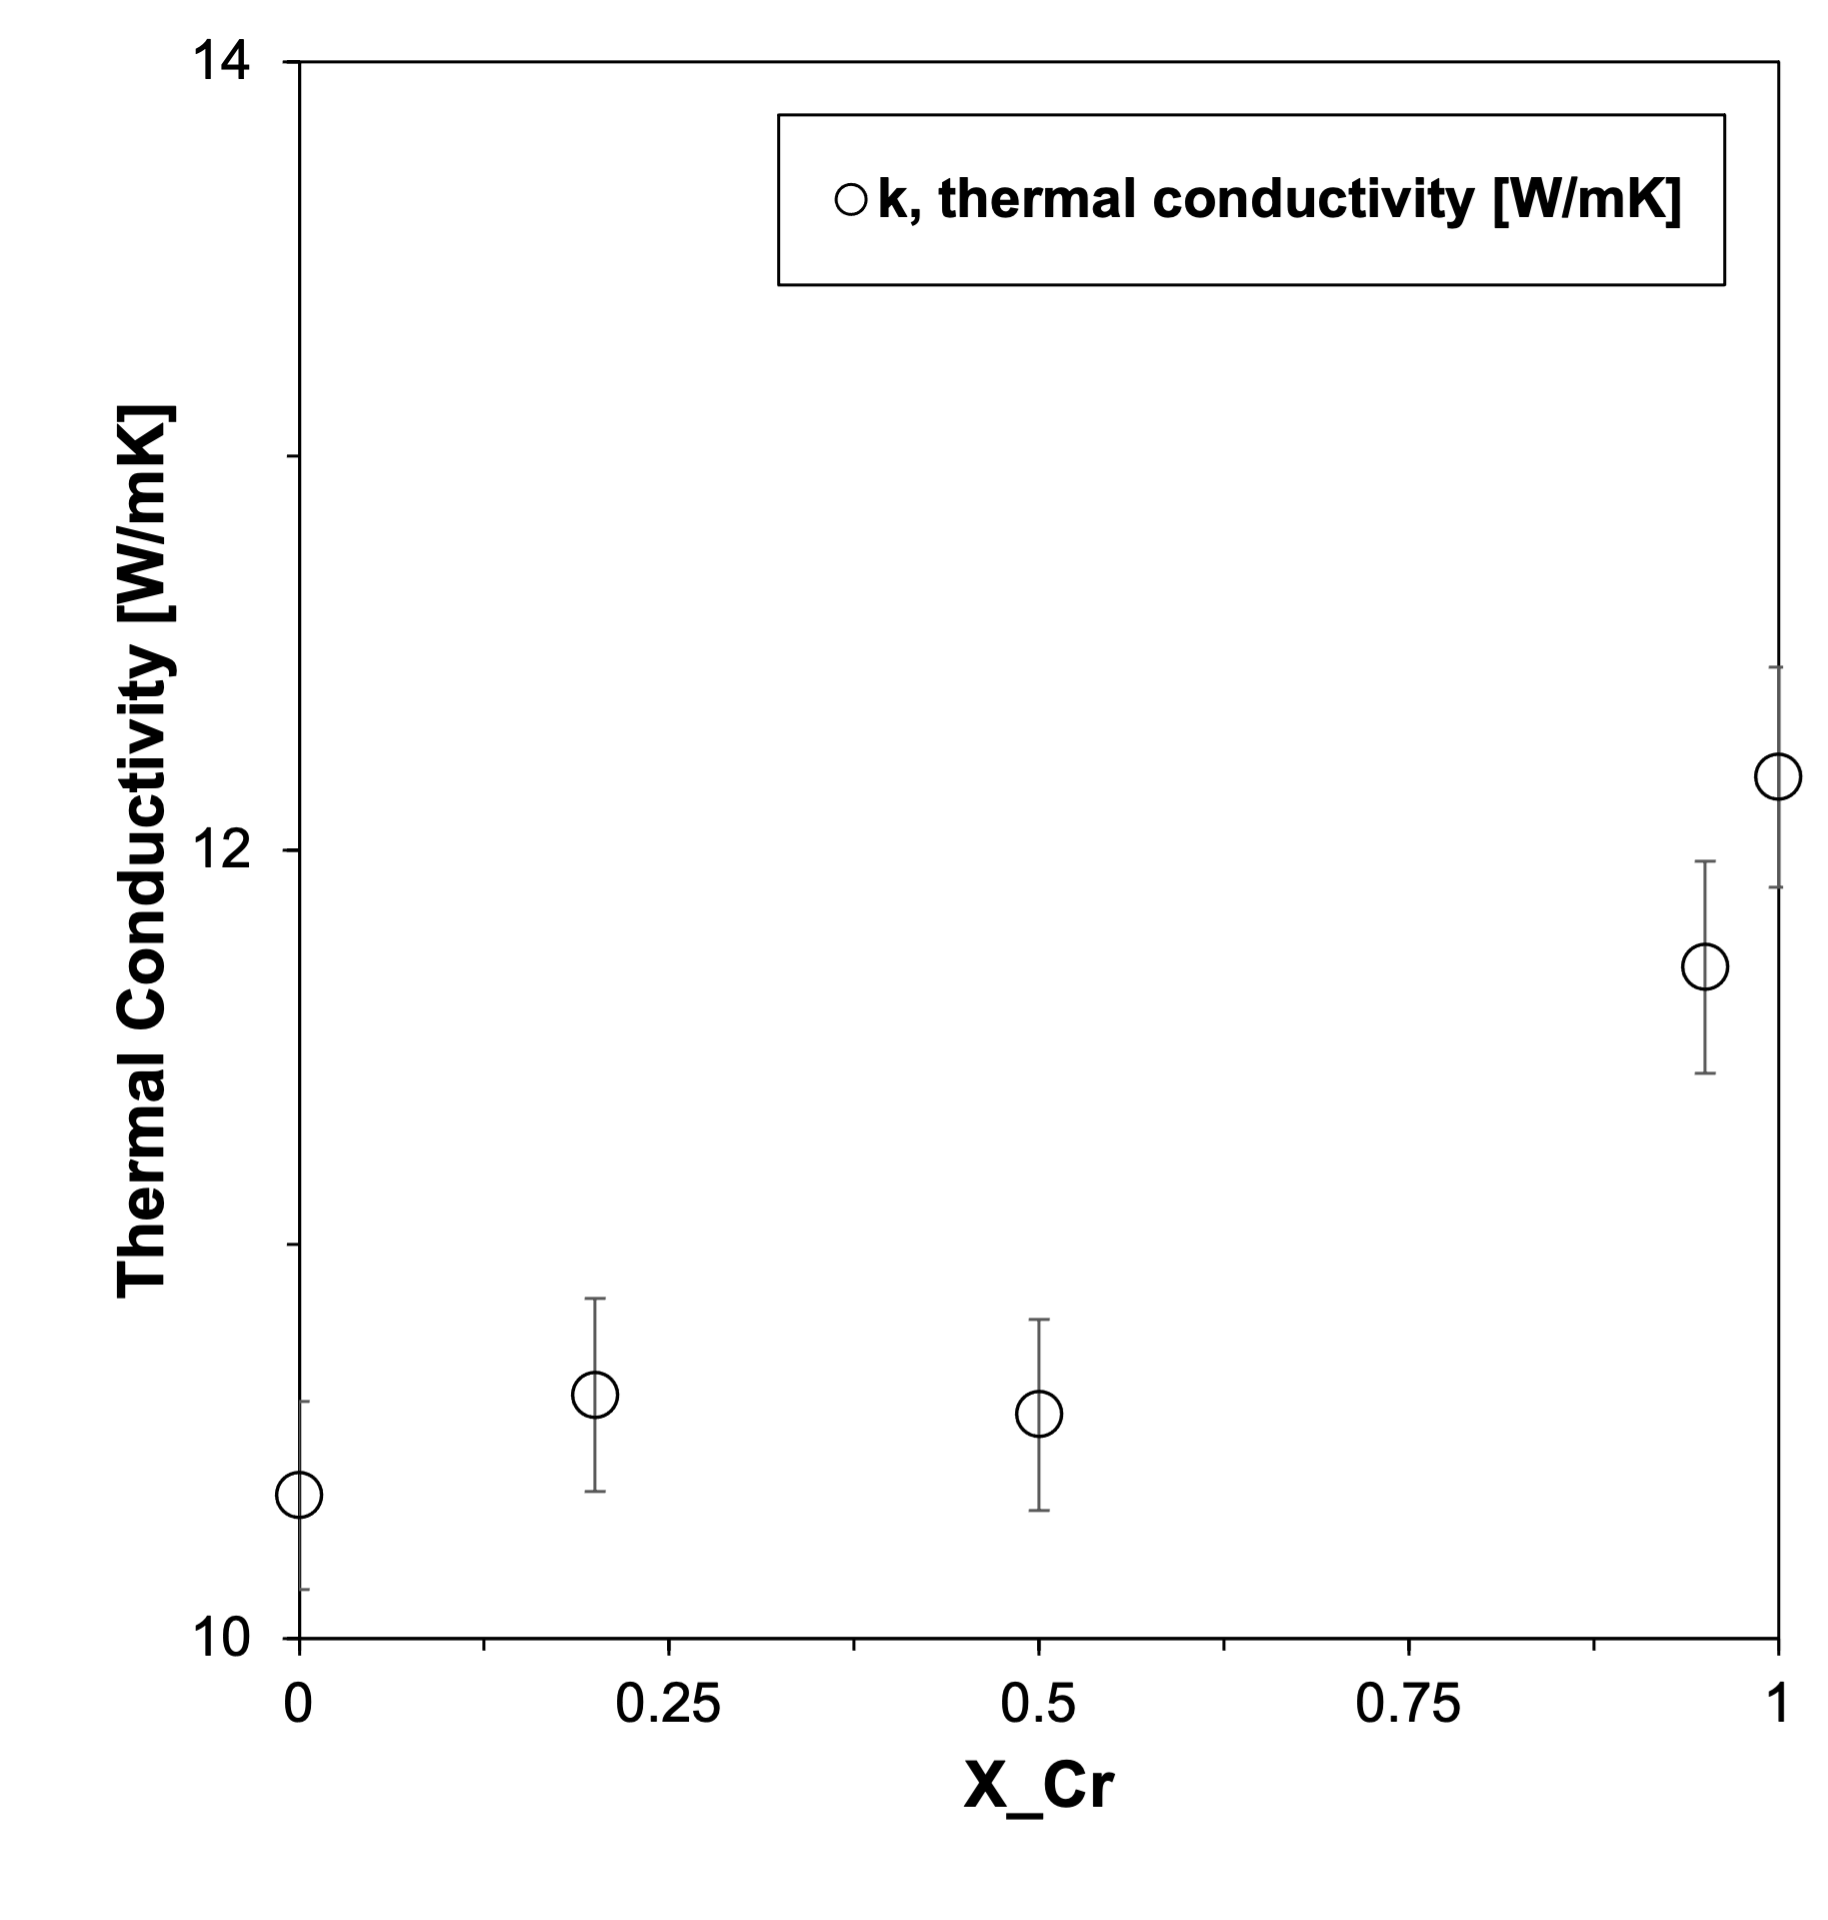
\includegraphics[width=\linewidth, right]{Parts/Figures/KvsX_v2.png}         \caption{$\kappa$, thermal conductivity}
         \label{fig4b}
     \end{subfigure}
          \hfill
     	\begin{subfigure}{0.3\textwidth}
         \centering
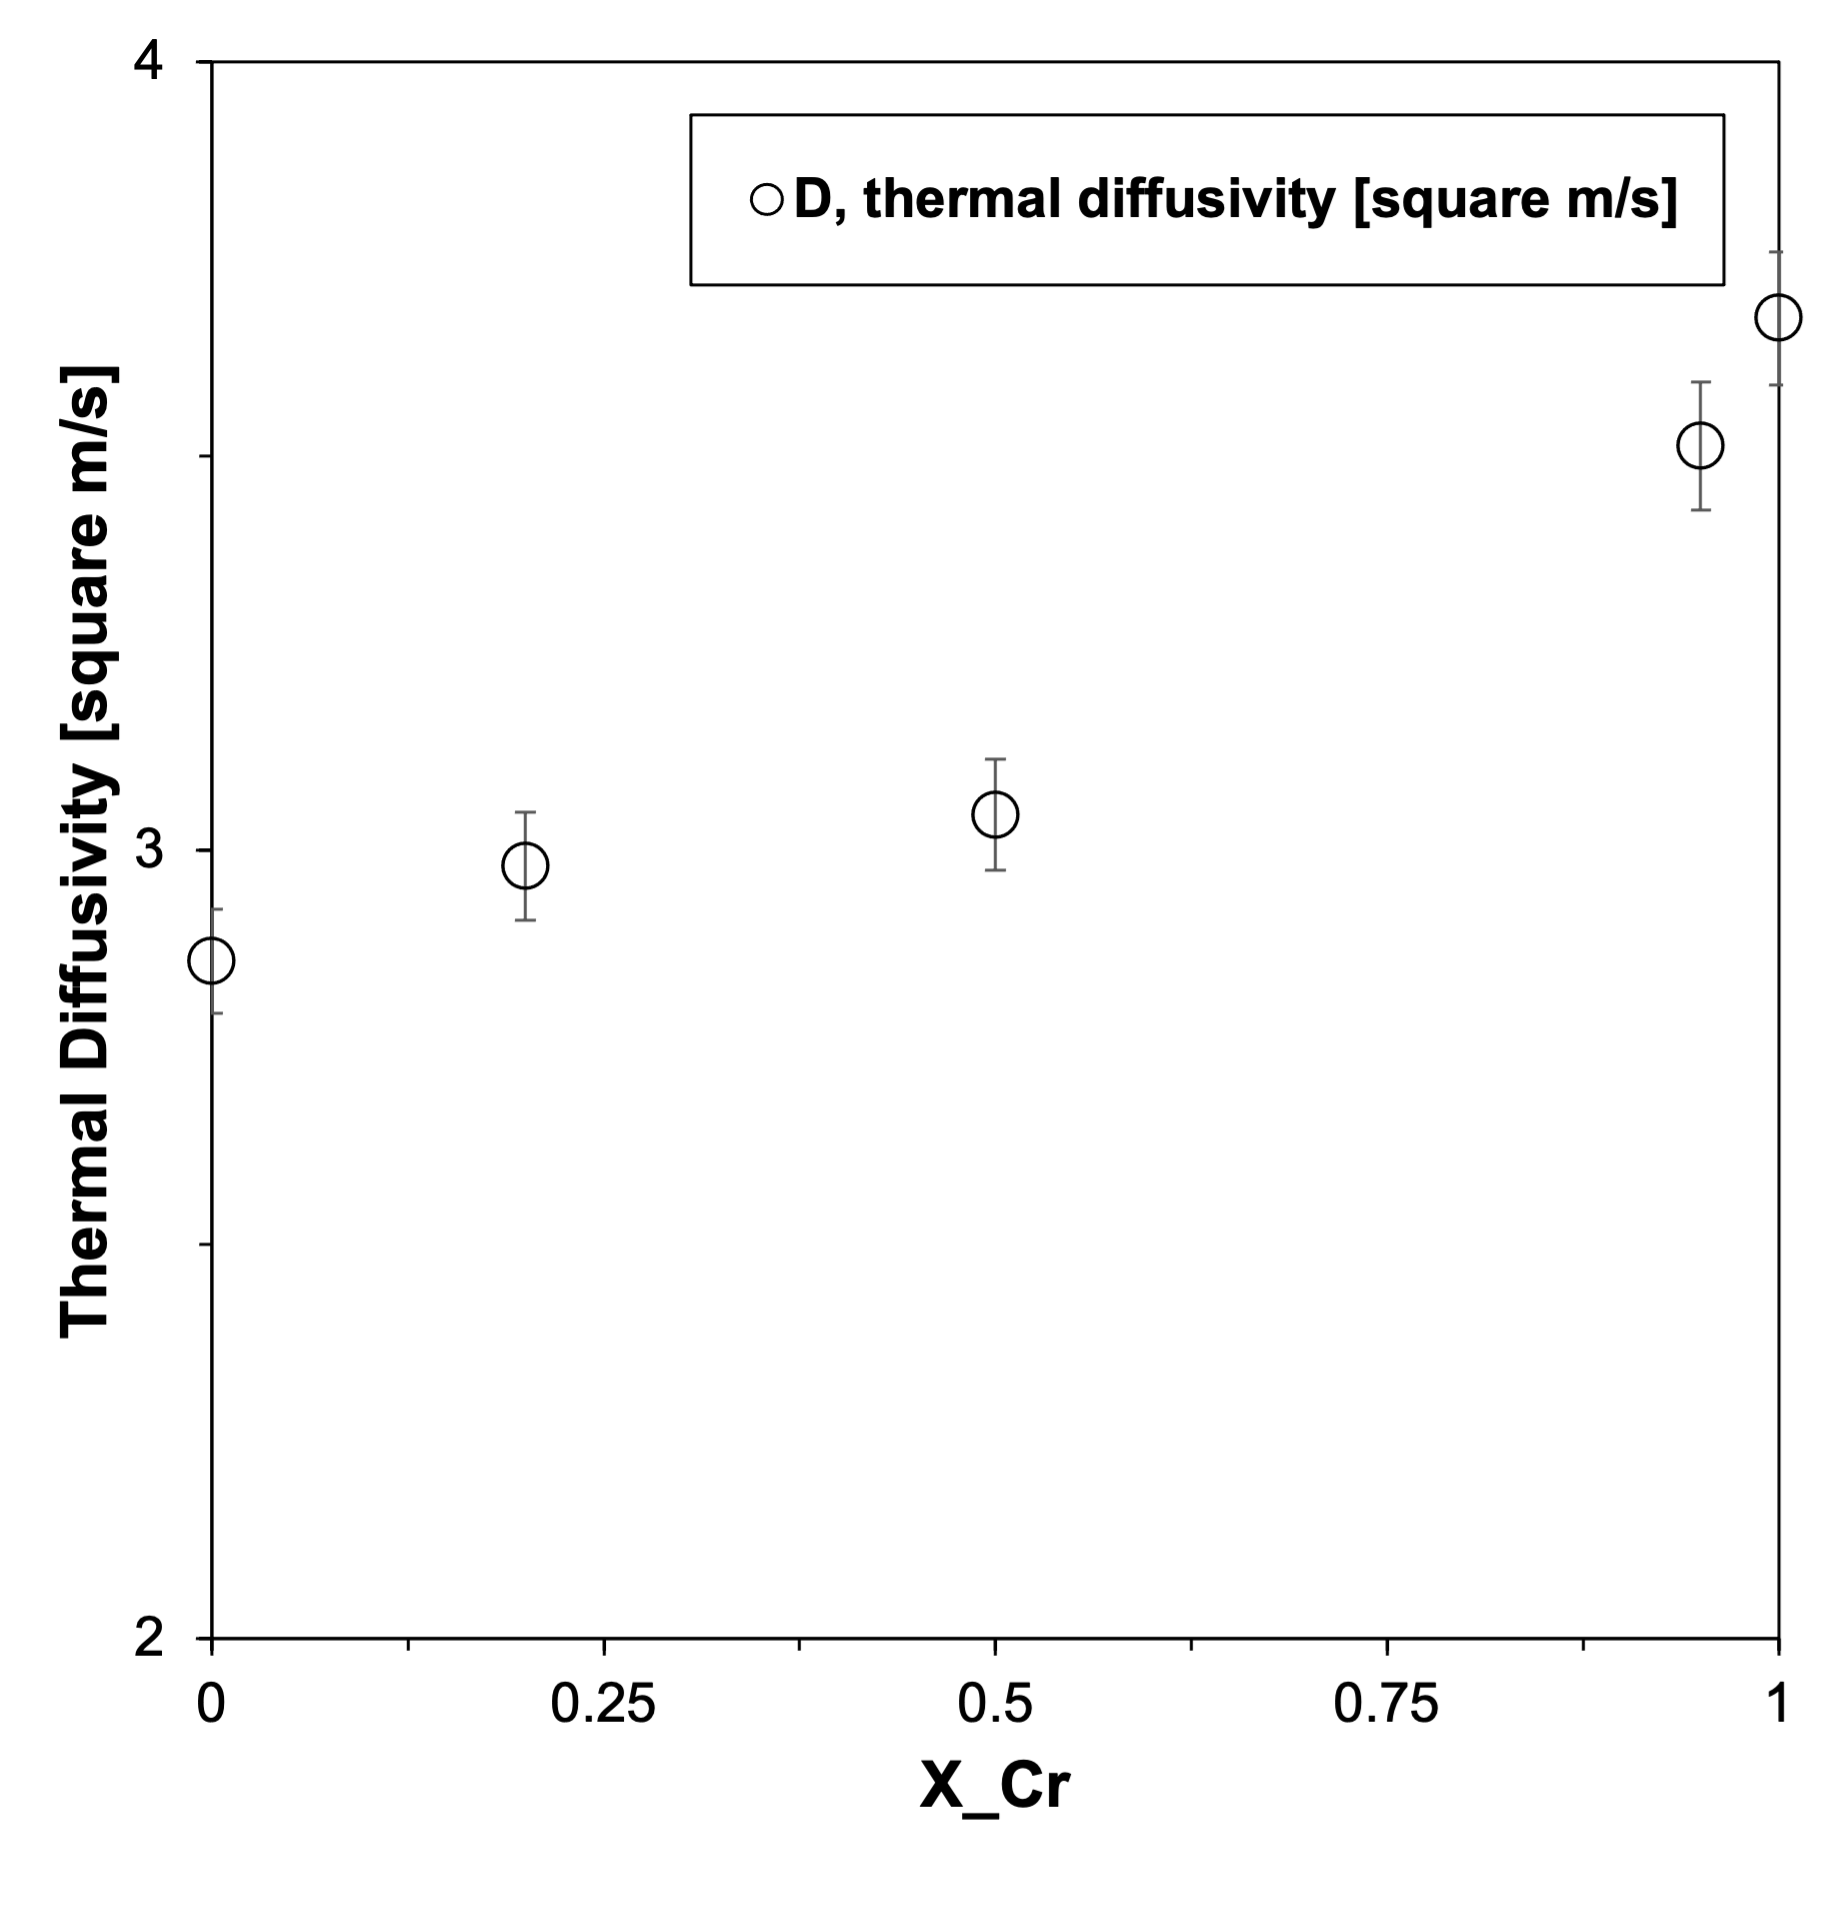
\includegraphics[width=\linewidth, left]{Parts/Figures/DvsX_v2.png}
         \caption{$D$, thermal diffusivity}
         \label{fig4a}
     \end{subfigure}
	\caption{(a) Elastic moduli as a function of aging temperature calculated from measured SAW frequencies for unaged and thermally aged 304 and 316-type stainless steel in [REF]. Elastic moduli for aged samples calculated from experimental SAW speeds are consistent with elastic moduli calculated from simplied density functional theory simulations of these alloys in Fig. \ref{fig3a}. As observed in [REF], the large error bounds in these values are due to the likelihood of a surface acoustic wave to probe both $\delta$-ferrite and $\gamma$-austenite, where $\delta$-ferrite grains are stiffened by spinodal decomposition and $\gamma$-austenite grains remain mechanically intact. However, the experimental and theoretical values consistently fall within the upper bounds on these calculations, consistent with density functional theory calculations in Fig. \ref{fig3a} combined with elastodynamic simulations in Fig. \ref{fig4a}. (b) ... (c) ...}
	\label{fig4}
\end{sidewaysfigure}
\end{comment}

\begin{sidewaysfigure}[!ht]
	\centering
	\begin{subfigure}{0.3\textwidth}
         \centering
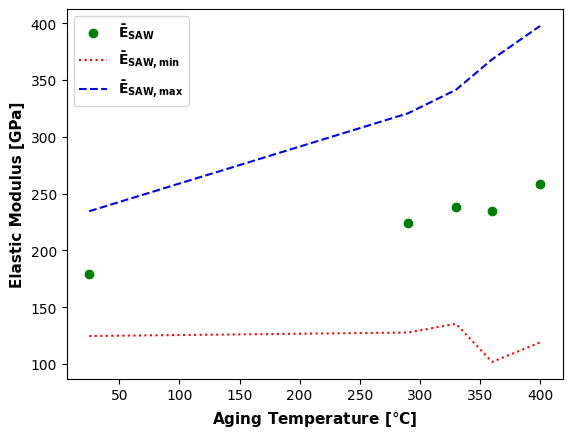
\includegraphics[width=\linewidth, left]{Parts/Figures/experimental-moduli-trend.png}
         \caption{Experimental elastic moduli of aged steels}
         \label{fig5a}
     \end{subfigure}
     \hfill
     \begin{subfigure}{0.3\textwidth}
         \centering
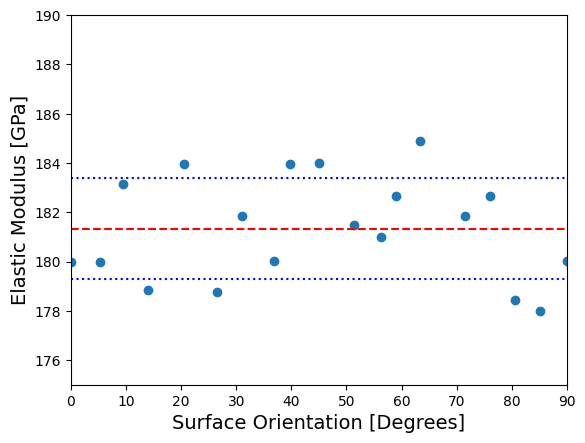
\includegraphics[width=\linewidth, left]{Parts/Figures/approximate-elastic-moduli-from-SAW-measurements-pristine.png}
         \caption{Theoretical elastic moduli of pristine steels}
         \label{fig5b}
     \end{subfigure}
     \hfill
     \begin{subfigure}{0.3\textwidth}
         \centering
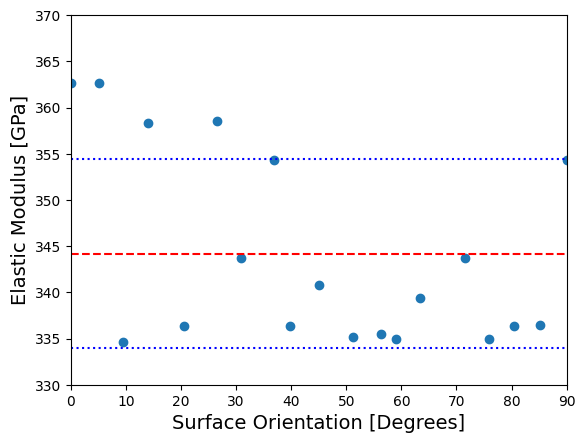
\includegraphics[width=\linewidth, right]{Parts/Figures/approximate-elastic-moduli-from-SAW-measurements-spindec.png}         \caption{Theoretical elastic moduli of spinodally decomposed steels}
         \label{fig5c}
     \end{subfigure}
     \hfill
     \begin{subfigure}{0.3\textwidth}
         \centering
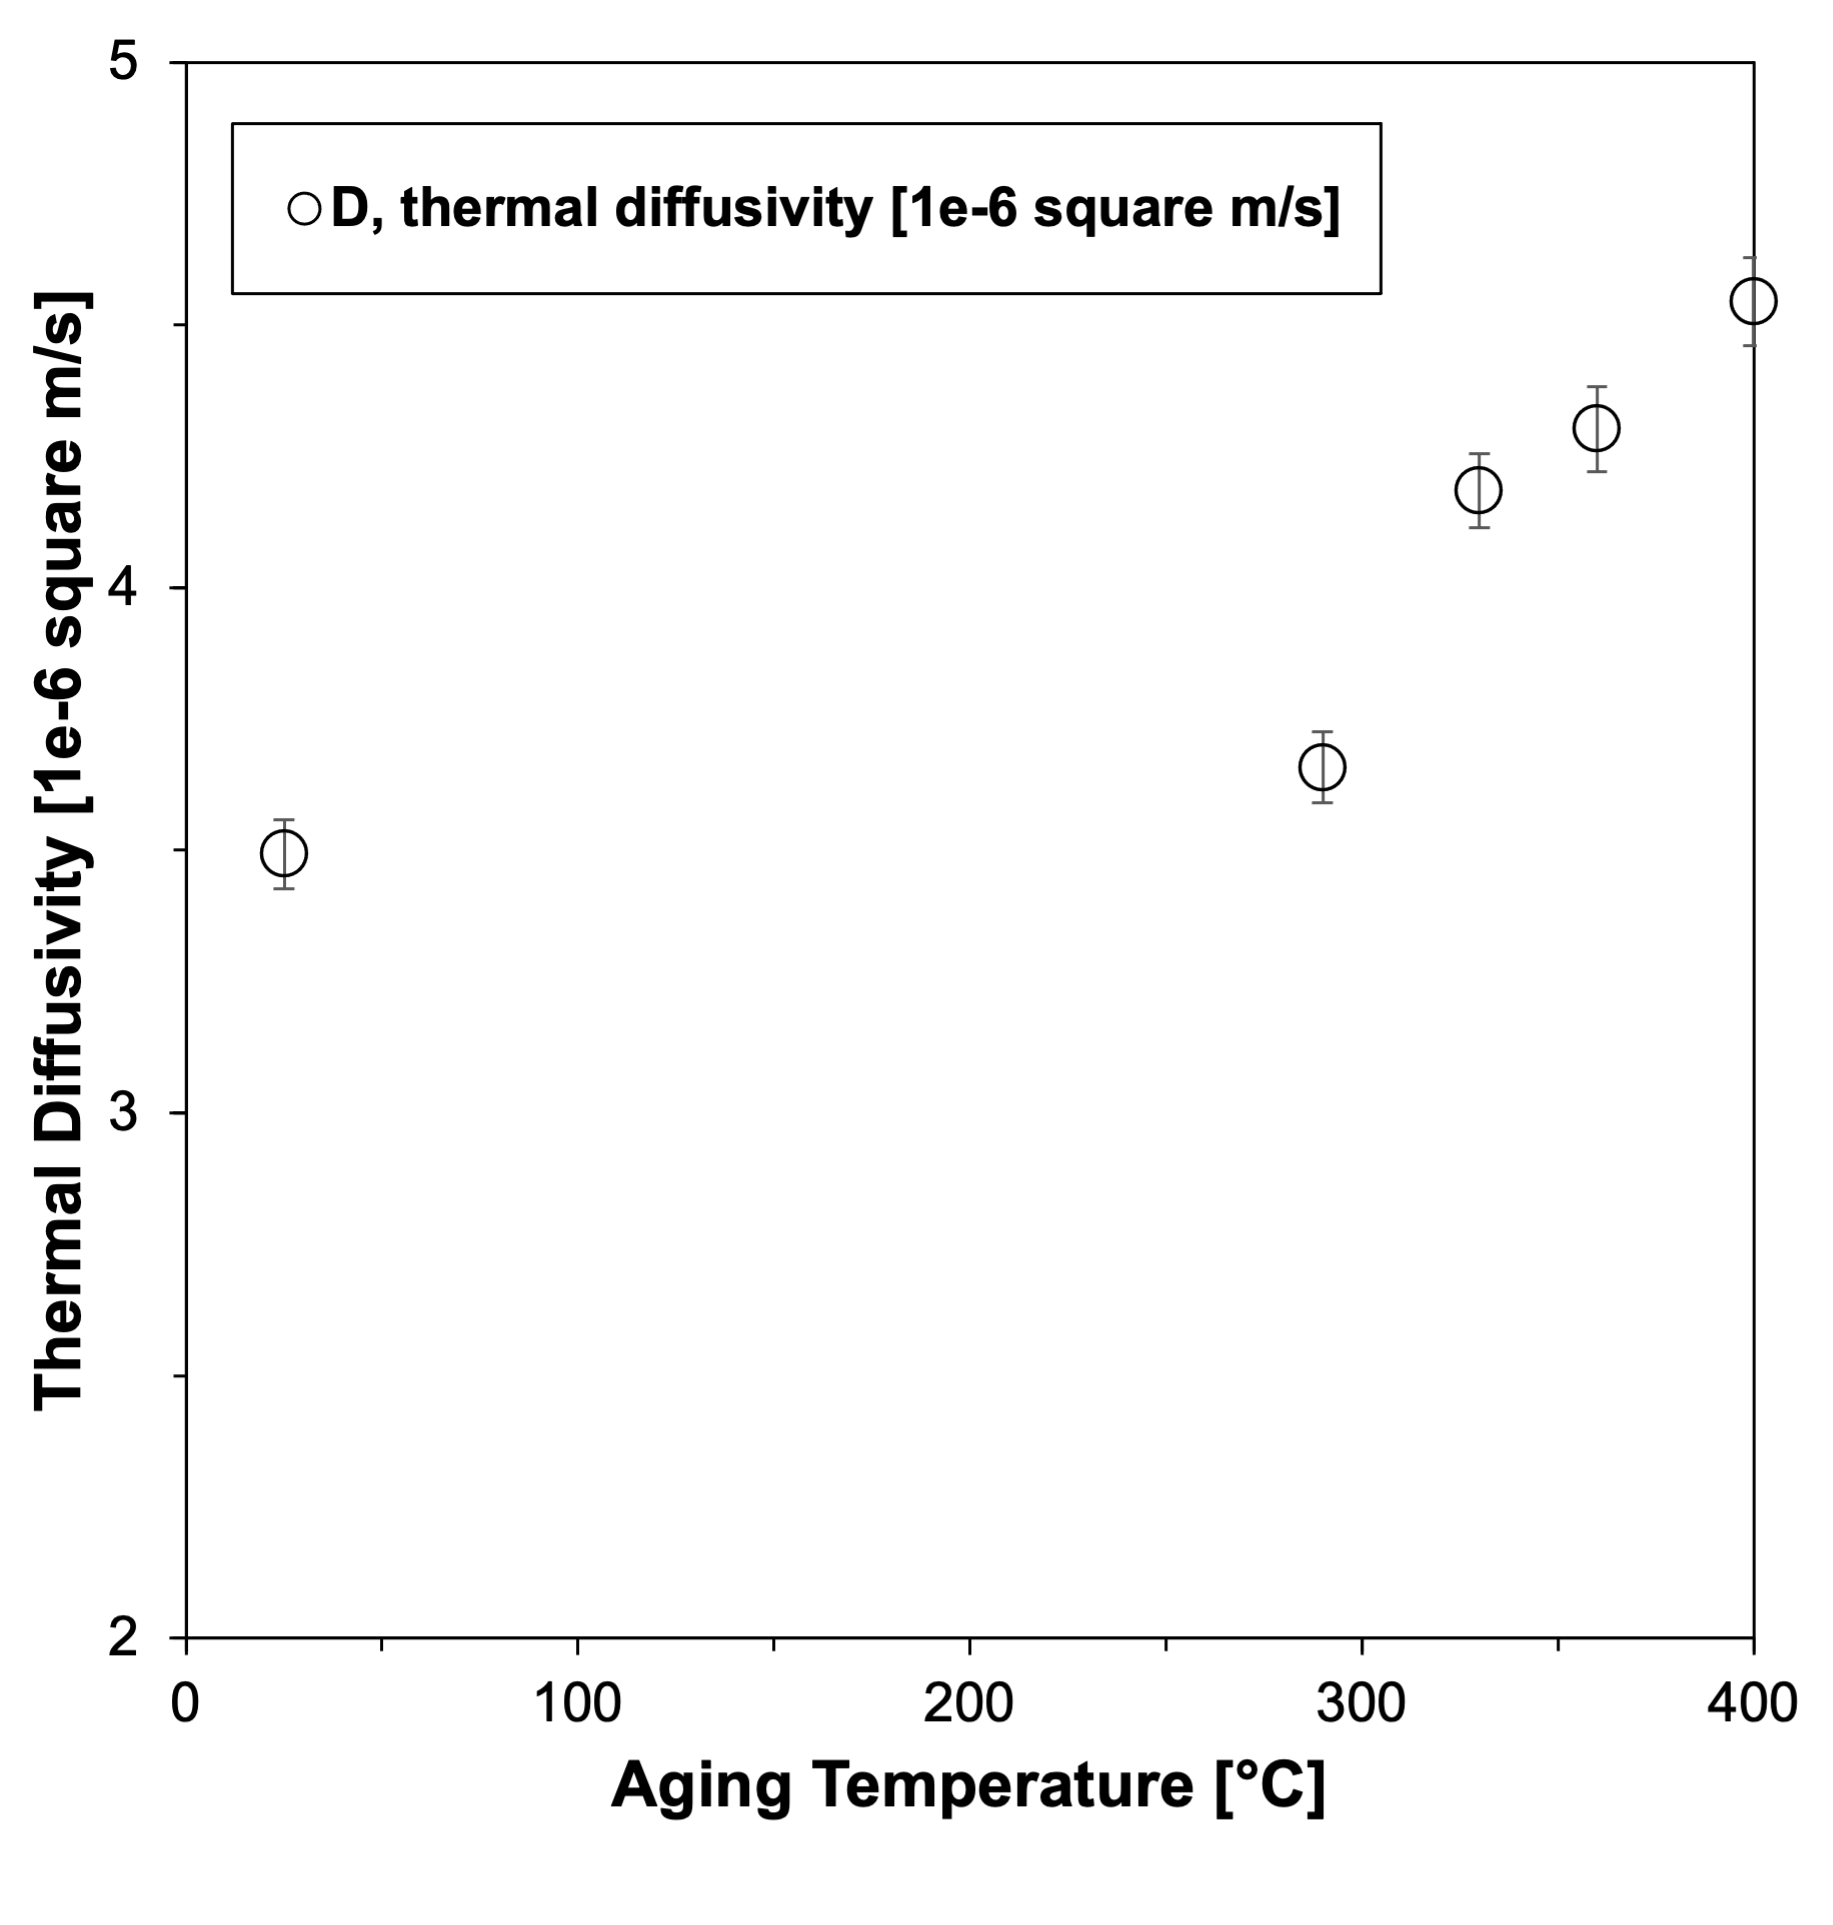
\includegraphics[width=\linewidth, right]{Parts/Figures/DvsT_CF8_30khrs_v2.png}         
\caption{$D^{exp}_{thermal}$, experimental thermal diffusivity [$\times 10^{-6} \frac{\text{m}^2}{\text{s}}$]}
         \label{fig5d}
     \end{subfigure}
          \hfill
     	\begin{subfigure}{0.3\textwidth}
         \centering
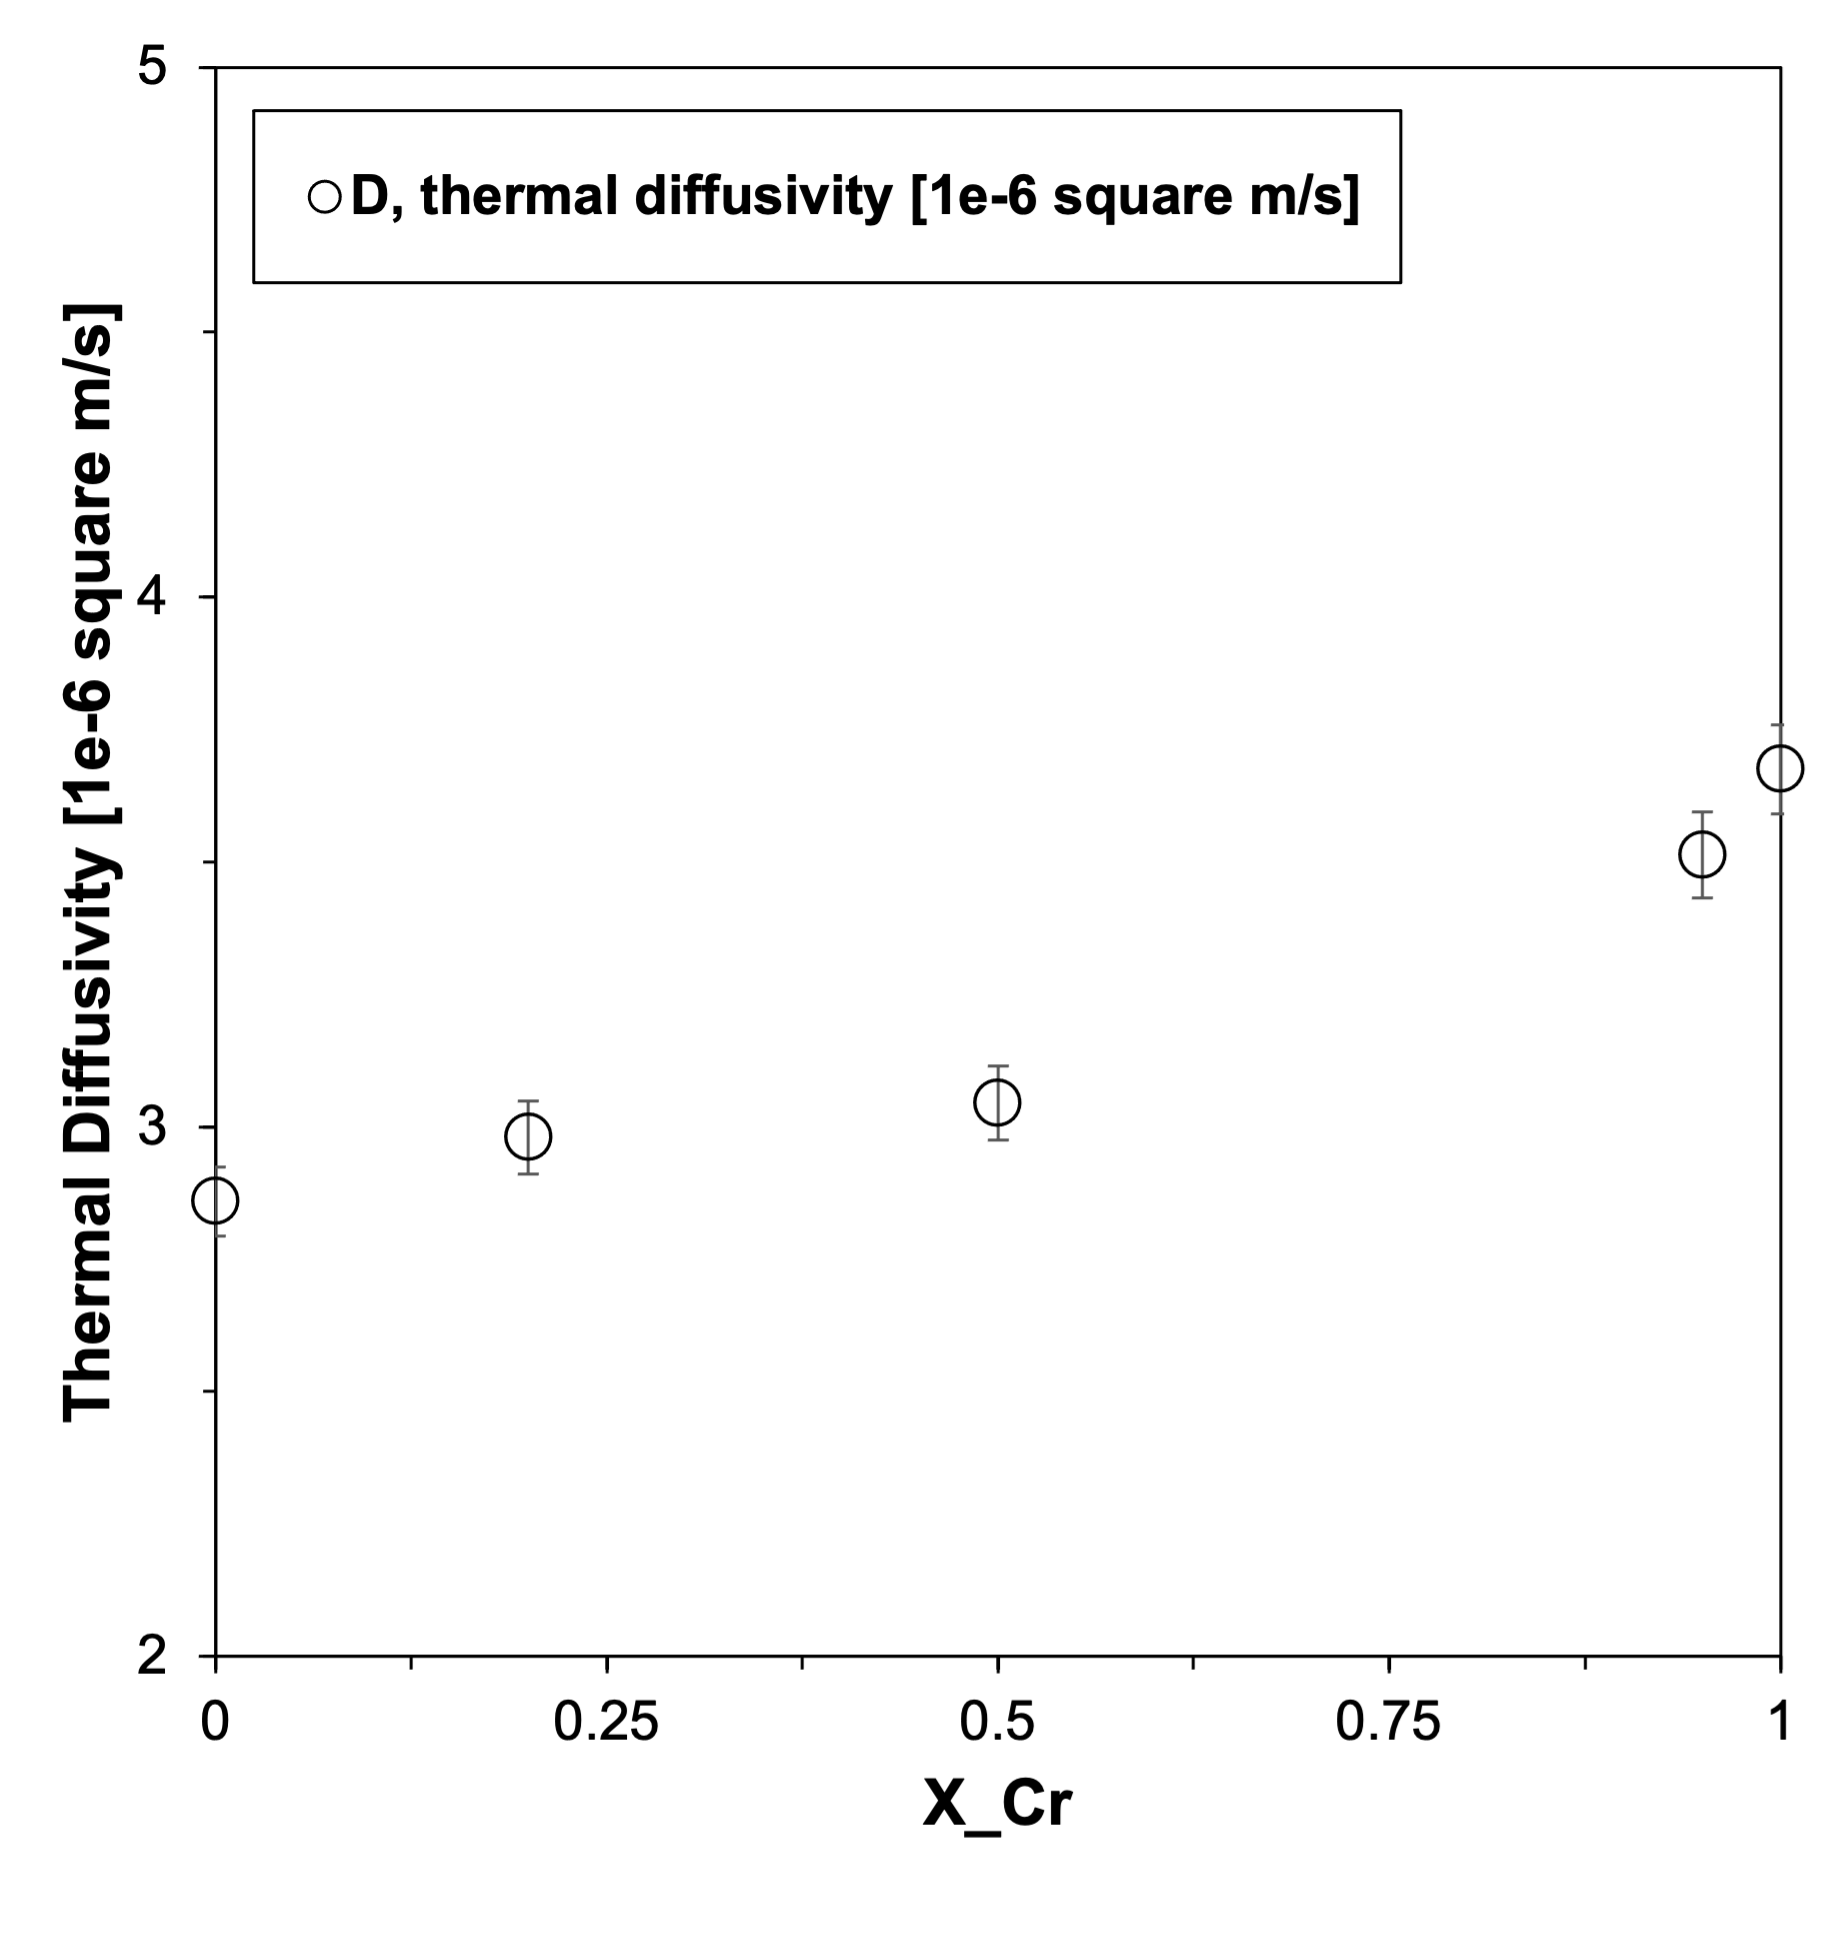
\includegraphics[width=\linewidth, left]{Parts/Figures/DvsX_v4.png}
         \caption{$D^{theoretical}_{thermal}$, theoretical thermal diffusivity [$\times 10^{-6} \frac{\text{m}^2}{\text{s}}$]}
         \label{fig5e}
     \end{subfigure}
          \hfill
     \begin{subfigure}{0.3\textwidth}
         \centering
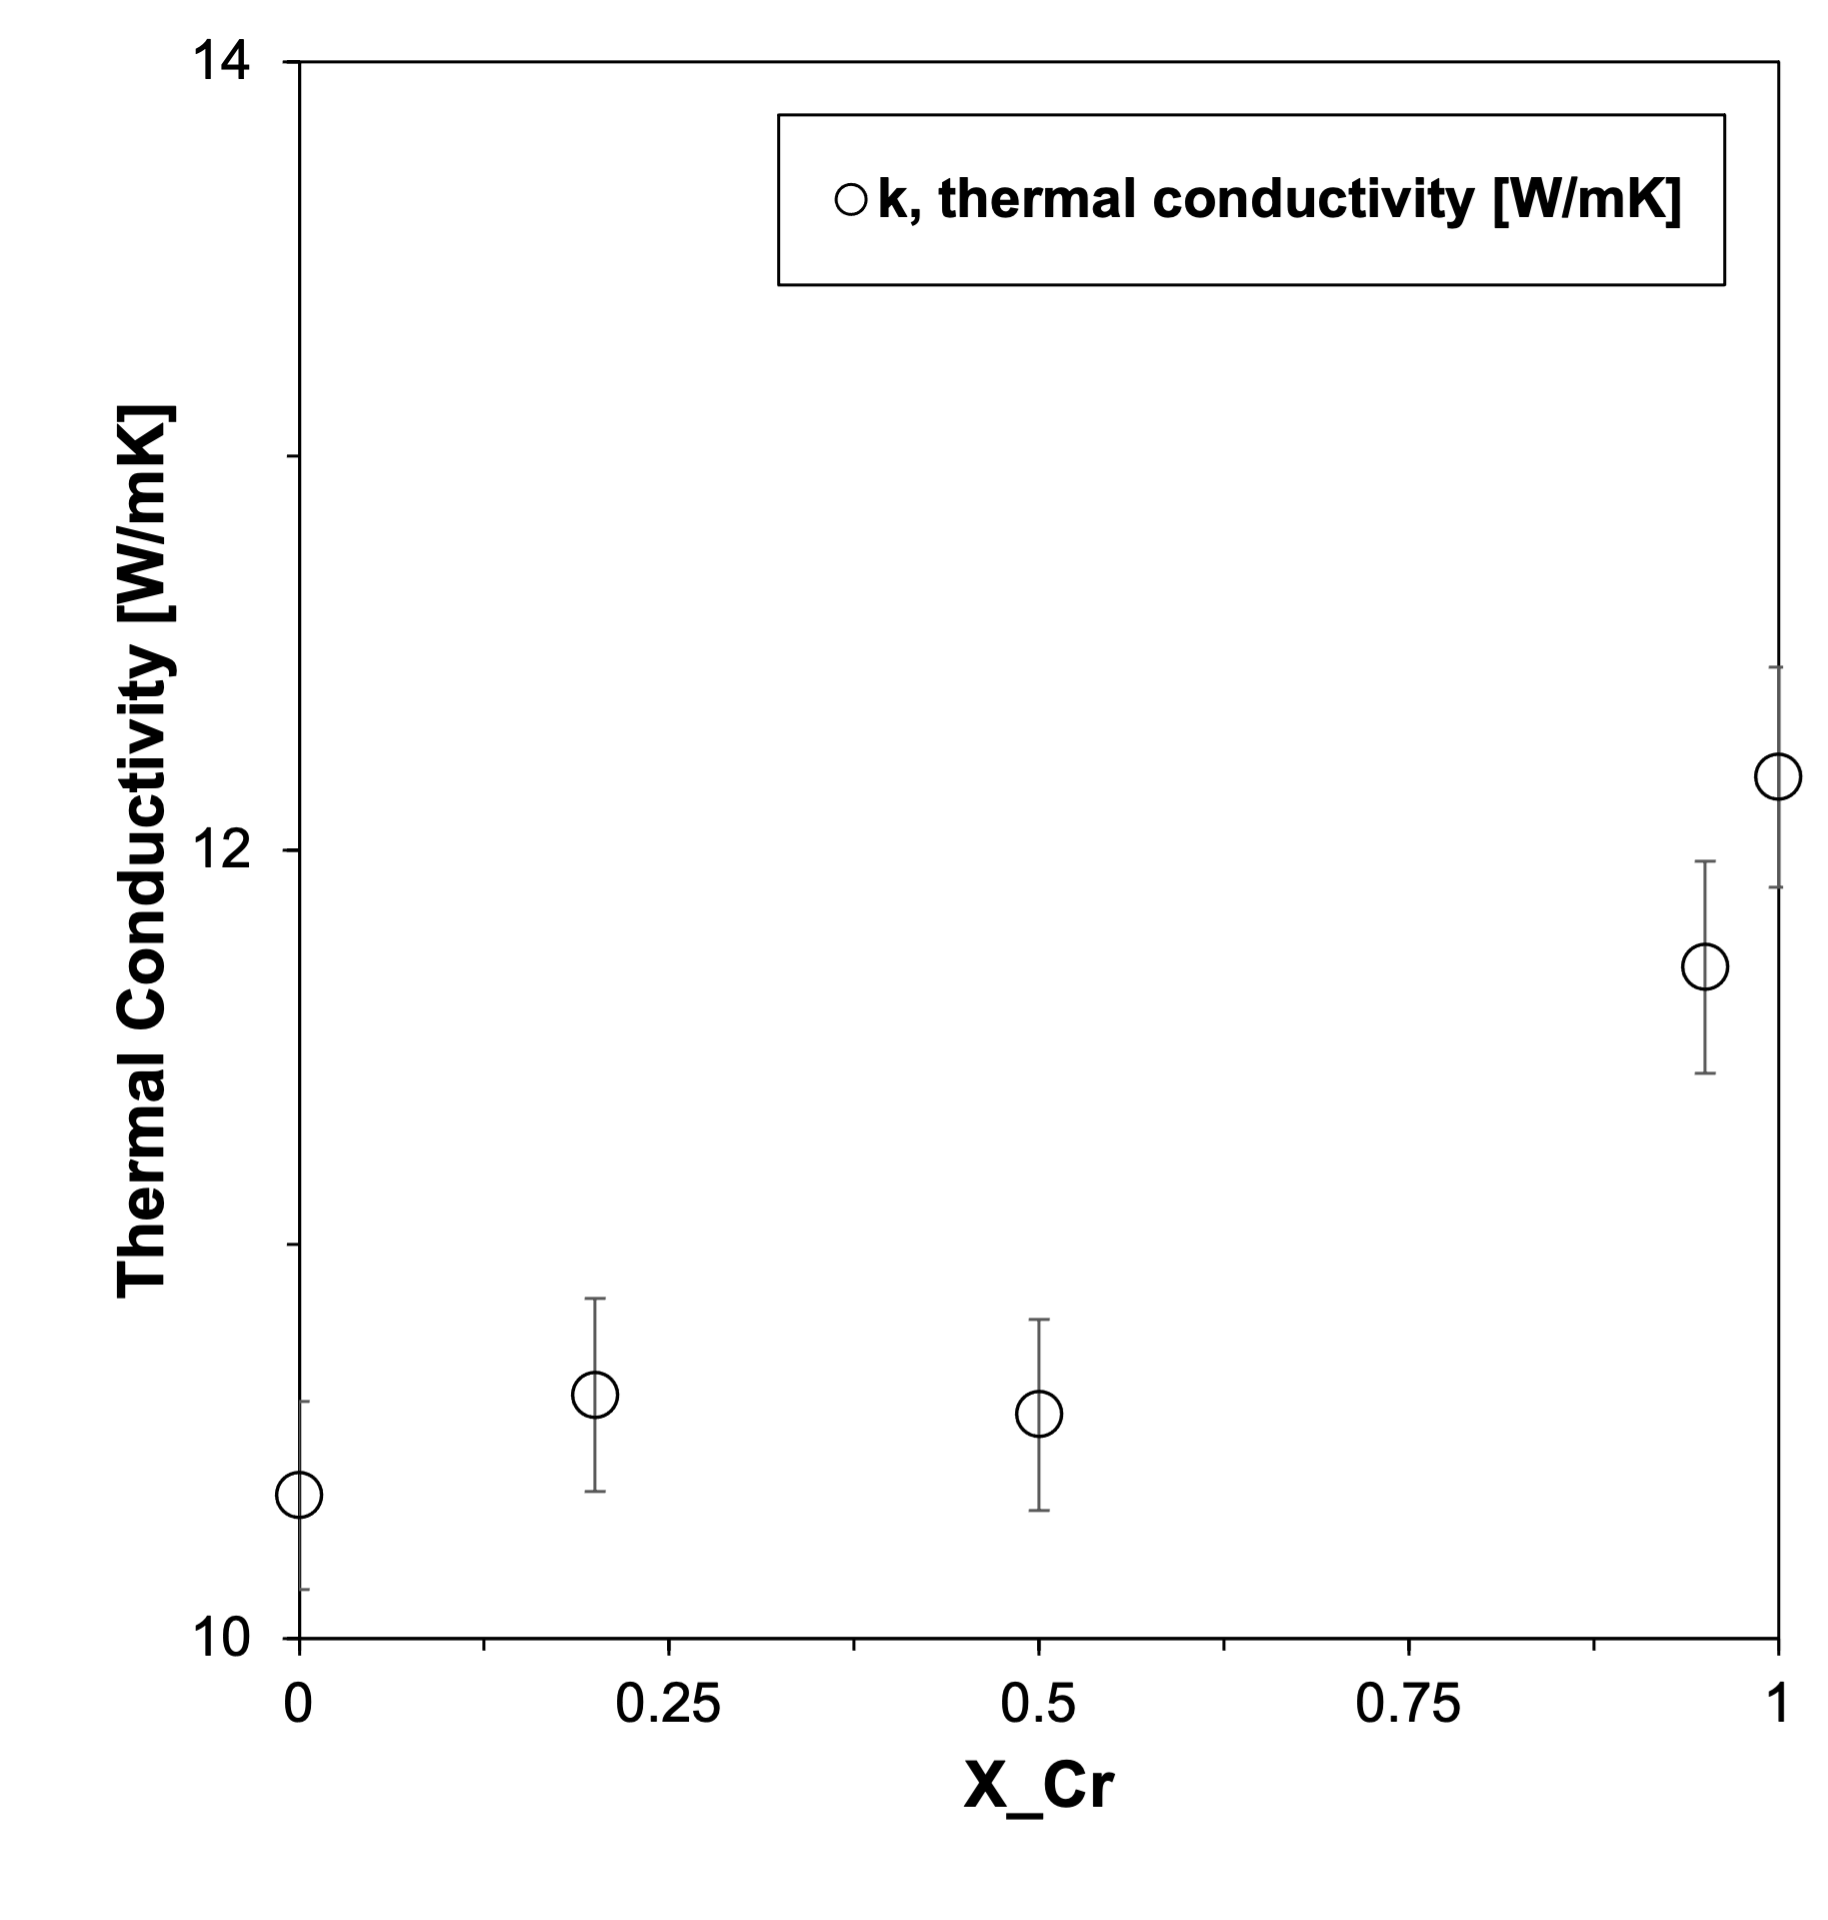
\includegraphics[width=\linewidth, right]{Parts/Figures/KvsX_v2.png}         \caption{$\kappa^{theoretical}_{thermal}$, thermal conductivity [$\frac{\text{W}}{\text{m}\cdot \text{K}}$]}
         \label{fig5f}
     \end{subfigure}
	\caption{(a) Elastic moduli as a function of aging temperature calculated from measured SAW frequencies for unaged and thermally aged 304 and 316-type stainless steel in [REF]. Elastic moduli for aged samples calculated from experimental SAW speeds are consistent with elastic moduli calculated from simplied density functional theory simulations of these alloys in Fig. \ref{fig3a}. As observed in [REF], the large error bounds in these values are due to the likelihood of a surface acoustic wave to probe both $\delta$-ferrite and $\gamma$-austenite, where $\delta$-ferrite grains are stiffened by spinodal decomposition and $\gamma$-austenite grains remain mechanically intact. However, the experimental and theoretical values consistently fall within the upper bounds on these calculations, consistent with density functional theory calculations in Fig. \ref{fig3a} combined with elastodynamic simulations in Fig. \ref{fig4a}. (b) ... (c) ... (d) experimental thermal diffusivity measured for 304-type stainless steel aged for 30,000 hours ... (e) ... (f) ...}
	\label{fig5}
\end{sidewaysfigure}